% \documentclass[a4paper,10pt]{report}
% \usepackage[utf8]{inputenc}
% \usepackage{amsmath}
% \usepackage{mathtools}
% \usepackage{graphicx}
% \usepackage{booktabs}
% \usepackage{caption}
% \usepackage{subcaption}
% \usepackage{float}
% \graphicspath{{images/}}
% 
% % Title Page
% \title{Navier Stokes Solver for two phase flow}
% \author{Palas Kumar farsoiya}

% 
% \begin{document}
% \maketitle
\chapter{Navier Stokes Solver for two phase flow}
% \begin{abstract}
% 
% \end{abstract}
\section{Governing Equations}
As we adopt continuum hypothesis, we then apply conservation principles to obtain governing equations for 
the fluid flow. These are conservation of mass, momentum and energy which are briefly described here. This derivation
is mostly adapted from \cite{Leal2007}.

\subsection{Mass conservation}
Consider a material volume element in Fig \ref{Fig:control_v}.  A material volume is one whose shape at time $t=0$, is arbitrary,
and has a fixed set of material points. And therefore, moves with the local continuum velocity of the fluid 
at every point.

\begin{wrapfigure}{r}{0.5\textwidth}
  \begin{center}
    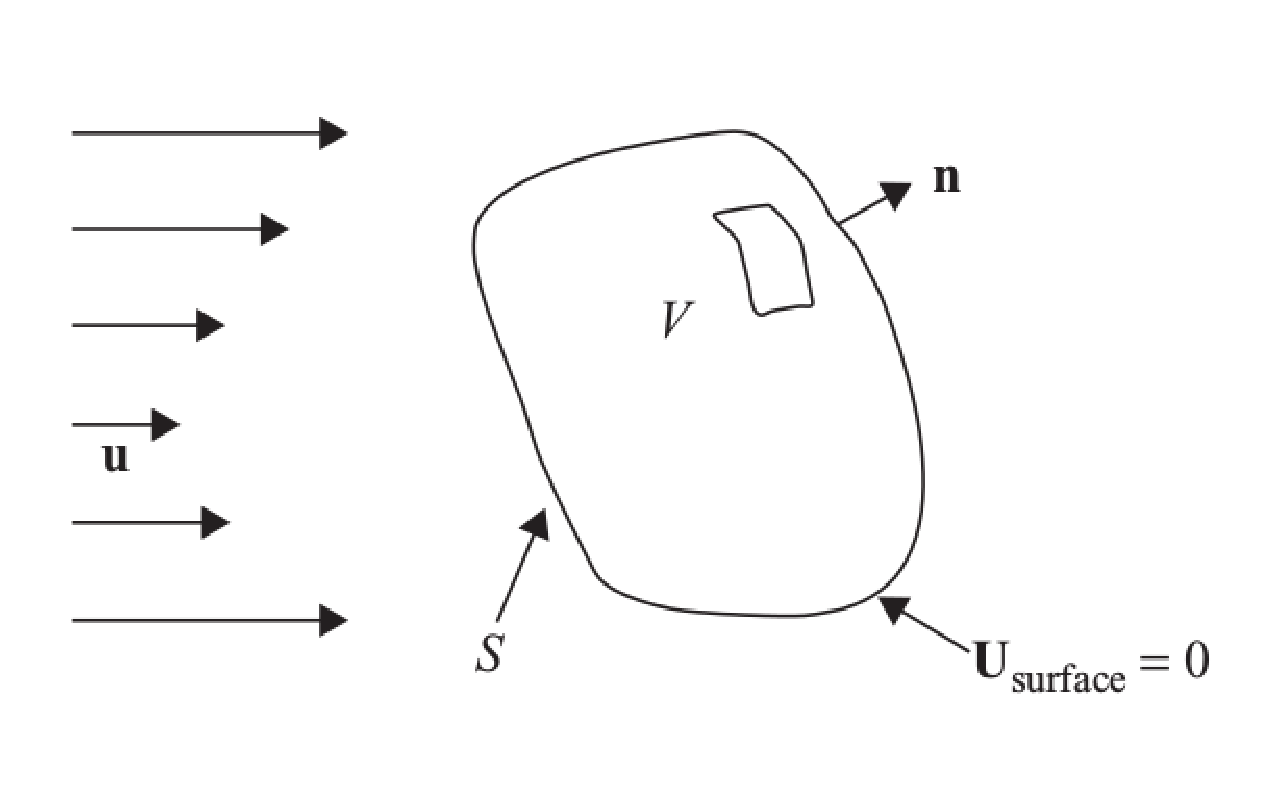
\includegraphics[width=0.48\textwidth]{control_v.eps}
  \end{center}
  \caption{An arbitrary control volume \cite{Leal2007}}
  \label{Fig:control_v}
\end{wrapfigure}

Conservation of mass states that mass is neither created nor destroyed. It implies that the mass inside the material volume is constant with respect
to time. Mathematically,
\begin{equation}
 \frac{D}{Dt}\left[\int_{V_m(t)}{\rho dV}\right] = 0 
 \label{Eq:1}
\end{equation}

where,
\begin{equation}
 \frac{DB}{Dt} = \frac{\partial B}{\partial t}+u.\nabla B
\end{equation}
Using the Reynolds transport theorem, which says

\begin{equation}
 \frac{D}{Dt}\left[\int_{V_m(t)}{}{B(x,t)}dV\right] = \int_{V_m(t)}{}{\left[\frac{\partial B}{\partial t} + \nabla . (Bu)\right] dV}
 \label{Eq:3}
\end{equation}

\ref{Eq:1}, can be written as, 
\begin{equation}
 \int_{V_m(t)}{}{\left[\frac{\partial \rho}{\partial t} + \nabla . (\rho u)\right] dV} = 0
\end{equation}

where the choice of $V_m(t)$ is arbitrary, hence the integrand itself must be zero.
\begin{equation}
 \frac{\partial \rho}{\partial t} + \nabla . (\rho u) = 0
 \label{Eq:5}
\end{equation}

For, incompressible fluids where density does not changes with time, \ref{Eq:5} reduces to,
\begin{equation}
 \nabla .u = 0
 \label{Eq:6}
\end{equation}

\subsection{Momentum Conservation}
Newton's second law states that,

\begin{equation}
 \textbf{Rate of change of linear momentum in an inertial frame} = \textbf{The sum of forces acting on the body}
\end{equation}

When we apply this to a material control volume, we obtain
\begin{equation}
 \frac{D}{Dt}\int_{V_m(t)} (\rho u) d V = \text{ sum of the forces acting on } V_m(t)
 \label{Eq:8}
\end{equation}

From a continuum perspective, the forces which act on the control volume can be of two types. Body force and surface force. The body force
which is common to most of the problems is gravitational force, which acts equally on all the volume elements. The surface forces are forces
are short range forces which acts on the surface of the control volume.

RHS of \ref{Eq:8}, can be expressed as sum of these two forces,
\begin{equation}
 \frac{D}{Dt}\int_{V_m(t)} (\rho u) d V = \int_{V_m(t)}{\rho g dV} + \int_{A_m(t)}{JdA}
 \label{Eq:9}
\end{equation}

where, g is acceleration due to gravity, $A_m(t)$ is the closed surface area of the control volume element and $J$ is the \textbf{stress vector}.
Using \ref{Eq:3}, we can write the RHS of \ref{Eq:9} as,

\begin{equation}
 \int_{V_m(t)}{}{\left[\frac{\partial (\rho u)}{\partial t} + \nabla . (\rho uu)\right] dV} =  \int_{V_m(t)}{\rho g dV} + \int_{A_m(t)}{JdA}
 \label{Eq:10}
\end{equation}

In the above equation stress vector $J$, can be found by linear vector operation on unit normal to the surface at any given point. The linear vector operator
is \textbf{T}, is called as stress tensor, which is a second order tensor. Thus, 

\begin{equation}
 J(n,x) = n . \textbf{T(x)} 
\end{equation}
Applying Gauss divergence theorem,
\begin{equation}
 \int_{A_m(t)}{n . \textbf{T}}dS  = \int_{V_m(t)}{\nabla . \textbf{T}} dV
\end{equation}
and substituting in \ref{Eq:10}, we get
\begin{equation}
 \int_{V_m(t)}{}{\left[\frac{\partial (\rho u)}{\partial t} + \nabla . (\rho uu)\right] dV} =  \int_{V_m(t)}{\rho g dV} + \int_{V_m(t)}{\nabla . \textbf{T}}
\end{equation}

After rearrangement, 
\begin{equation}
 \int_{V_m(t)}{\left[\frac{\partial (\rho u)}{\partial t} + \nabla . (\rho uu)  -  \rho g  - \nabla . \textbf{T}\right]dV} = 0
\end{equation}

Again, the $V_m(t)$, is an arbitrary control volume, and the integrand must be then zero. Thus we obtain,

\begin{equation}
 \frac{\partial (\rho u)}{\partial t} + \nabla . (\rho uu)  =  \rho g  + \nabla . \textbf{T} 
 \label{Eq:15}
\end{equation}

The stress tensor \textbf{T} can be expressed in terms of isotropic and non-isotropic parts,

\begin{equation}
 \textbf{T} = -p\textbf{I}+\textbf{$\tau$ }
\end{equation}
Substitute this form in \ref{Eq:15}, we get

\begin{equation}
 \frac{\partial (\rho u)}{\partial t} + \nabla . (\rho uu)  = \nabla .( -p\textbf{I}+\tau) + \rho g  
 \label{Eq:17}
\end{equation}
The constitutive equation for a Newtonian fluid is,
\begin{equation}
 \textbf{$\tau$} = 2\mu \textbf{D}
 \label{Eq:18}
\end{equation}
where, \textbf{$D$} is the rate of strain tensor, the symmetric part of $\nabla u$. Now,
\begin{equation}
 \text{$\tau$} = \mu (\nabla u + (\nabla u)^T)
 \label{Eq:19}
\end{equation}

Substituting this in \ref{Eq:17}, we get
\begin{equation}
 \frac{\partial (\rho u)}{\partial t} + \nabla . (\rho uu)  =  -\nabla p+ \nabla .(\mu (\nabla u + (\nabla u)^T)) + \rho g  
 \label{Eq:20}
\end{equation}
Subtracting \ref{Eq:5} from \ref{Eq:20}, we get
\begin{equation}
 \frac{\partial u}{\partial t} + (u.\nabla)u  =  -\frac{\nabla p}{\rho}+ \frac{1}{\rho}\nabla .(\mu (\nabla u + (\nabla u)^T)) +  g   
 \label{Eq:21}
\end{equation}
Rewriting \ref{Eq:21}, in conservative form, using mass conservation
\begin{equation}
 \frac{\partial u}{\partial t} + \nabla .(uu)  =  -\frac{\nabla p}{\rho}+ \frac{1}{\rho}\nabla .(\mu (\nabla u + (\nabla u)^T)) +  g  
 \label{Eq:22}
\end{equation}

\subsection{Non-Dimensionalisation of governing equations}
For non-dimensionalisation we chose scale as characteristic length  L, characteristic velocity U, characteristic time $\frac{L}{U}$, characteristic pressure $\rho_L U^2$,
characteristic density $\rho_L$ and characteristic viscosity $\mu_L$.
Substitute $u = U\tilde u $, $x = L\tilde x $, $y = L\tilde y $, $t = \frac{L}{U}\tilde t $, $p = \rho_L U^2\tilde p $, $\rho = \rho_L \tilde\rho $, $\mu = \mu_L \tilde\mu $
in \ref{Eq:22}, where quantities with tilde are non-dimensional.

\begin{equation}
 \frac{U^2}{L}\left[\frac{\partial \tilde u}{\partial \tilde t} + \tilde\nabla .(\tilde u \tilde u)\right]  = -\frac{\rho_L}{\rho_L \tilde\rho}\frac{U^2}{L}\tilde\nabla \tilde p
 + \frac{U^2}{L^2\rho_L \tilde\rho}\tilde \nabla .(\mu_L \tilde\mu (\tilde\nabla \tilde u + (\tilde\nabla \tilde u)^T)) +  g 
 \label{Eq:23}
\end{equation}

Rearranging \ref{Eq:23},

\begin{equation}
 \left[\frac{\partial \tilde u}{\partial \tilde t} + \tilde\nabla .(\tilde u \tilde u)\right]  = -\frac{1}{\tilde\rho}\tilde\nabla \tilde p
 + \frac{\mu_L}{L\rho_L U}\frac{1}{\tilde\rho}\tilde \nabla .(\tilde\mu (\tilde\nabla \tilde u + (\tilde\nabla \tilde u)^T)) +  \frac{gL}{U^2} 
 \label{Eq:24}
\end{equation}

Now, dropping tilde from the quantities,
\begin{equation}
 \frac{\partial  u}{\partial  t} + \nabla .( u  u)  = -\frac{1}{\tilde\rho}\nabla  p
 + \frac{1}{Re_L}\frac{1}{\tilde\rho} \nabla .(\tilde\mu (\nabla  u + (\nabla  u)^T)) +  \frac{1}{Fr^2} 
 \label{Eq:25}
\end{equation}

where, $Re_L = \frac{L\rho_L U}{\mu_L}$, $We_L = \frac{L \rho_L U^2}{\sigma_{LG}}$ and $Fr = \frac{U}{\sqrt{gL}}$. 

\ref{Eq:25} is the non-dimensional form for incompressible multiphase newtonian flow.

\subsection{Integral form of governing equation}
As the conservation equations are valid for a differential element, we can also integrate them over a control volume. This is the final step before the finite volume discretisation
approach.\ref{Eq:25} can be integrated on a control volume, V 

\begin{equation}
\int_V\left[ \frac{\partial  u}{\partial  t} + \nabla .( u  u)\right]dV  = \int_V\left[-\frac{1}{\tilde\rho}\nabla  p
 + \frac{1}{Re_L}\frac{1}{\tilde\rho} \nabla .(\tilde\mu (\nabla  u + (\nabla  u)^T)) +  \frac{1}{Fr^2}\right]dV 
 \label{Eq:26}
\end{equation}

\begin{equation}
\int_V \frac{\partial  u}{\partial  t}dV +\int_V \nabla .( u  u)dV  = -\int_V\frac{1}{\tilde\rho}\nabla  p dV
 + \frac{1}{Re_L}\frac{1}{\tilde\rho} \int_V\nabla .(\tilde\mu (\nabla  u + (\nabla  u)^T))dV +  \frac{1}{Fr^2}\int_V dV \nonumber \\
 \label{Eq:27}
\end{equation}
Applying Gauss divergence theorem on advection and diffusion intergrals, we get
\begin{equation}
\int_V \frac{\partial  u}{\partial  t}dV +\int_S u(u.n)dS  = -\int_V\frac{1}{\tilde\rho}\nabla  p dV
 + \frac{1}{Re_L}\frac{1}{\tilde\rho} \int_S (\tilde\mu (\nabla  u + (\nabla  u)^T).n)dS +  \frac{1}{Fr^2}\int_VdV \nonumber \\
 \label{Eq:28}
\end{equation}

Now, we can average the individual quantities over the control volume, V and Equation \ref{Eq:29} is used for discretisation in our code.
\begin{eqnarray}
\frac{1}{V}\int_V \frac{\partial  u}{\partial  t}dV +\frac{1}{V}\int_S u(u.n)dS  = -\frac{1}{V}\int_V\frac{1}{\tilde\rho}\nabla  p dV \nonumber
 + \frac{1}{Re_L}\frac{1}{\tilde\rho} \frac{1}{V}\int_S (\tilde\mu (\nabla  u + (\nabla  u)^T).n)dS \nonumber \\
 +  \frac{1}{Fr^2}\frac{1}{V}\int_VdV \nonumber \\
 \label{Eq:29}
\end{eqnarray}

\section{Discretisation of governing equations}
\subsection{Grid}
 \setlength\intextsep{0pt}
\begin{wrapfigure}{r}{0.4\textwidth}
  \begin{center}
    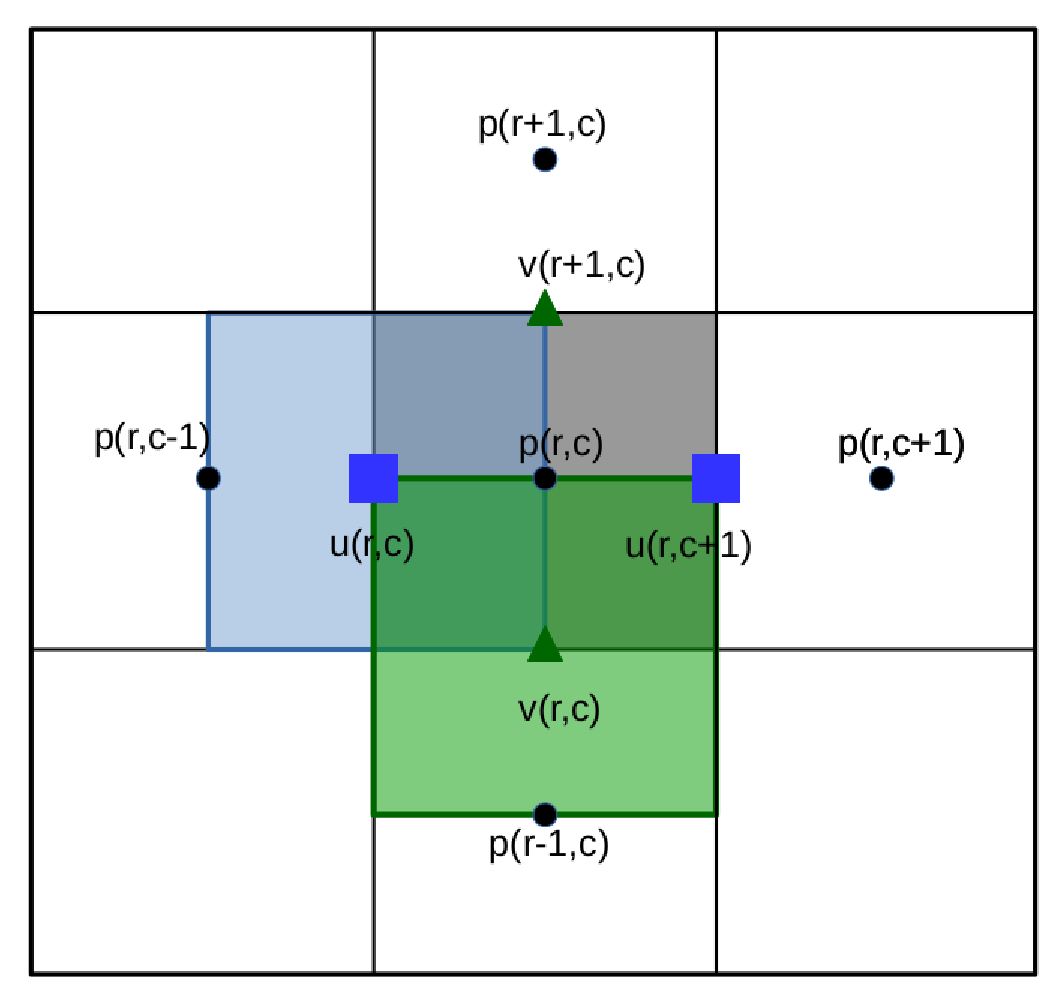
\includegraphics[width=0.4\textwidth]{grid_st.eps}
  \end{center}
  \caption{Staggered grid for x-velocity(Blue),y-velocity(Green) and pressure(Gray)}
  \label{Fig:grid_st}
\end{wrapfigure}
Before discretisation, we first specify our domain, grid shape and approach. The grid is rectangular and uniform grid spacing has been used for both x and y directions.
Figure \ref{Fig:grid_st} and \ref{Fig:grid} shows the grid and location of pressure and velocity nodes.
We can see the nodes of pressure and velocities are not colocated because decoupling of pressure and velocity may occur since the discretised form of equation of continuity 
on colocated grids can lead to checkerboard patterns in the solution(\cite{Anderson1995}). Staggered grid approach is used to avoid pressure-velocity decoupling. 
There are three different grids for x-velocity (u),y- velocity(v) and pressure (p).  
The momentum equation are discretised using finite volume approach using the conservative form of equations. This would first order in time and a predictor-corrector approach to 
compute velocity field in the domain.
 \begin{figure}
 \centering
  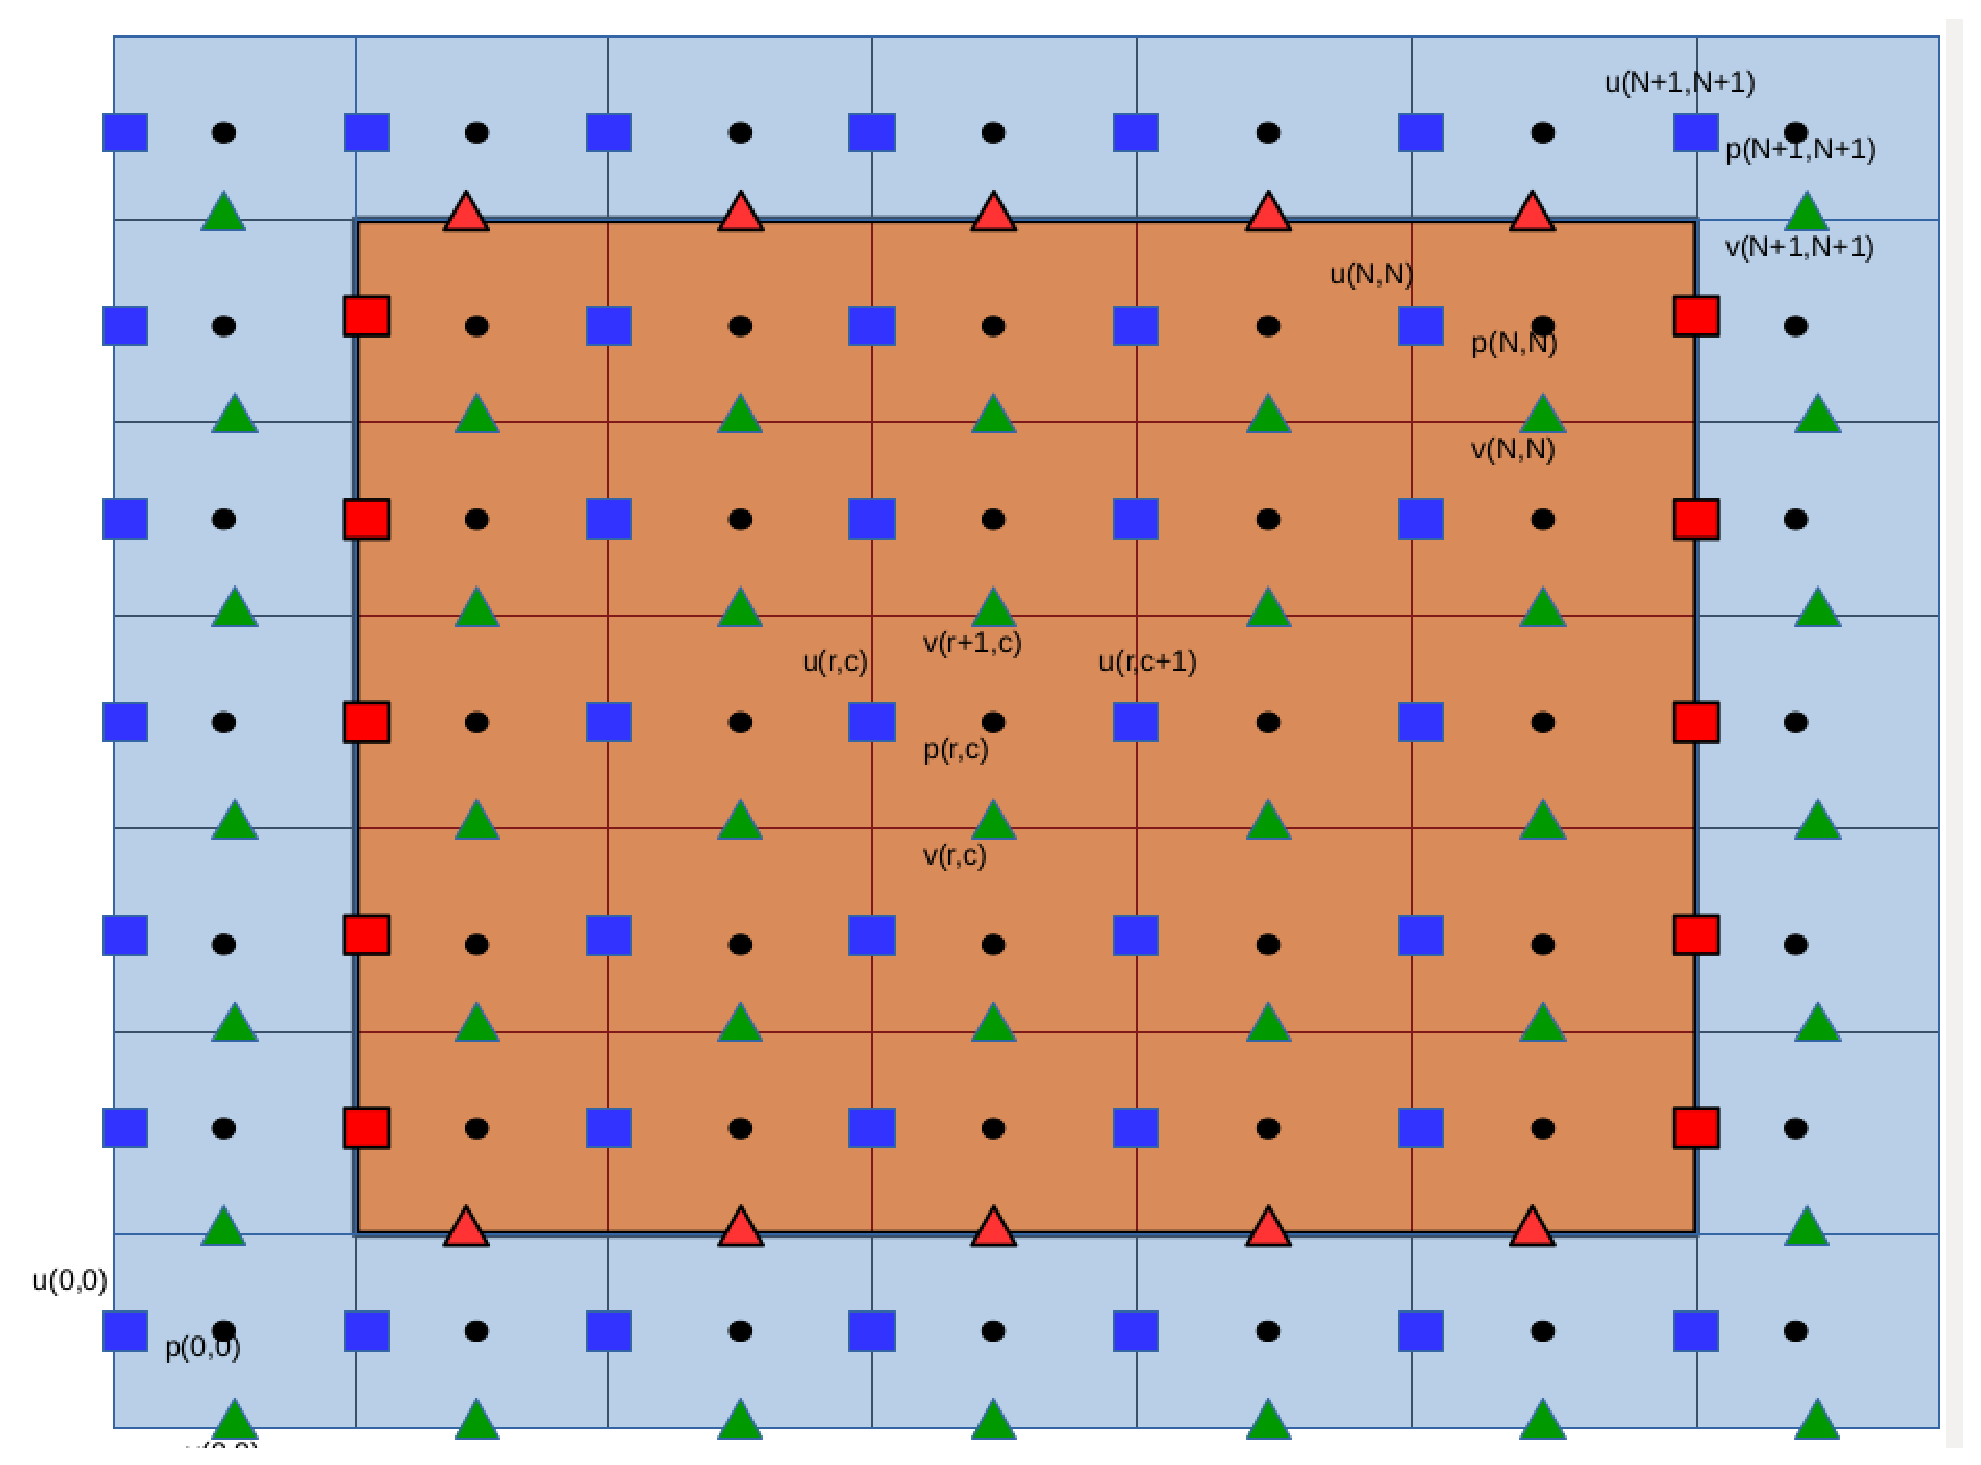
\includegraphics[scale=0.3]{pressure_calc.eps}
  \caption{Location of nodes, blue square:x-velocity, red square:boundary x-velocity, green triangle:y-velocity, red triangle:boundary y-velocity,black dot:pressure}
  \label{Fig:grid}
 \end{figure}


\subsection{Integration in time}
The first step is  to compute projected velocity, ignoring the pressure terms, 
\begin{equation}
 \frac{u^*-u^n}{\Delta t} =  -A^n + D^n + B^n
\end{equation}
where $u^n$ is the velocity at previous time step and $u^*$ is the projected velocity without taking pressure into consideration, 
where $A = \frac{1}{V}\int_S u(u.\hat{n})dS$ ,\\ \\ $D =\frac{1}{V}\frac{1}{Re_L}\frac{1}{\tilde\rho} \frac{1}{V}\int_S (\tilde\mu (\nabla  u + (\nabla  u)^T).\hat{n})dS $ and \\ \\
$B = \frac{1}{Fr^2}\frac{1}{V}\int_VdV  $
And then adding the pressure component in the projected velocity,

\begin{equation}
 \frac{u^{n+1}-u^*}{\Delta t} = -\frac{1}{V}\int_V\frac{1}{\rho}\nabla  p^{n+1} dV
\end{equation}

Rearranging,
\begin{equation}
 u^{n+1} = u^*-\frac{\Delta t}{V}\int_V\frac{1}{\rho}\nabla  p^{n+1} dV
\end{equation}

\subsection{Discretisation of advection terms}
To evaluate the advection terms, integrate it over the surface of the control volume. It is actually the sum of in and out fluxes through the faces of control volume. 
Here an approximation is made by assuming a uniform velocity on the faces of control volume and the fluxes are thus calculated by the value at the center of the boundary. 
Weighted Essentially Non-Oscillatory(WENO) [\cite{liu1994weighted}, \cite{jiang1995efficient}] scheme has been used to approximate the values of velocities at the face centers.
\begin{figure}
 \centering
 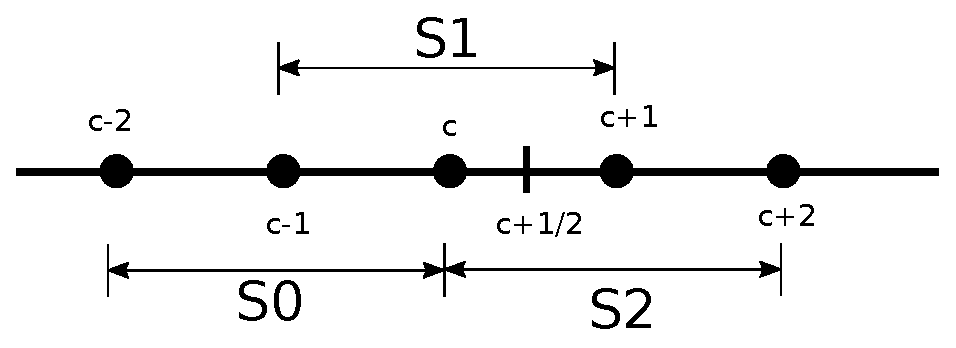
\includegraphics{wen_stencil.eps}
 \caption{Three sub stencils for reconstruction of $u_{i+1/_2}$}
\end{figure}

\begin{eqnarray*}
u^{(0)}_{c+1/_2} &=& \frac{1}{3}u_{c-2} - \frac{7}{6}u_{c-1} + \frac{11}{6} u_{c} \\
u^{(1)}_{c+1/_2} &=& -\frac{1}{6}u_{c-1} + \frac{5}{6}u_{c} + \frac{1}{3}u_{c+1} \\
u^{(2)}_{c+1/_2} &=& \frac{1}{3}u_{c} + \frac{5}{6}u_{c+1} − \frac{1}{6}u_{c+2} \\
\end{eqnarray*}

Once we get $u^{k}_{c+1/_2}$ from the three sub-stencils, we can get,
\begin{equation}
 u_{c+1/_2} = \sum_{k=0}^2 \omega_k u^{(k)}_{c+1/_2} %+ \omega_1 u^{(1)}_{c+1/_2} + \omega_2 u^{(2)}_{c+1/_2}
\end{equation}
where $\omega_k$ is given by,
\begin{eqnarray*}
 \omega_k = \frac{\tilde\omega_k}{\sum_{k=0}^2 \tilde\omega_k}, \qquad
 \tilde\omega_k = \frac{\gamma_k}{(\epsilon+\beta_k)^2} \\
 \gamma_0 = \frac{1}{10}, \quad \gamma_1 = \frac{3}{5}, \quad\text{and}\quad \gamma_2 = \frac{3}{10} \\
  \epsilon = 10^{-6}
\end{eqnarray*}
And, smoothness indicator $\beta_k$ is given by,
\begin{eqnarray*}
\beta_0 &=& \frac{13}{12}(u_{c-2} - 2u_{c-1} + u_c)^2 + \frac{1}{4}(u_{c-2}-4u_{c-1}+3u_c)^2\\
\beta_1 &=& \frac{13}{12}(u_{c-1} - 2u_{c} + u_{c+1})^2 + \frac{1}{4}(u_{c-1}-u_{c+1})^2\\
 \beta_2 &=& \frac{13}{12}(u_{c} - 2u_{c+1} + u_{c+2})^2 + \frac{1}{4}(3u_{c}-4u_{c+1}+u_{c+2})^2\\
\end{eqnarray*}

\begin{eqnarray}
 (A_x)_{net} &=& \frac{1}{V}\int_S u(u.n)dS \\
	 &=& \frac{1}{\Delta x \Delta y}\left[\int_{right} u(u.n)ds - \int_{left} u(u.n)ds + \int_{top} u(u.n)ds - \int_{bottom} u(u.n)ds\right] \nonumber \\
 \end{eqnarray}
% \begin{eqnarray*}
% \int_{right} u(u.n)ds &=& \left[\left(\frac{u_{r,c+1}+u_{r,c}}{2}\right)^2\right]\Delta y \\
% \int_{left} u(u.n)ds &=& \left[\left(\frac{u_{r,c}+u_{r,c-1}}{2}\right)^2\right]\Delta y \\
% \int_{top} u(u.n)ds &=& \left[\left(\frac{v_{r+1,c}+v_{r+1,c-1}}{2}\right)\left(\frac{u_{r+1,c}+u_{r,c}}{2}\right)\right]\Delta x \\
% \int_{top} u(u.n)ds &=& \left[\left(\frac{v_{r,c}+v_{r,c-1}}{2}\right)\left(\frac{u_{r,c}+u_{r-1,c}}{2}\right)\right]\Delta x \\
% \end{eqnarray*}
% Now, $(A_x)_{net}$ is now given by,
%  \begin{eqnarray*}
%  (A_x)_{net} =  \frac{1}{\Delta x}\left[\left(\frac{u_{r,c+1}+u_{r,c}}{2}\right)^2-\left(\frac{u_{r,c}+u_{r,c-1}}{2}\right)^2\right] \\
%  + \frac{1}{\Delta y}\left[\left(\frac{v_{r+1,c}+v_{r+1,c-1}}{2}\right)\left(\frac{u_{r+1,c}+u_{r,c}}{2}\right) 
%  -\left(\frac{v_{r,c}+v_{r,c-1}}{2}\right)\left(\frac{u_{r,c}+u_{r-1,c}}{2}\right)\right]
%  \end{eqnarray*}
% Similarly, $(A_y)_{net}$ is,
%   \begin{eqnarray*}
%  (A_y)_{net} =   \frac{1}{\Delta x}\left[\left(\frac{v_{r,c+1}+v_{r,c}}{2}\right)\left(\frac{u_{r,c+1}+u_{r-1,c+1}}{2}\right) 
%  -\left(\frac{v_{r,c}+v_{r,c-1}}{2}\right)\left(\frac{u_{r,c}+u_{r-1,c}}{2}\right)\right] \\
%  +\frac{1}{\Delta y}\left[\left(\frac{v_{r,c+1}+v_{r,c}}{2}\right)^2-\left(\frac{v_{r,c}+v_{r,c-1}}{2}\right)^2\right]
%  \end{eqnarray*}
 
 \subsection{Diffusion terms}
 Before looking at the discretised form of diffusion terms, we shall derive the components for x and y directions.
 
\subsubsection{Components of Diffusion term}
Gradient of velocity for 2D flow, 
\begin{equation*}
 \nabla u =  \begin{bmatrix} \frac{\partial u}{\partial x} & \frac{\partial u}{\partial y} \\ \frac{\partial v}{\partial x} & \frac{\partial v}{\partial y}  \end{bmatrix}
\end{equation*}

\begin{equation*}
 \nabla u + (\nabla u)^T=  \begin{bmatrix} \frac{\partial u}{\partial x} & \frac{\partial u}{\partial y} \\ \frac{\partial v}{\partial x} & \frac{\partial v}{\partial y}  \end{bmatrix}
 + \begin{bmatrix} \frac{\partial u}{\partial x} & \frac{\partial v}{\partial x} \\ \frac{\partial u}{\partial y} & \frac{\partial v}{\partial y}  \end{bmatrix}
\end{equation*}
\begin{equation*}
 \nabla u + (\nabla u)^T=  \begin{bmatrix} 2\frac{\partial u}{\partial x} & \left(\frac{\partial u}{\partial y}+\frac{\partial v}{\partial x}\right) \\ 
 \left(\frac{\partial u}{\partial y}+\frac{\partial v}{\partial x}\right) & 2\frac{\partial v}{\partial y}  \end{bmatrix}
\end{equation*}
\begin{equation*}
 (\tilde\mu (\nabla  u + (\nabla  u)^T)) = \begin{bmatrix} 2\tilde\mu\frac{\partial u}{\partial x} & \tilde\mu\left(\frac{\partial u}{\partial y}+\frac{\partial v}{\partial x}\right) \\ 
 \tilde\mu\left(\frac{\partial u}{\partial y}+\frac{\partial v}{\partial x}\right) & 2\tilde\mu\frac{\partial v}{\partial y}  \end{bmatrix}
\end{equation*}

% Now, taking divergence of the above tensor,
% 
% \begin{equation}
%  \nabla .(\tilde\mu (\nabla  u + (\nabla  u)^T)) = \begin{bmatrix}\frac{\partial}{\partial x} & \frac{\partial}{\partial y} \end {bmatrix}
%  \begin{bmatrix} 2\tilde\mu\frac{\partial u}{\partial x} & \tilde\mu\left(\frac{\partial u}{\partial y}+\frac{\partial v}{\partial x}\right) \\ 
%  \tilde\mu\left(\frac{\partial u}{\partial y}+\frac{\partial v}{\partial x}\right) & 2\tilde\mu\frac{\partial v}{\partial y}  \end{bmatrix}
% \end{equation}
% we get,
% \begin{equation}
%  \nabla .(\tilde\mu (\nabla  u + (\nabla  u)^T)) \\
%  \\
%  = \begin{bmatrix}\frac{\partial}{\partial x}\left(2\tilde\mu\frac{\partial u}{\partial x}\right) 
%  + \frac{\partial}{\partial y}\left(\tilde\mu\left(\frac{\partial u}{\partial y}+\frac{\partial v}{\partial x}\right)\right) \\
%  \frac{\partial}{\partial x}\left(\tilde\mu\left(\frac{\partial u}{\partial y}+\frac{\partial v}{\partial x}\right)\right) 
%  + \frac{\partial}{\partial y}\left(2\tilde\mu\frac{\partial v}{\partial y}\right)
%  \end {bmatrix}
% \end{equation}
\begin{eqnarray*}
 (\tilde\mu (\nabla  u + (\nabla  u)^T))_x = \begin{bmatrix} 2\tilde\mu\frac{\partial u}{\partial x} & \tilde\mu\left(\frac{\partial u}{\partial y}+\frac{\partial v}{\partial x}\right) \\ 
 \tilde\mu\left(\frac{\partial u}{\partial y}+\frac{\partial v}{\partial x}\right) & 2\tilde\mu\frac{\partial v}{\partial y}  \end{bmatrix}
 .\begin{bmatrix}1 \\0 \end{bmatrix} \\
 = 2\tilde\mu\frac{\partial u}{\partial x} + \tilde\mu\left(\frac{\partial u}{\partial y}+\frac{\partial v}{\partial x}\right)
\end{eqnarray*}
\begin{eqnarray*}
 (\tilde\mu (\nabla  u + (\nabla  u)^T))_y = \begin{bmatrix} 2\tilde\mu\frac{\partial u}{\partial x} & \tilde\mu\left(\frac{\partial u}{\partial y}+\frac{\partial v}{\partial x}\right) \\ 
 \tilde\mu\left(\frac{\partial u}{\partial y}+\frac{\partial v}{\partial x}\right) & 2\tilde\mu\frac{\partial v}{\partial y}  \end{bmatrix}
 .\begin{bmatrix}0 \\1 \end{bmatrix} \\
 = \tilde\mu\left(\frac{\partial u}{\partial y}+\frac{\partial v}{\partial x}\right)+2\tilde\mu\frac{\partial v}{\partial y}
\end{eqnarray*}
 Diffusion terms are integrated on the surface of control volume, 
 \begin{eqnarray*}
  (D_x)_{net} &=& \frac{1}{V}\int_S \left[2\tilde\mu\frac{\partial u}{\partial x} + \tilde\mu\left(\frac{\partial u}{\partial y}+\frac{\partial v}{\partial x}\right).\hat n\right] dS
 \end{eqnarray*}
\begin{eqnarray}
= \frac{1}{\Delta x \Delta y}\left[\int_{right} 2\tilde\mu\frac{\partial u}{\partial x} + \tilde\mu\left(\frac{\partial u}{\partial y}+\frac{\partial v}{\partial x}\right) ds \right. \nonumber \\
- \int_{left} 2\tilde\mu\frac{\partial u}{\partial x} + \tilde\mu\left(\frac{\partial u}{\partial y}+\frac{\partial v}{\partial x}\right) ds \nonumber \\
+ \int_{top} 2\tilde\mu\frac{\partial u}{\partial x} + \tilde\mu\left(\frac{\partial u}{\partial y}+\frac{\partial v}{\partial x}\right) ds \nonumber \\
\left.-\int_{bottom} 2\tilde\mu\frac{\partial u}{\partial x} + \tilde\mu\left(\frac{\partial u}{\partial y}+\frac{\partial v}{\partial x}\right) ds \right]
\end{eqnarray}
\subsubsection{Discretisation}
Integrands in above equations are constant over the faces of control volume, and derivatives are approximated through central differencing,
\begin{eqnarray*}
(D_x)_{right} = \frac{2}{\Delta x}\left[\mu_{r,c}\left(\frac{u_{r,c+1}-u_{r,c}}{\Delta x}\right)\right]\\
(D_x)_{left} = \frac{2}{\Delta x}\left[\mu_{r,c-1}\left(\frac{u_{r,c}-u_{r,c-1}}{\Delta x}\right)\right]\\
(D_x)_{top} = \frac{\mu_{top}}{\Delta y}\left[\frac{u_{r+1,c}-u_{r,c}}{\Delta y}+\frac{v_{r+1,c}-v_{r+1,c-1}}{\Delta x}\right]\\
(D_x)_{bottom} = \frac{\mu_{bottom}}{\Delta y}\left[\frac{u_{r,c}-u_{r-1,c}}{\Delta y}+\frac{v_{r,c}-v_{r,c-1}}{\Delta x}\right]
\end{eqnarray*}
mean viscosity is used where it is not defined, and therefore, \\
\begin{equation*}
\boxed{ \begin{align}
 \mu_{top}= \frac{1}{4}[\mu_{r+1,c}+\mu_{r+1,c-1}+\mu_{r,c-1}+\mu_{r,c}] \\
  \mu_{bottom}= \frac{1}{4}[\mu_{r,c}+\mu_{r,c-1}+\mu_{r-1,c-1}+\mu_{r-1,c}]
  \end{align} }
  \end{equation*}
  
  \subsection{Boundary conditions for velocity}
Boundary conditions are directly imposed by setting the values of velocity on the boundary and ghost control volumes. At the boundary where the variable is not defined we use the 
ghost cells.
% \begin{figure}
% \centering
% \subfloat[Staggered grid for calculation of x-velocity ]{%
%       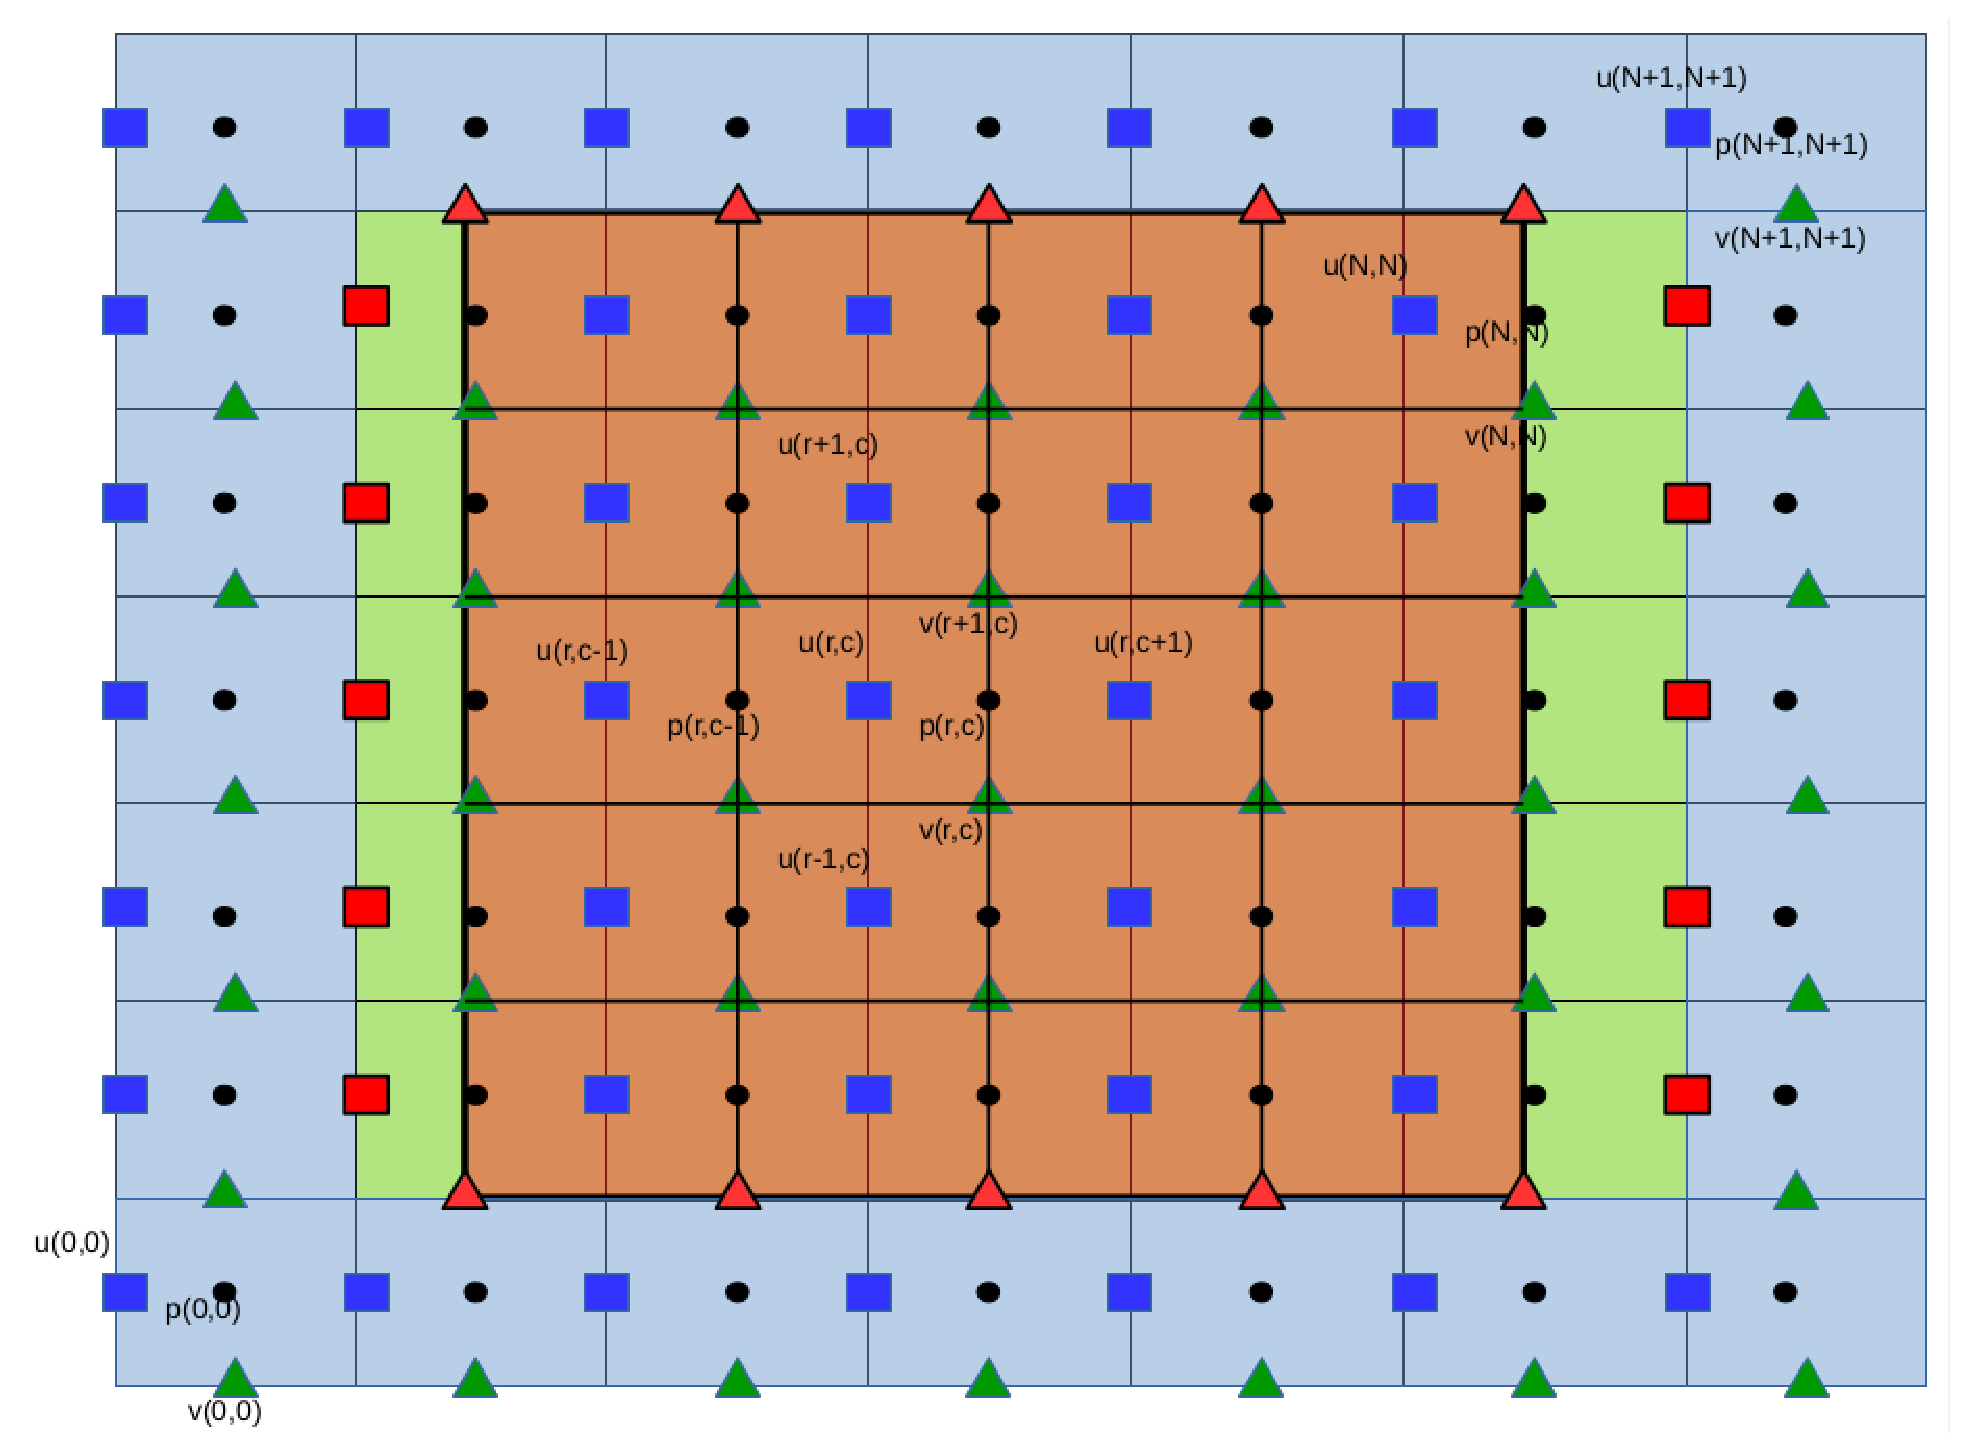
\includegraphics[width=0.8\textwidth]{xvel_calc.eps}
%       }	\\
% \subfloat[Staggered grid for calculation of y-velocity ]{%
%       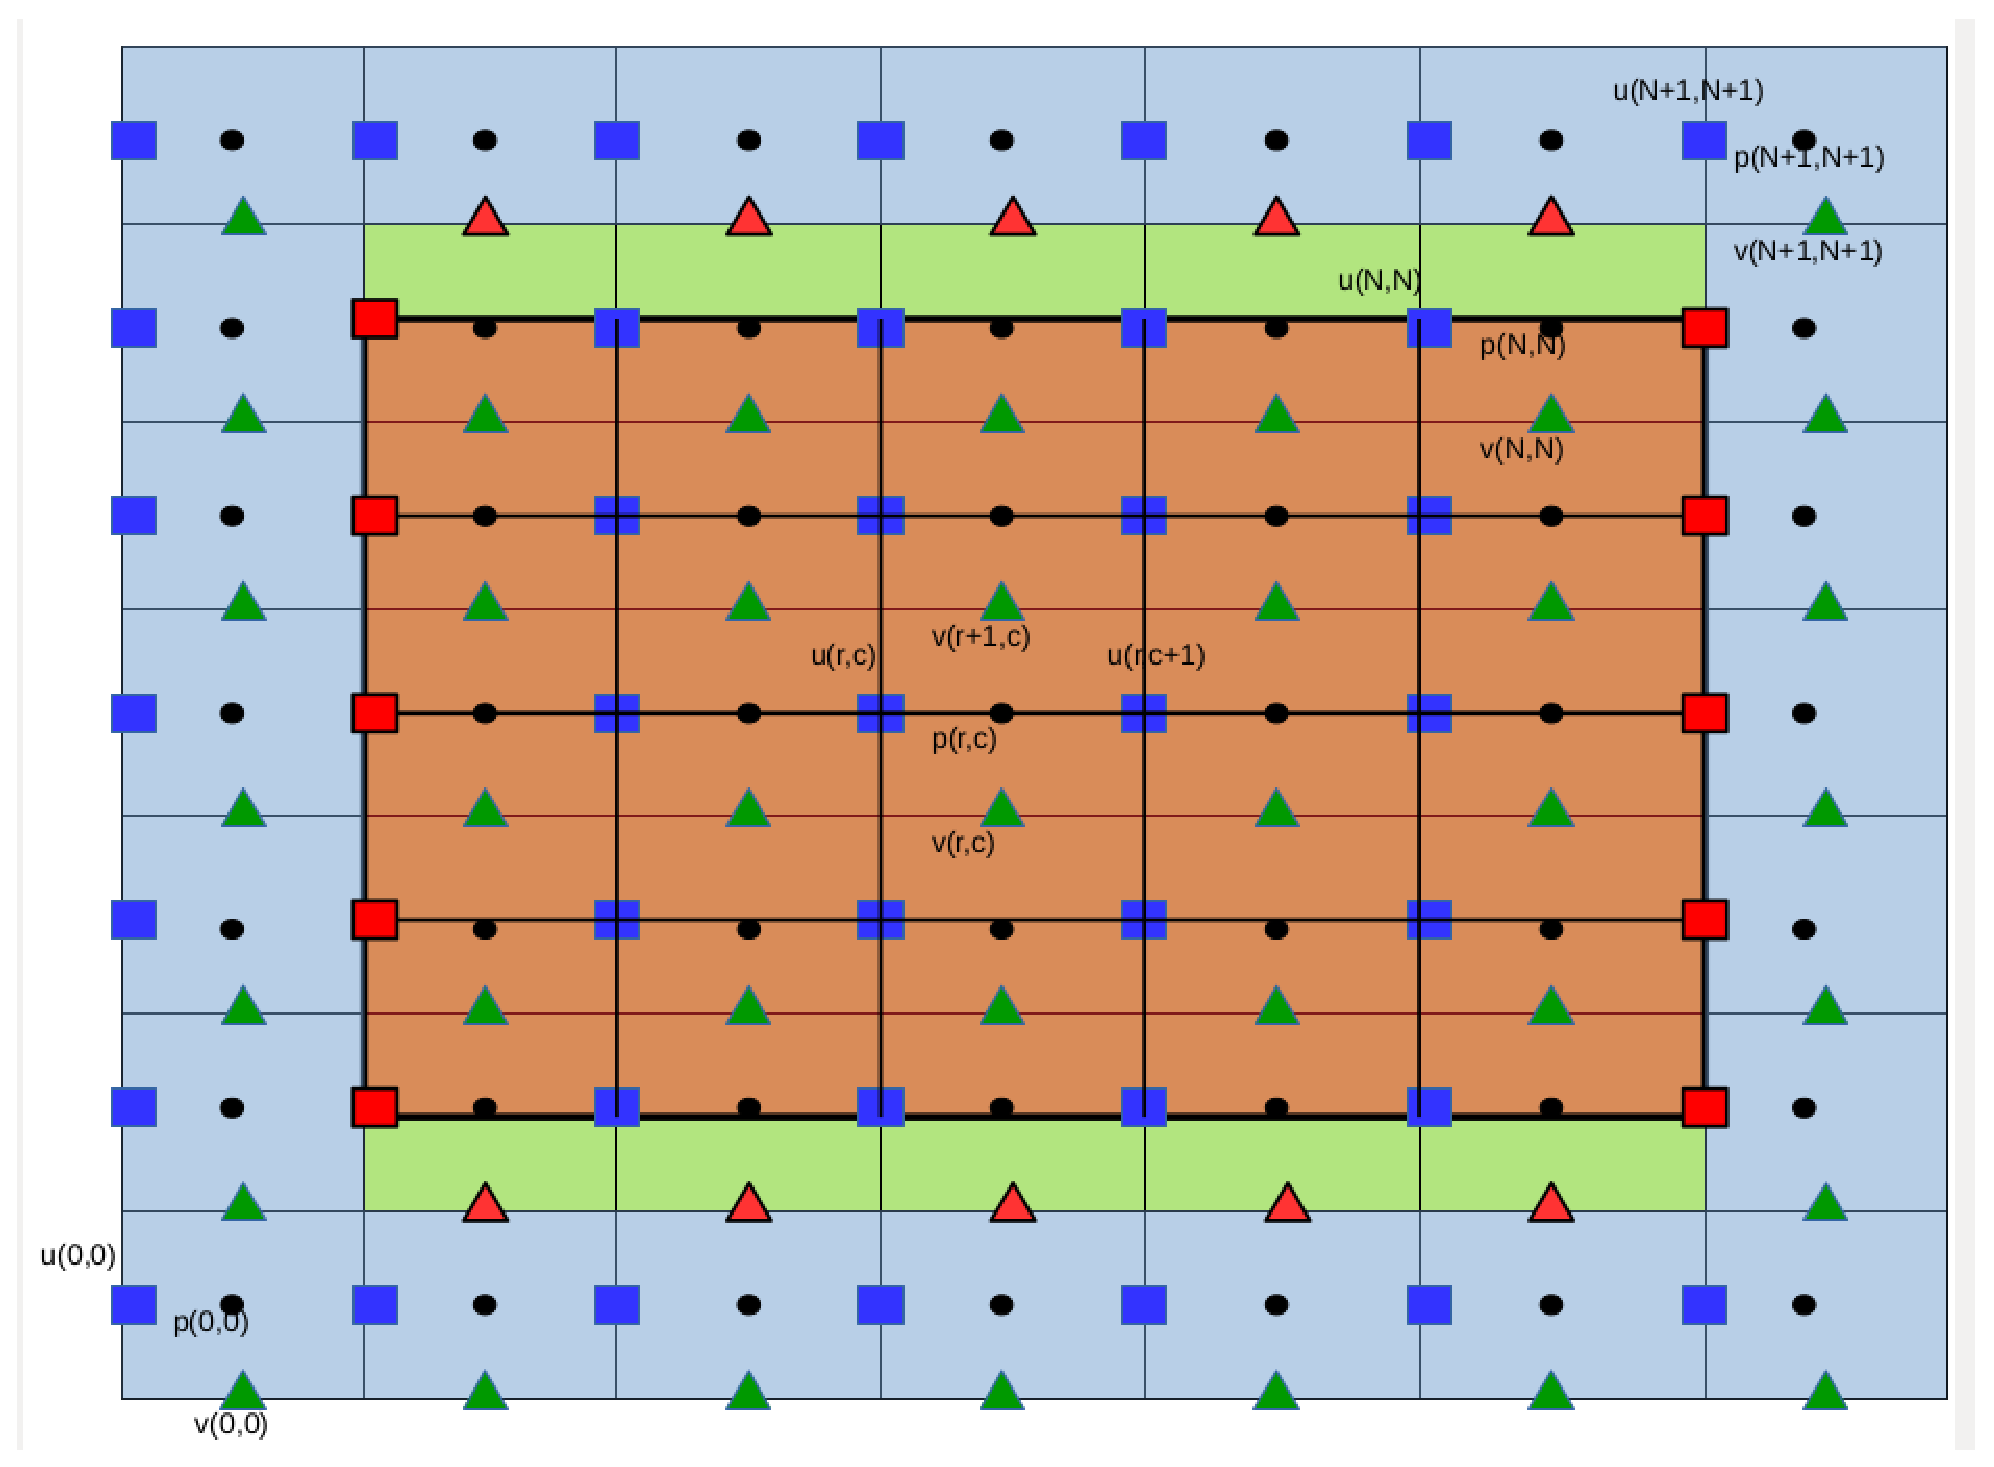
\includegraphics[width=0.8\textwidth]{yvel_calc.eps}
%       }
%       \caption{Different Computational grids for x and y velocity}
% \end{figure}
\subsubsection{Dirichlet Boundary Conditions}
The most commonly used boundary condition is the no-slip on the boundaries, we can set the velocity variables on the boundary to zero or any other value. On the left boundary of the 
domain, the x-velocities are defined so we can set them zero directly, but to set y-velocities we set the ghost control volumes y-velocities to change so that the average of ghost and 
the boundary control volume value becomes zero which is at the wall. This has to implemented inside the time loop, and ghost value has to be updated at every time step 

\begin{equation*}
 \boxed {\begin{align}
  v_{wall} &= \frac{v_{r,0}+v_{r,1}}{2} \\
 v_{r,0}&= 2v_{wall}-v_{r,1}
 \end{align} }
\end{equation*}

The similar operation is used for x-velocities at bottom and top boundaries.

\subsubsection{Neumann Boundary Conditions}
\label{sec:bc}
Conditions are where normal derivative for tangential component of velocity on the wall is zero, and normal component of
velocity on the wall is zero. This is equivalent to free slip, impermeable boundary, also called as symmetry condition. Mathematically, for left wall
\begin{equation*}
 \boxed{ \begin{align}
\frac{\partial v}{\partial x} = 0 \qquad\text{Neumann} \\
 u_{wall} = 0	\qquad\text{Dirichlet}
 \end{align} }
\end{equation*}
To implement the above Neumann condition, on say left wall, we set the following in our code,
\begin{equation*}
 \boxed{ v_{r,0}= v_{r,1} }
\end{equation*}
  
  \section{Pressure Poisson Equation(PPE)}
  For incompressible fluids, it can be followed from \ref{Eq:6} that,
  \begin{equation}
 \nabla .u^{n+1} = 0
 \label{Eq:35}
\end{equation}
\begin{equation*}
\begin{align}
  \nabla \cdot u^{n+1} = \nabla \cdot \left(u^*-\frac{\Delta t}{V}\int_V\frac{1}{\rho}\nabla  p^{n+1} dV\right) = 0 \\
 \nabla \cdot \left(\frac{\Delta t}{V}\int_V\frac{1}{\rho}\nabla  p^{n+1} dV\right) = \nabla \cdot u^*
  \end{align}
\end{equation*}

  \begin{equation}
 \frac{u_{r,c+1}^{n+1}-u_{r,c}^{n+1}}{\Delta x} + \frac{v_{r+1,c}^{n+1}-v_{r,c}^{n+1}}{\Delta y} = 0
\end{equation}
It essentially states that, any solution of velocity field should comply mass conservation, and the velocity field thus obtained must be divergence free. 
substituting (33) in (46), we get

\begin{eqnarray*}
 \frac{1}{\Delta x}\left[u_{r,c+1}^*-\frac{2\Delta t }{(\rho_{r,c}+\rho_{r,c+1})}\left(\frac{p_{r,c+1}-p_{r,c}}{\Delta x}\right) \right.	\\
- \left. u_{r,c}^*+\frac{2\Delta t }{(\rho_{r,c}+\rho_{r,c-1})}\left(\frac{p_{r,c}-p_{r,c-1}}{\Delta x}\right)\right]	\\
+\frac{1}{\Delta y}\left[v_{r+1,c}^*-\frac{2\Delta t }{(\rho_{r+1,c}+\rho_{r,c})}\left(\frac{p_{r+1,c}-p_{r,c}}{\Delta y}\right) \right.	\\
-\left. v_{r,c}^*+\frac{2\Delta t }{(\rho_{r,c}+\rho_{r-1,c})}\left(\frac{p_{r,c}-p_{r-1,c}}{\Delta y}\right)\right]	=0
\end{eqnarray*}
From which we obtain,
 \begin{eqnarray*}
p_{r,c} = \left[\frac{1}{(\Delta x)^2}\left(\frac{1}{\rho_{r,c+1}+\rho_{r,c}}+\frac{1}{\rho_{r,c}+\rho_{r,c-1}}\right)
+\frac{1}{(\Delta y)^2}\left(\frac{1}{\rho_{r+1,c}+\rho_{r,c}}+\frac{1}{\rho_{r,c}+\rho_{r-1,c}}\right)\right]^{-1} \\
\left\{\frac{1}{(\Delta x)^2}\left(\frac{p_{r,c+1}}{\rho_{r,c+1}+\rho_{r,c}}+\frac{p_{r,c-1}}{\rho_{r,c}+\rho_{r,c-1}}\right)\right.
\left.+\frac{1}{(\Delta y)^2}\left(\frac{p_{r+1,c}}{\rho_{r+1,c}+\rho_{r,c}}+\frac{p_{r-1,c}}{\rho_{r,c}+\rho_{r-1,c}}\right)\right. \\
-\frac{1}{2\Delta t}\left. \left(\frac{u_{r,c+1}^*-u_{r,c}^*}{\Delta x} +\frac{v_{r+1,c}^*-v_{r,c}^*}{\Delta y}\right)\right\}
 \end{eqnarray*}

\subsection{Successive Over Relaxation method (SOR)}
Successive over relaxation method is used to solve a linear system of equations derived by extrapolating the Gauss-Sidel method. This extrapolation 
takes the form of a weighted average between the previous iterate and the computed Gauss-Seidel iterate successively for each component.
\begin{eqnarray*}
 y_i^k = \omega \overline{y}_i^k + (1-\omega)y_i^{k-1} 
\end{eqnarray*}
where $\overline{y}_i^k$, denotes the Gauss-Sidel iterate and $\omega$ is the relaxation parameter which is used to accelerate the convergence.
\begin{eqnarray*}
 p_{r,c}^{\alpha+1} = \omega \left[\frac{1}{(\Delta x)^2}\left(\frac{1}{\rho_{r,c+1}+\rho_{r,c}}+\frac{1}{\rho_{r,c}+\rho_{r,c-1}}\right)
+\frac{1}{(\Delta y)^2}\left(\frac{1}{\rho_{r+1,c}+\rho_{r,c}}+\frac{1}{\rho_{r,c}+\rho_{r-1,c}}\right)\right]^{-1} \\
\left\{\frac{1}{(\Delta x)^2}\left(\frac{p_{r,c+1}}{\rho_{r,c+1}+\rho_{r,c}}+\frac{p_{r,c-1}}{\rho_{r,c}+\rho_{r,c-1}}\right)\right.
\left.+\frac{1}{(\Delta y)^2}\left(\frac{p_{r+1,c}}{\rho_{r+1,c}+\rho_{r,c}}+\frac{p_{r-1,c}}{\rho_{r,c}+\rho_{r-1,c}}\right)\right. \\
-\frac{1}{2\Delta t}\left. \left(\frac{u_{r,c+1}^*-u_{r,c}^*}{\Delta x} +\frac{u_{r,c+1}^*-u_{r,c}^*}{\Delta x}\right)\right\}\\
+(1-\omega)p_{r,c}^{\alpha}
\end{eqnarray*}

where $\alpha$ is the previous iteration step and $\omega$ is the relaxation parameter, which can take values from 0-2, for overrelaxation it must be greater than 1.
For stability reasons it must be below 2. A choice of $\omega= 1.2 -1.5$ is usually a good compromise between stability and convergence. The advantage to use SOR is its simplicity 
but it converges very slowly. For faster runs we have to more use advanced methods. (\cite{Tryggvason2011})

\subsection{Boundary Conditions for PPE}
There is no explicit boundary condition for pressure needed, rather we use velocity boundary conditions to get pressure at boundary control volumes. (\cite{Tryggvason2011})
thus \ref{Eq:35} at boundary reduces to 
  \begin{equation}
 \frac{u_{r,c+1}^{n+1}-u_{b,r}}{\Delta x} + \frac{v_{r+1,c}^{n+1}-v_{r,c}^{n+1}}{\Delta y} = 0
 \label{Eq:37}
\end{equation}
where $u_{b,r}$, the boundary value of velocity is known by velocity boundary conditions. From \ref{Eq:37}  the $p_{r,c}$ is computed on the boundary and corner control volumes.
   
\section{Coupling VOF and Navier-Stokes solver}
The volume of fluid interface capturing is coupled with the Navier-stokes solver. Figure \ref{Fig:coupling} shows the schematic to couple the interface capturing and Navier-stokes
solver for a time step. The steps followed are discussed in detail below:-
\begin{figure}
 \centering
 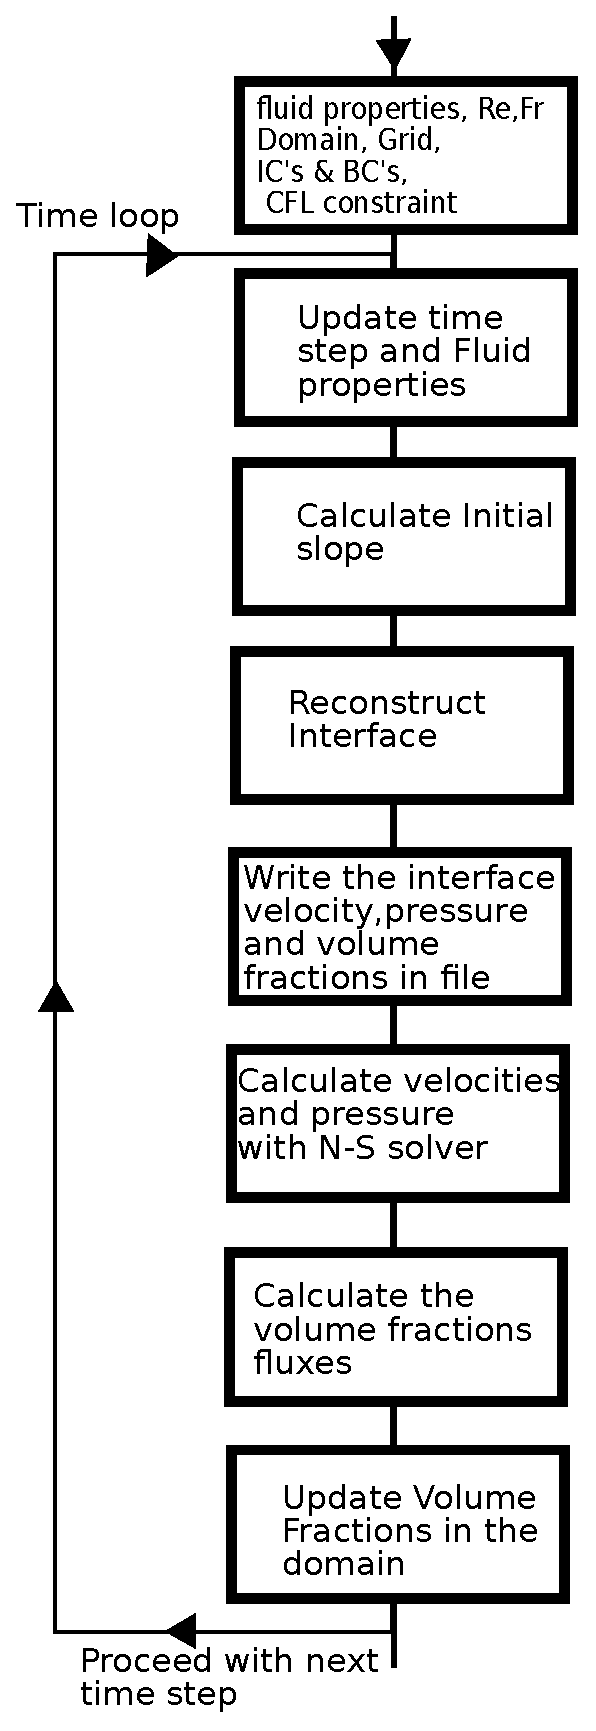
\includegraphics[scale=0.5]{coupling.eps}
 \caption{Sequence to couple VOF and N-S solver}
 \label{Fig:coupling}
\end{figure}

\underline{Input}\\
The solver is fed with following to start the time marching:-
\begin{enumerate}
 \item Initial Volume Fraction field which described the initial condition of the interface
 \item Density ratio of light to the dark fluid, $\tilde\mu = \frac{\rho_G}{\rho_L}$ %($F_{light}=0 \qquad F_{dark}=1$)
 \item Viscosity ratio of light to dark fluid, $\tilde\mu = \frac{\mu_G}{\mu_L}$
 \item Reynolds number defined with dark fluid scales $Re = \frac{Lu\rho_L}{\mu_L}$
 \item CFL number
 \item Domain size
 \item Mesh - No of Cells
\end{enumerate}
\underline{Update time step and fluid properties}\\
The time step is varied to follow the CFL criteria to keep the advection scheme numerically stable. The time step is calculated by
\begin{equation}
 \Delta t = CFL\left(\frac{\Delta}{2u_{max}}\right)
\end{equation}
where $u_{max}$ is the maximum velocity in the actual domain. CFL number should be less than 1.\\
The fluid properties i.e. density $\tilde\rho$, and viscosity $\tilde\mu$ field is updated at every time step using the volume fraction field, which describes the properties
of the fluid in the cells where velocities has to be computed.
\begin{eqnarray}
 \rho_{r,c} = F + (1-F)\tilde\rho  \nonumber \\
 \mu_{r,c} = F + (1-F)\tilde\mu 
\end{eqnarray}
\underline{Calculate Initial slope}\\
Initial guess is calculated using Green-Gauss gradient given by the Equation \ref{Eq:GG}\\
\underline{Reconstruct Interface}\\
Reconstruct the interface using the LVIRA in all the cells in the actual domain.\\
\underline{Write the data}\\
Following data is stored in a file at required intervals. This file can be used to restart the simulation and march further in time.
\begin{enumerate}
 \item x-velocity
 \item y-velocity
 \item Pressure
 \item Volume Fraction
\end{enumerate}
Interface information i.e. the coordinates of the lines in the domain is stored in a different file.\\
\underline{Calculate velocities}\\
The x and y velocities are calculated using the projection method as discussed above in this chapter.\\
\underline{Calculate the volume fraction fluxes}\\
The fluxes are calculated in all the cells actual domain using the velocity field calculated in previous step.\\
\underline{Update the volume fractions}\\
The volume fractions are updated using the fluxes calculated above and the proceed to next time step in the loop by updating the fluid properties with 
updated volume fractions.

\section{Verification}
The test problems were set without any surface tension model and compared with respective available data.
\subsection{Lid Driven Cavity test}
A problem was set test lid driven cavity to get a steady state solution. A square domain of unit length, single fluid and Reynolds number 100, 400, 1000.
The results are validated by \cite{Ghia1982}. Figure \ref{Fig:xyvel1000} shows the x-velocity along vertical center-line and y-velocity along horizontal center-line respectively in the domain. 
Stream function and vorticity contours are shown in Figure \ref{Fig:cont1000}.
\begin{figure}
\centering
  \subfloat[x-velocity along vertical centerline (Re=100) ]{%
      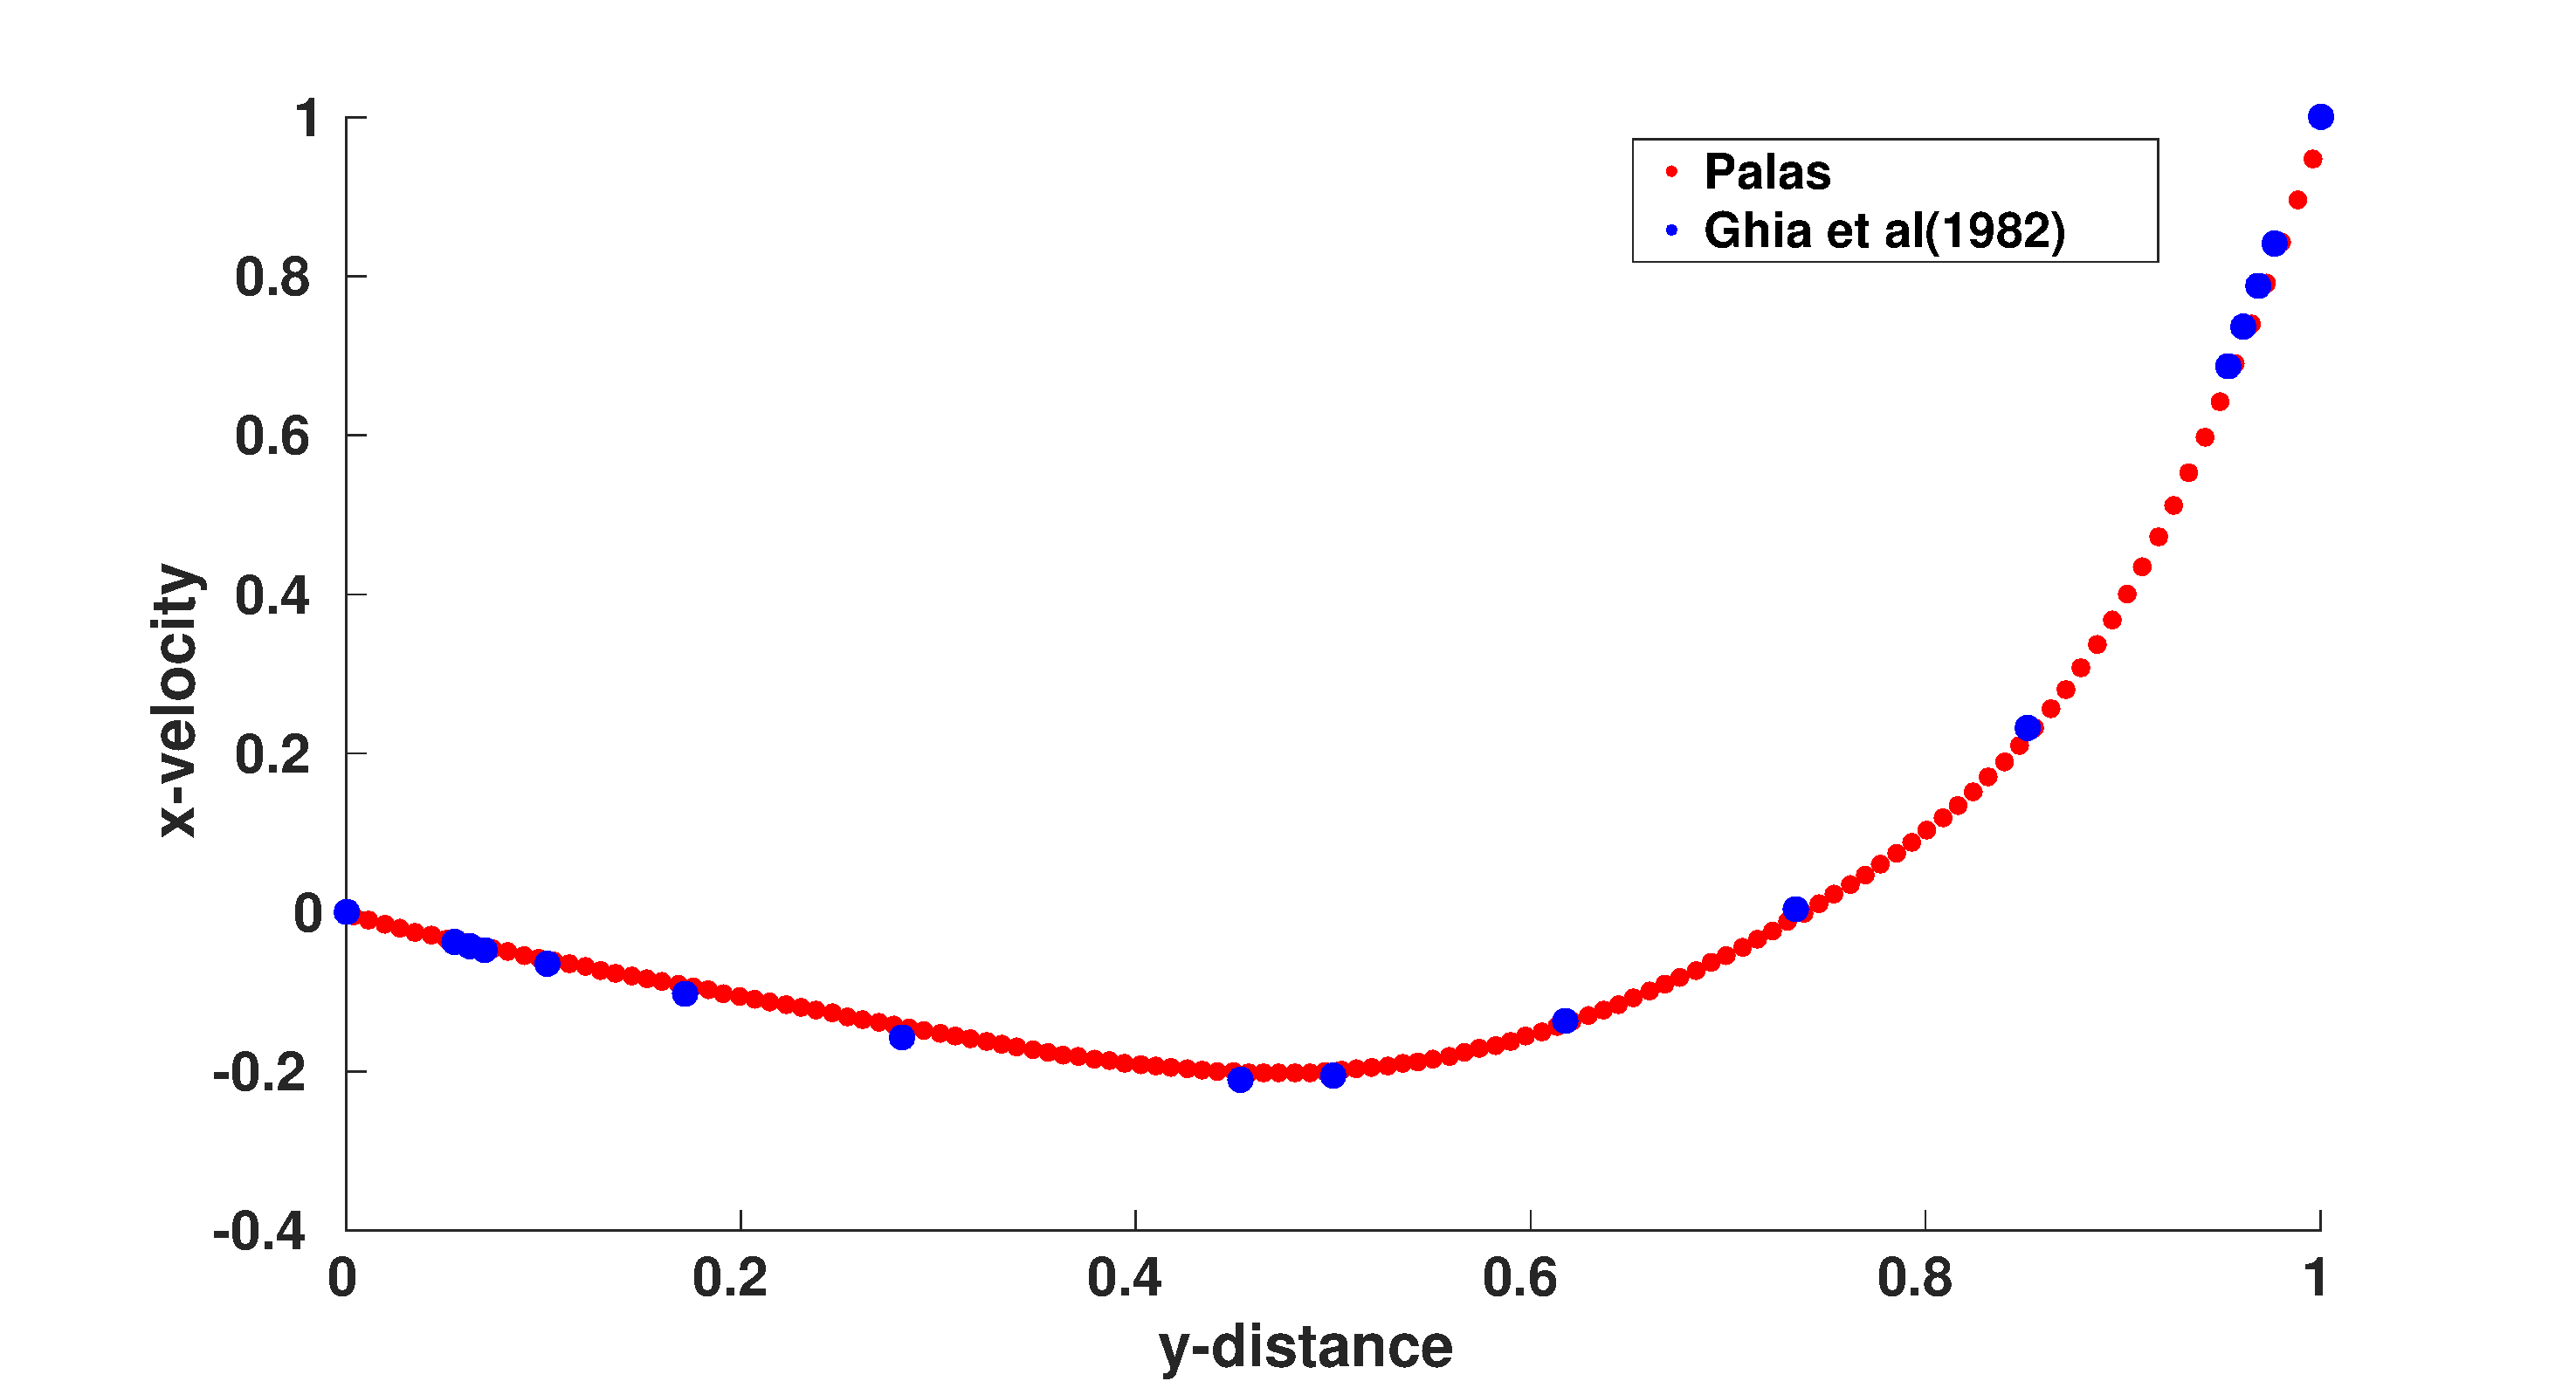
\includegraphics[width=0.5\textwidth]{Re100u.eps}
      }	
 \subfloat[y-velocity along horizontal centerline (Re=100) ]{%
      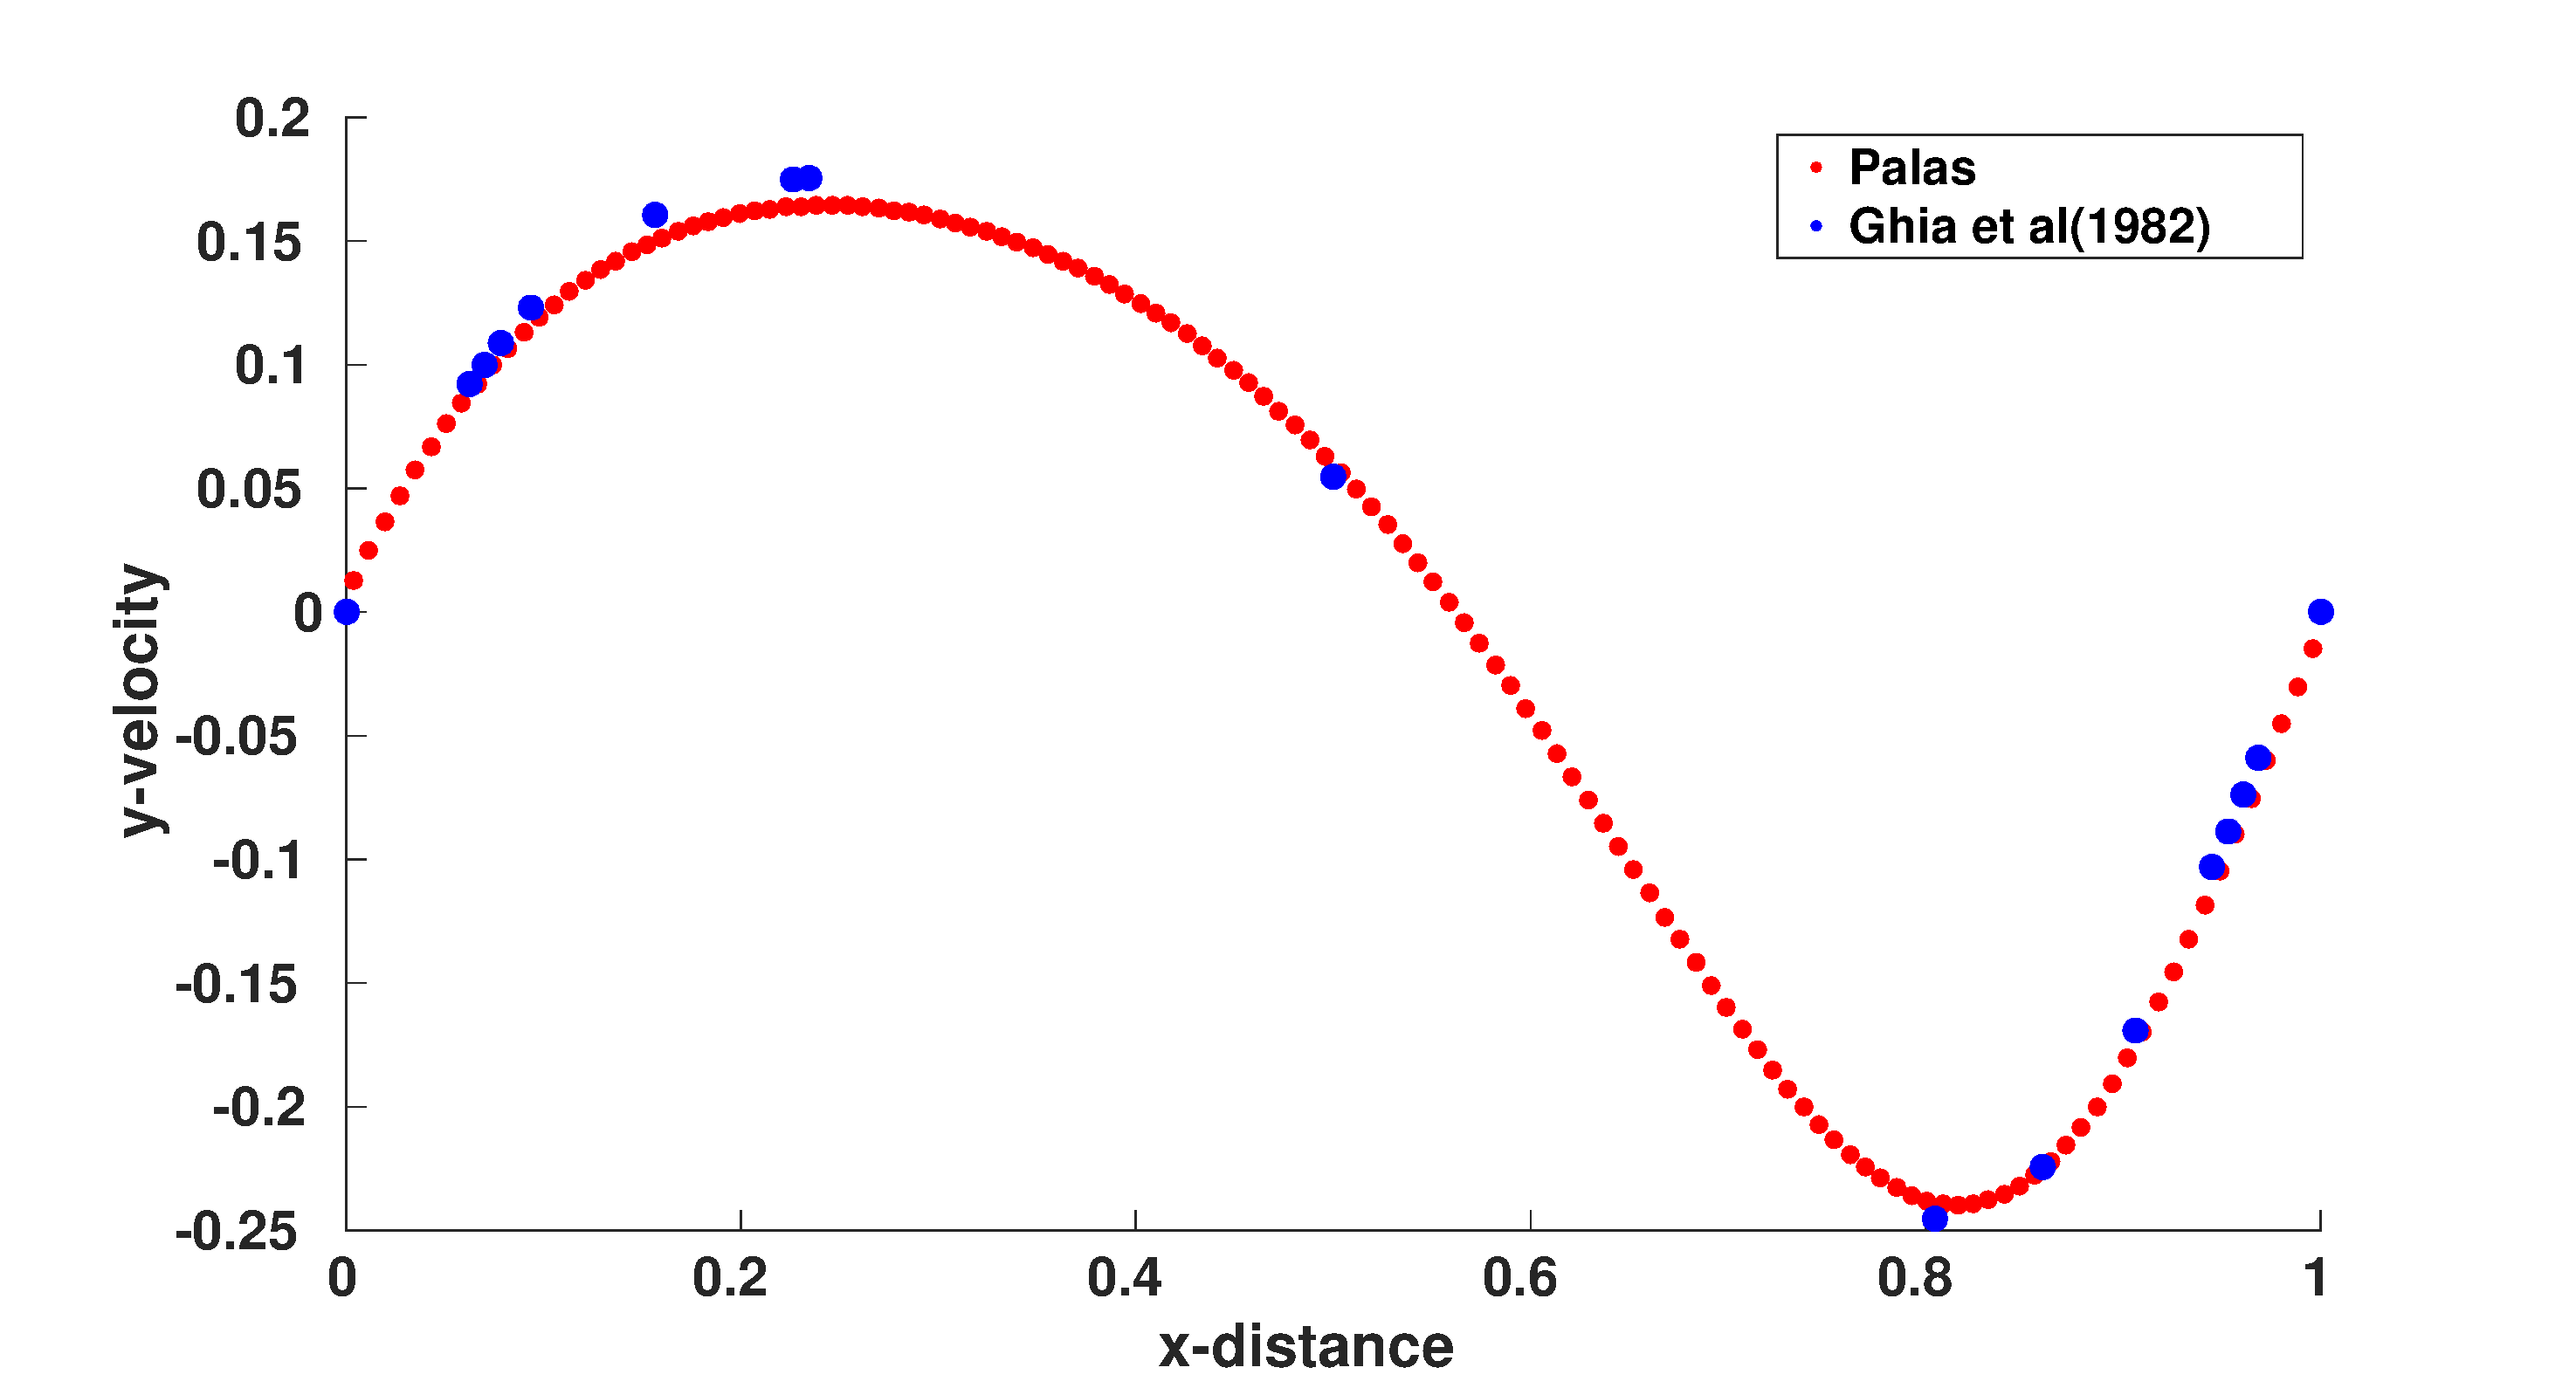
\includegraphics[width=0.5\textwidth]{Re100v.eps}
      }\\
  \subfloat[x-velocity along vertical centerline (Re=400) ]{%
      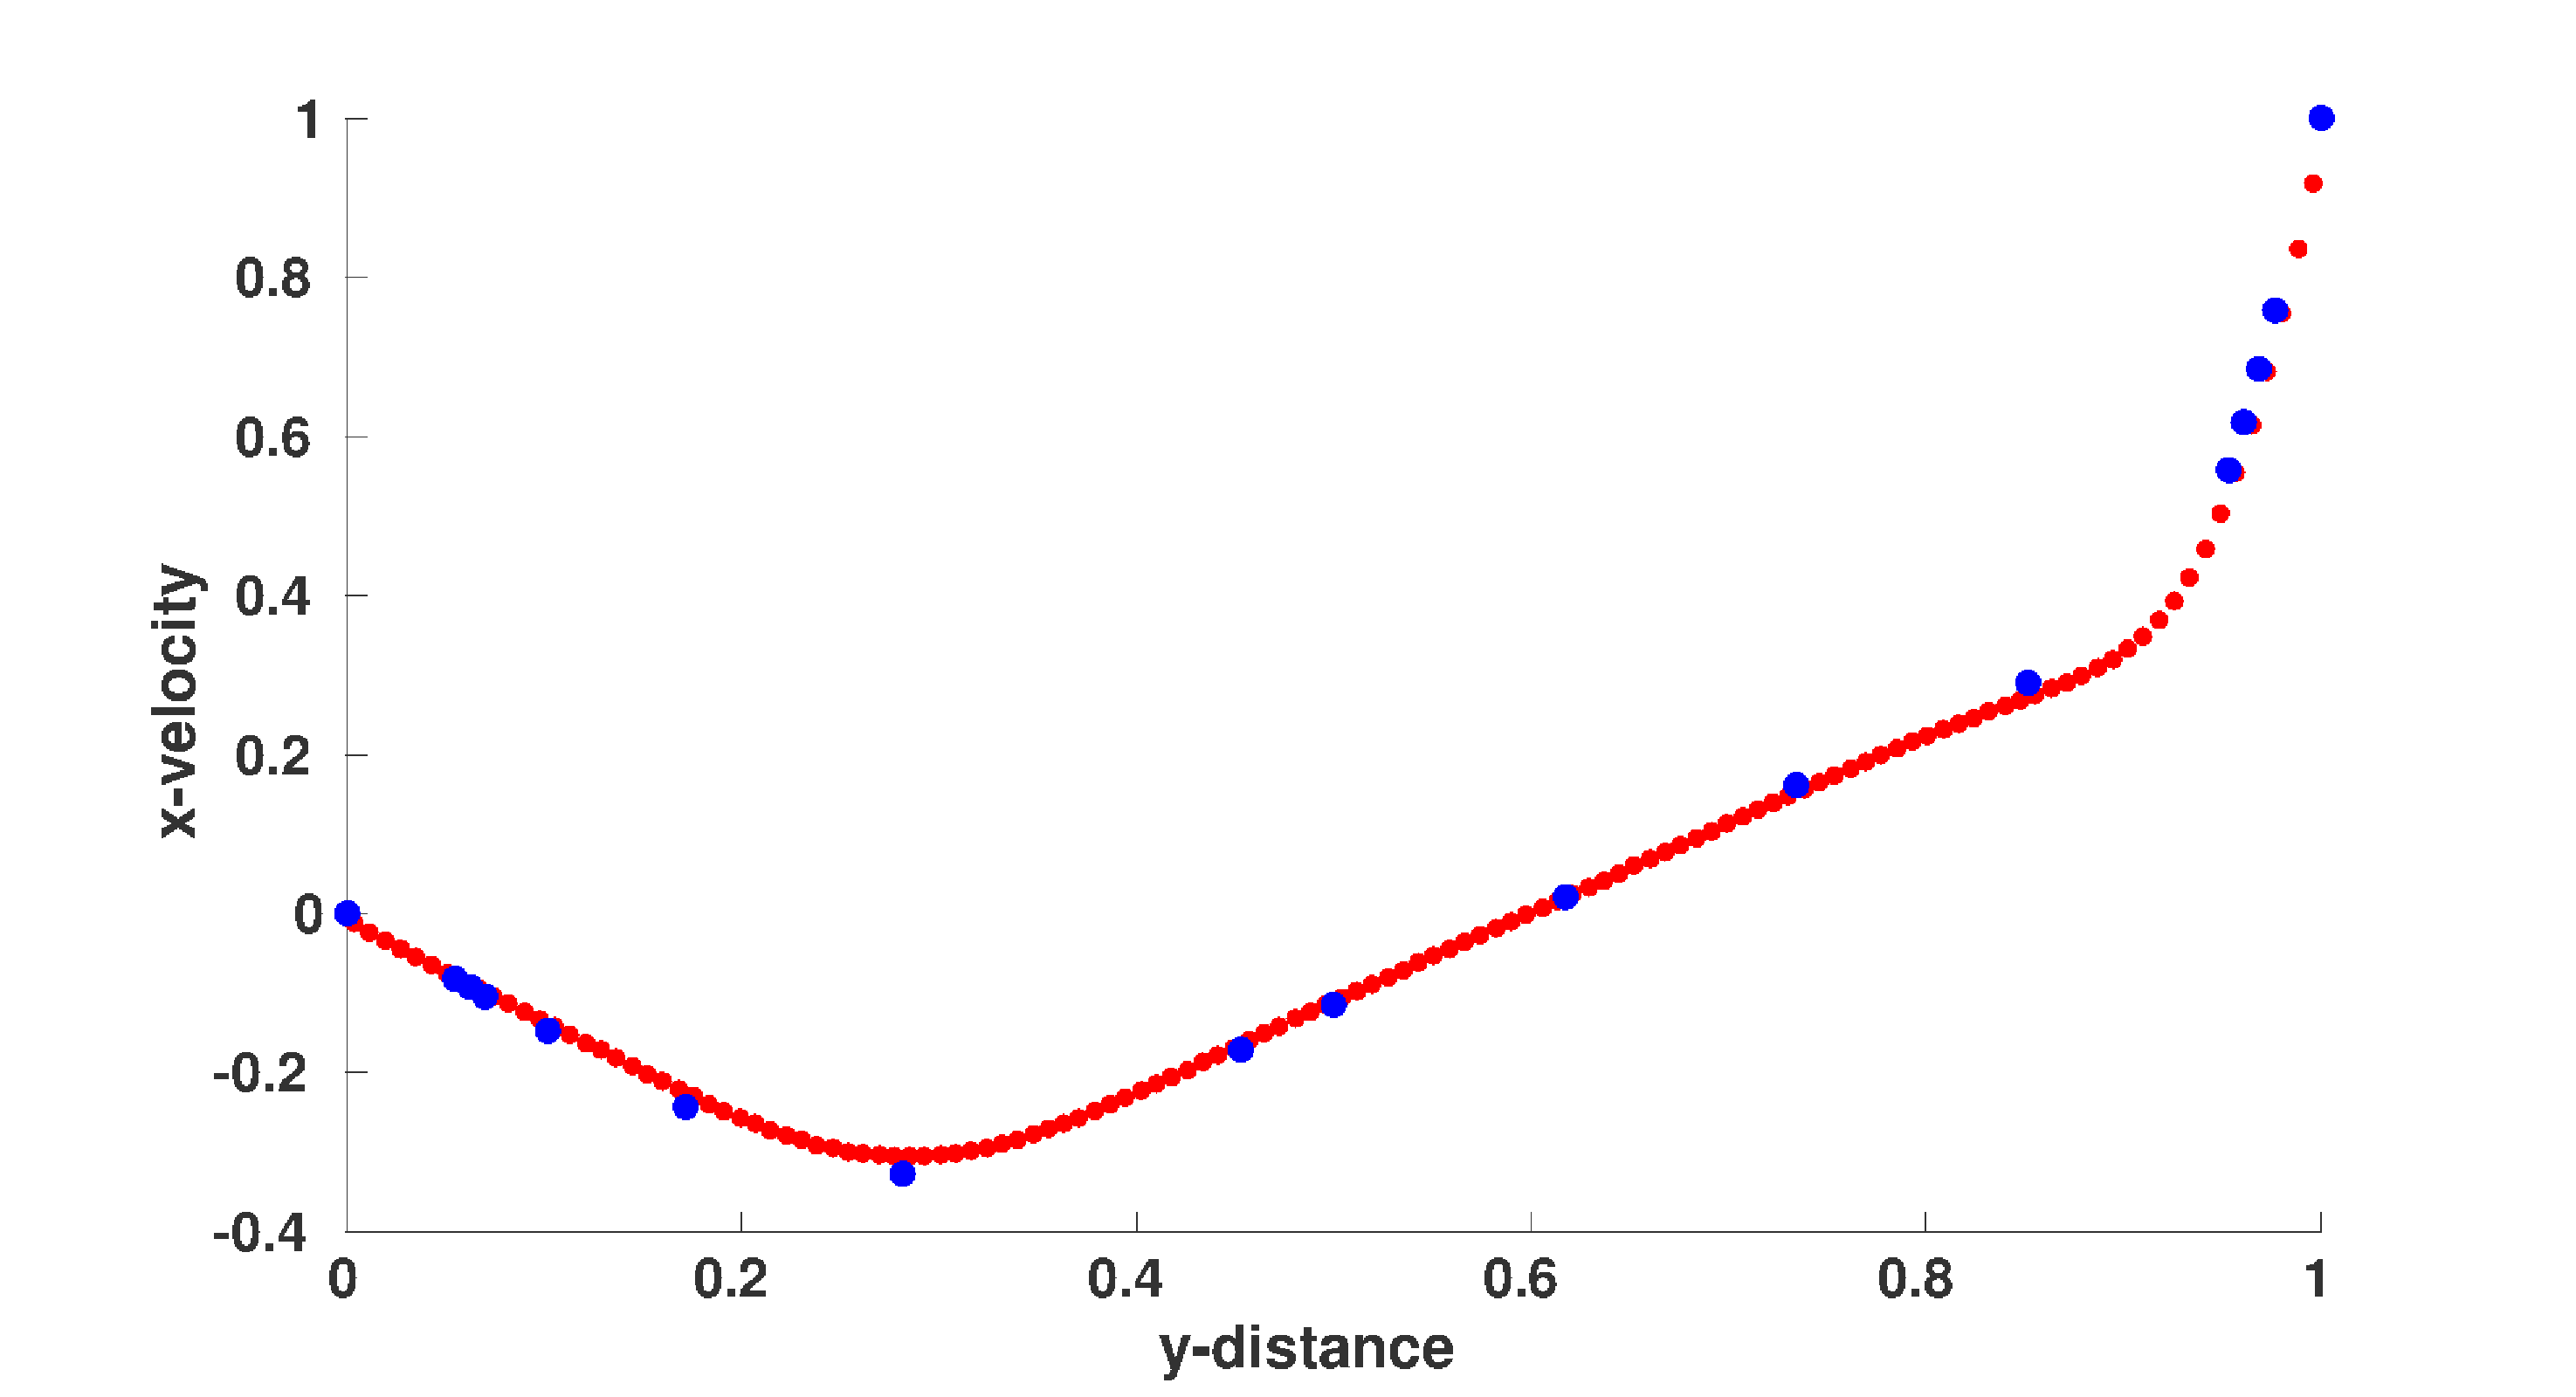
\includegraphics[width=0.5\textwidth]{Re400u.eps}
      }	
 \subfloat[y-velocity along horizontal centerline (Re=400) ]{%
      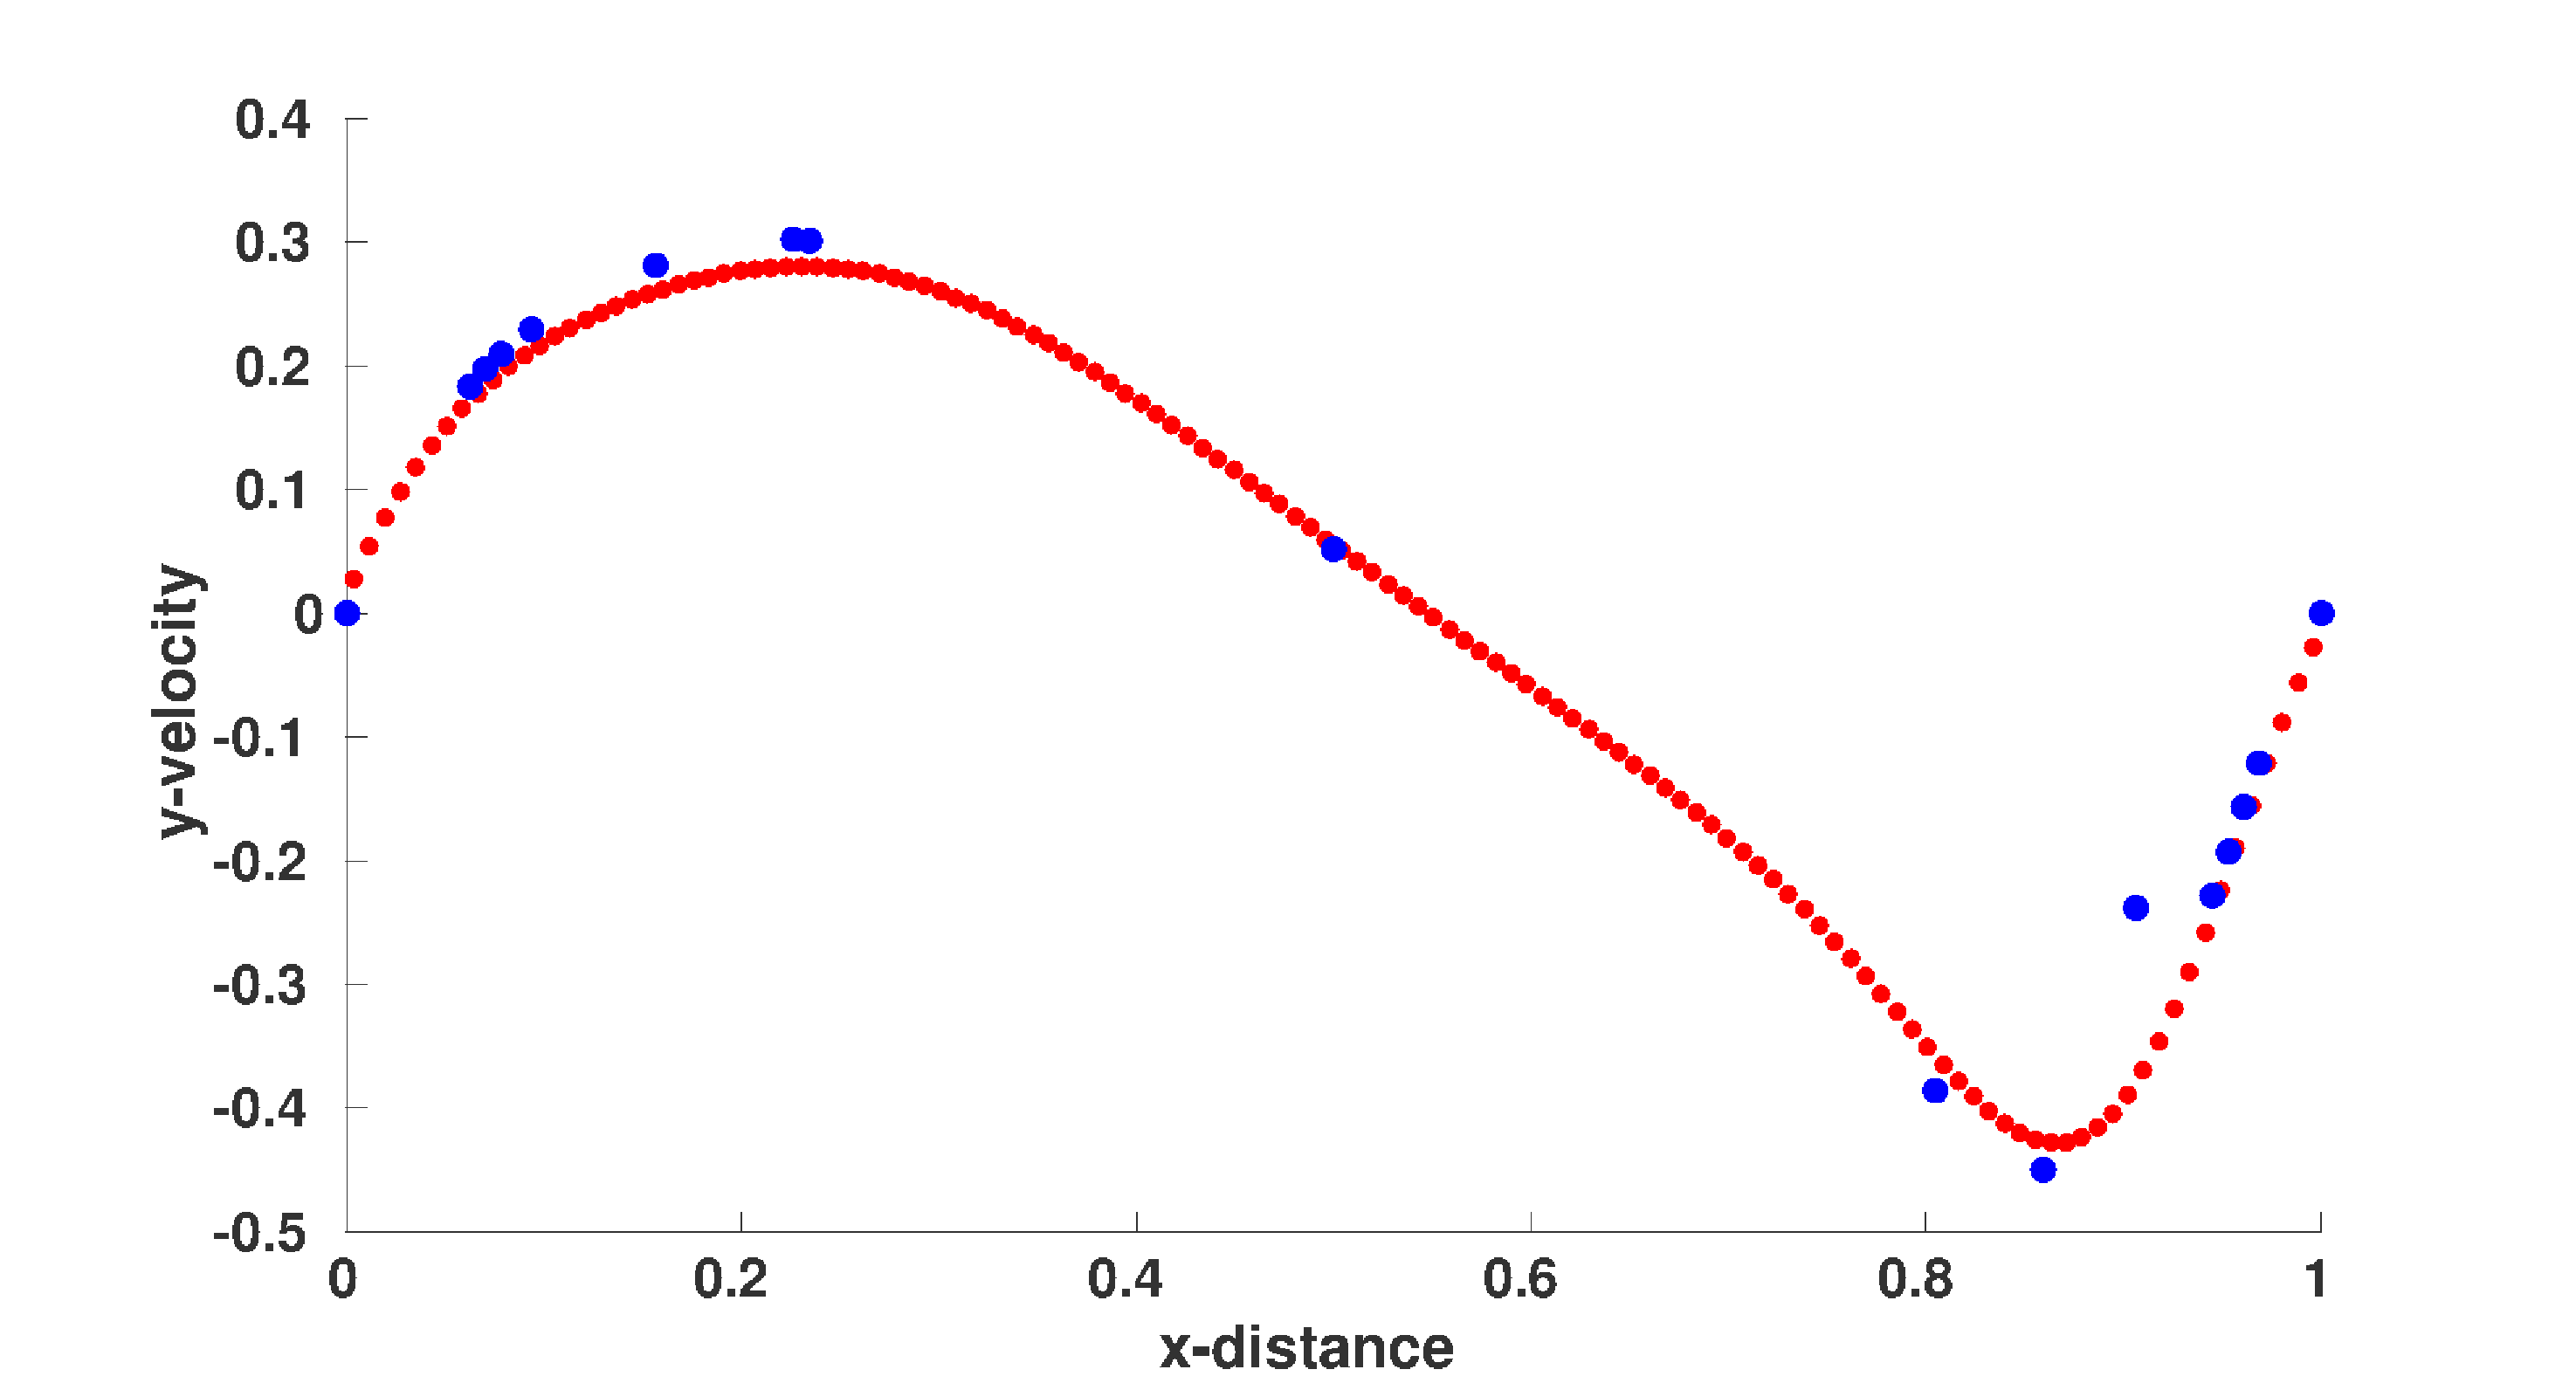
\includegraphics[width=0.5\textwidth]{Re400v.eps}
      }\\
  \subfloat[x-velocity along vertical centerline (Re=1000) ]{%
      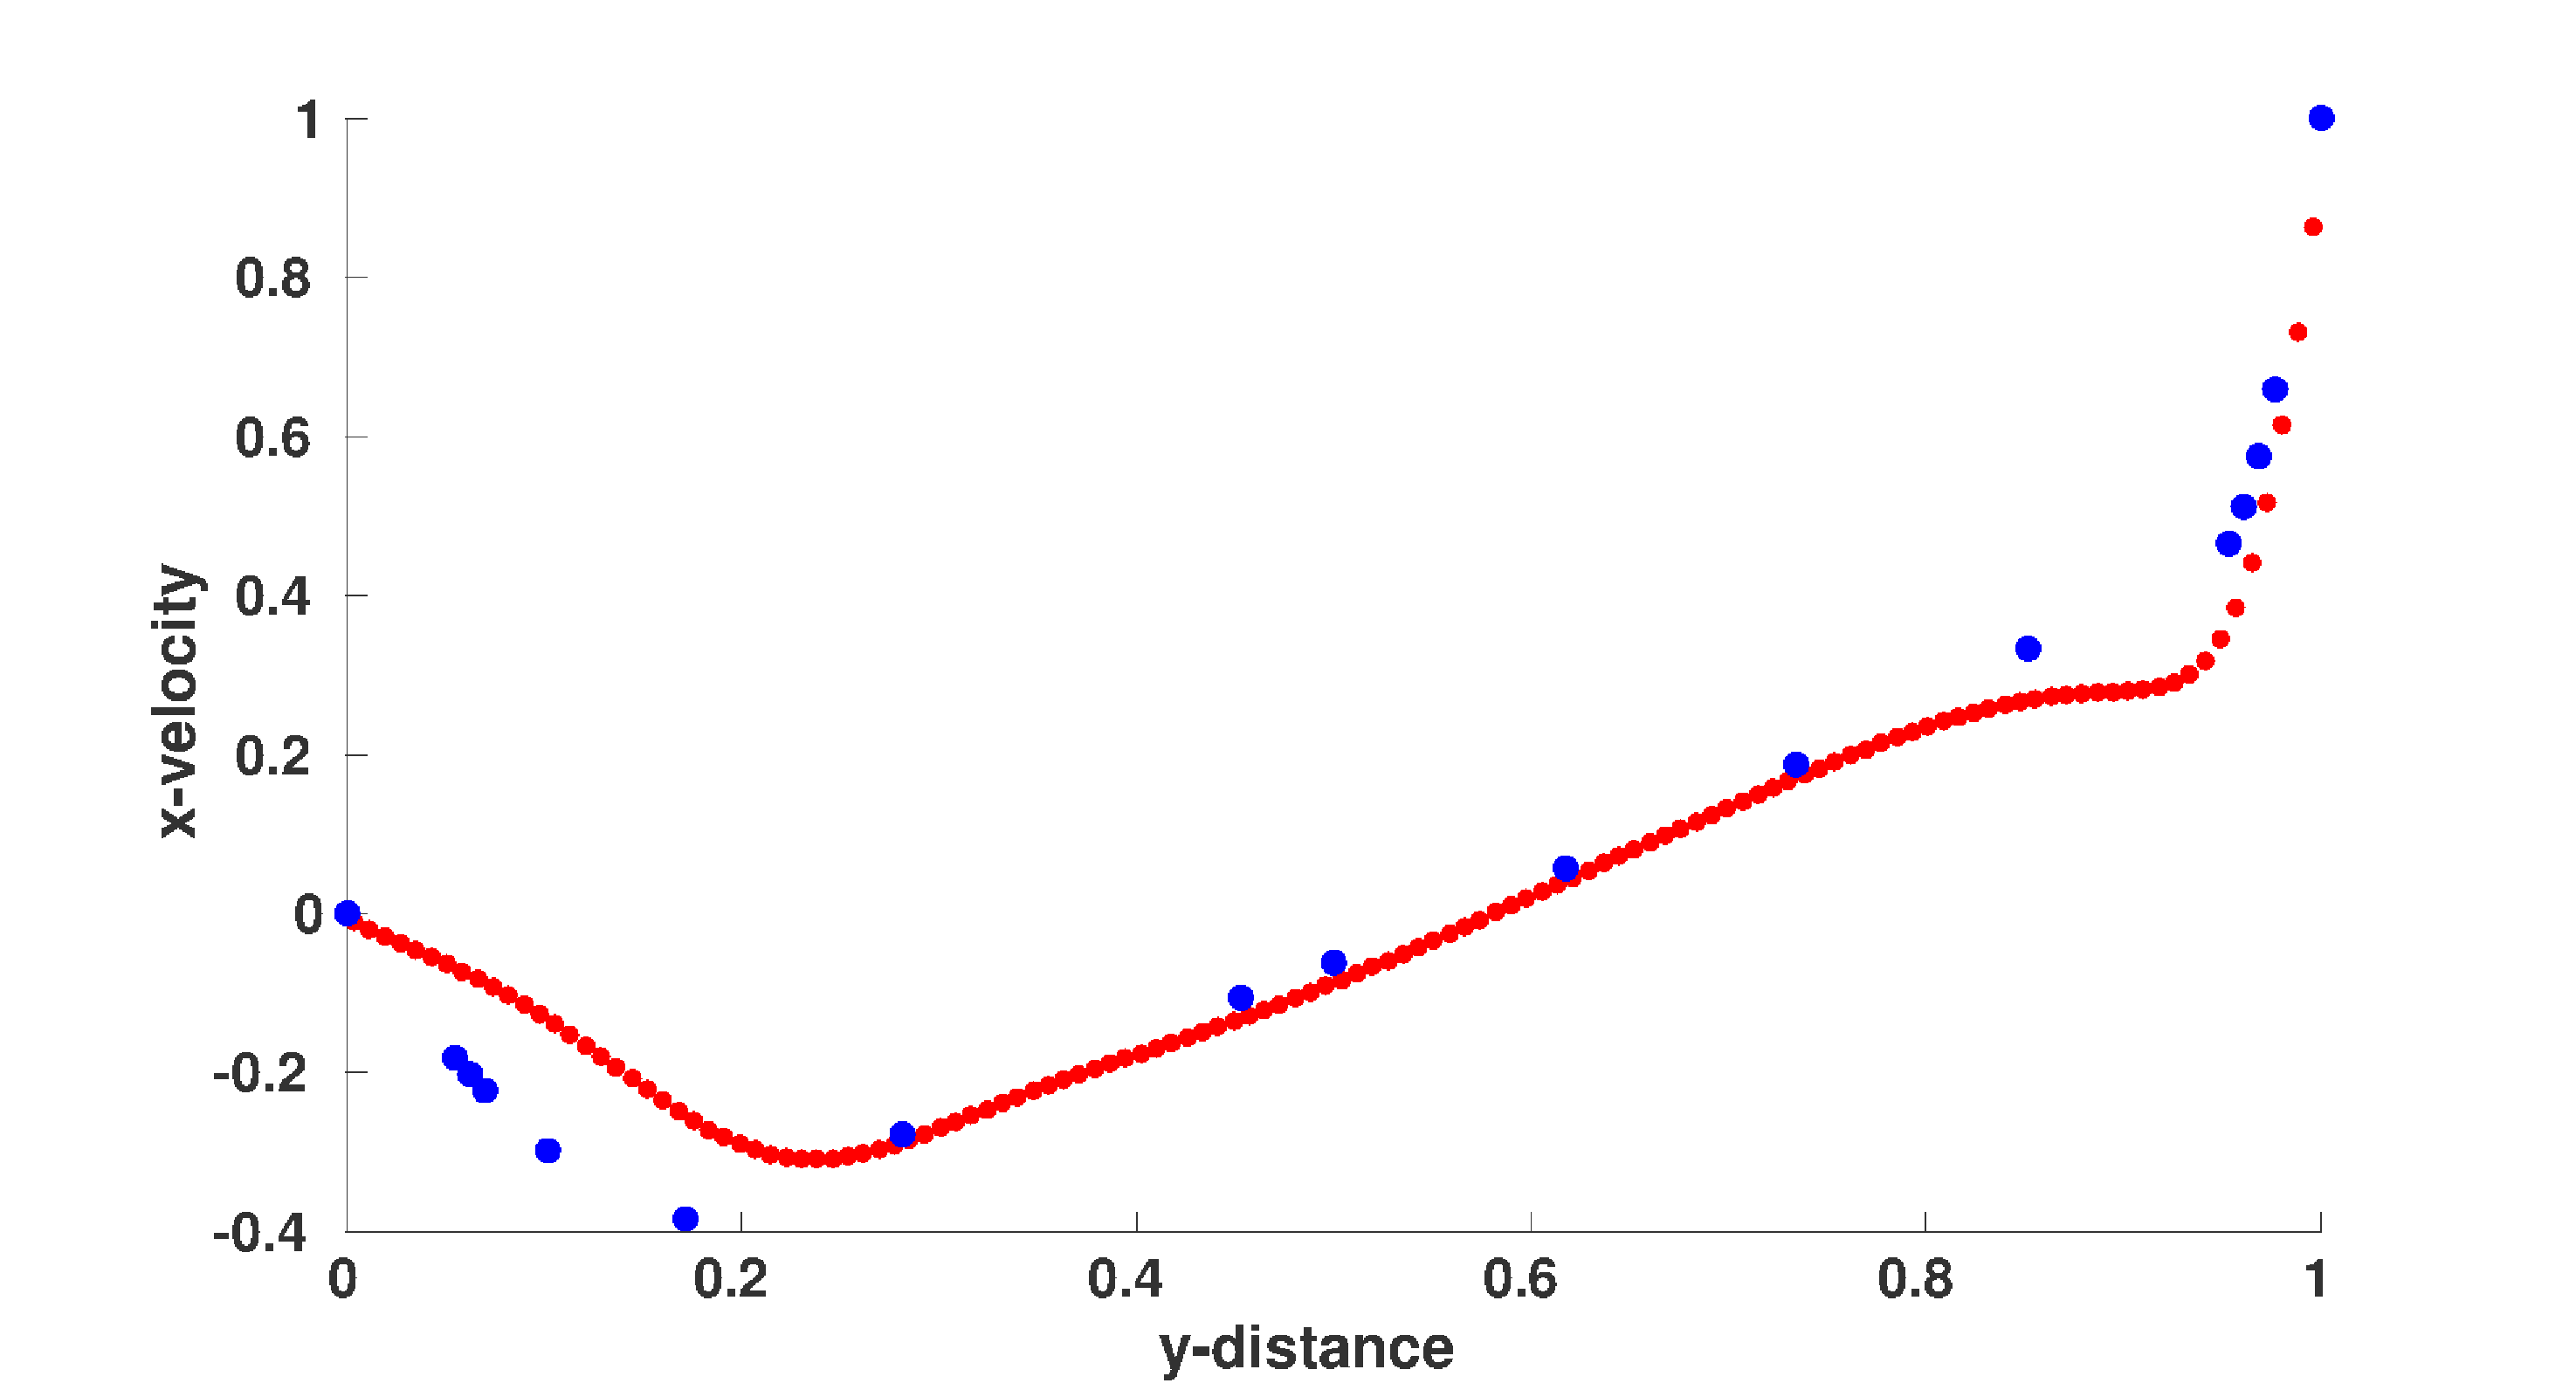
\includegraphics[width=0.5\textwidth]{Re1000u.eps}
      }	
 \subfloat[y-velocity along horizontal centerline (Re=1000) ]{%
      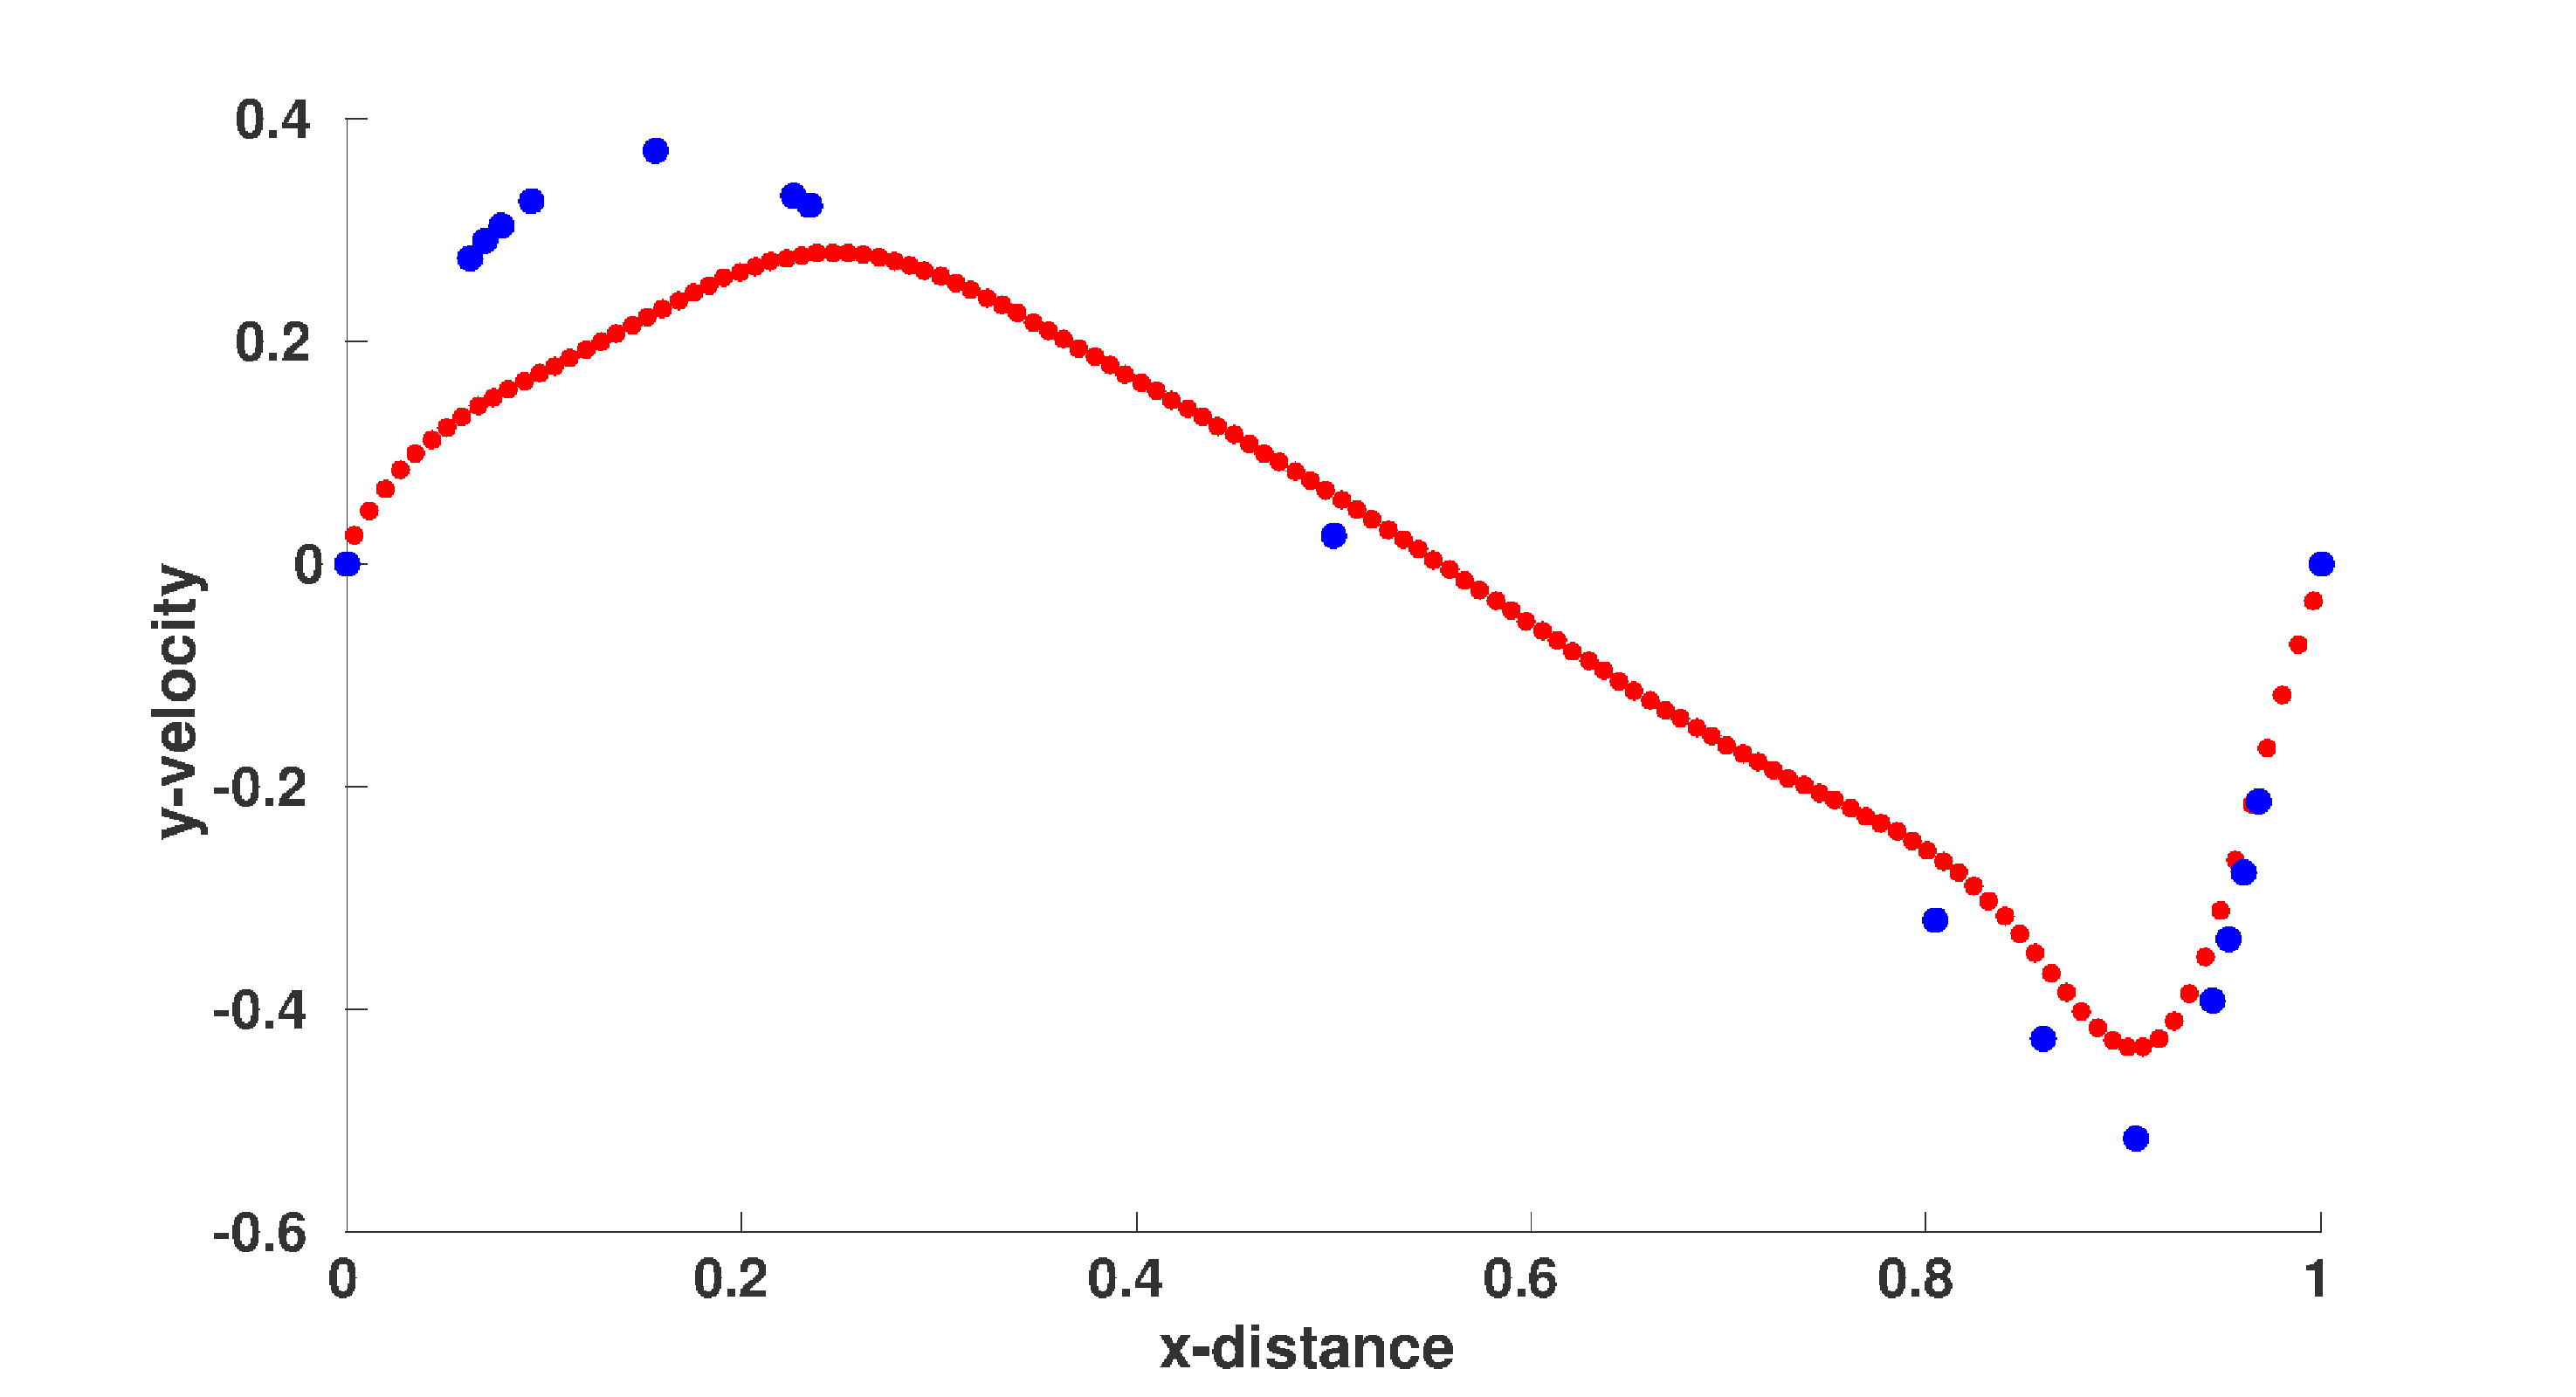
\includegraphics[width=0.5\textwidth]{Re1000v.eps}
      }
 \caption{Blue:\cite{Ghia1982}, Red:Present Study(LVIRA)}
 \label{Fig:xyvel1000}
\end{figure}

\begin{figure}
\centering
  \subfloat[Stream function contours at Re=100 ]{%
      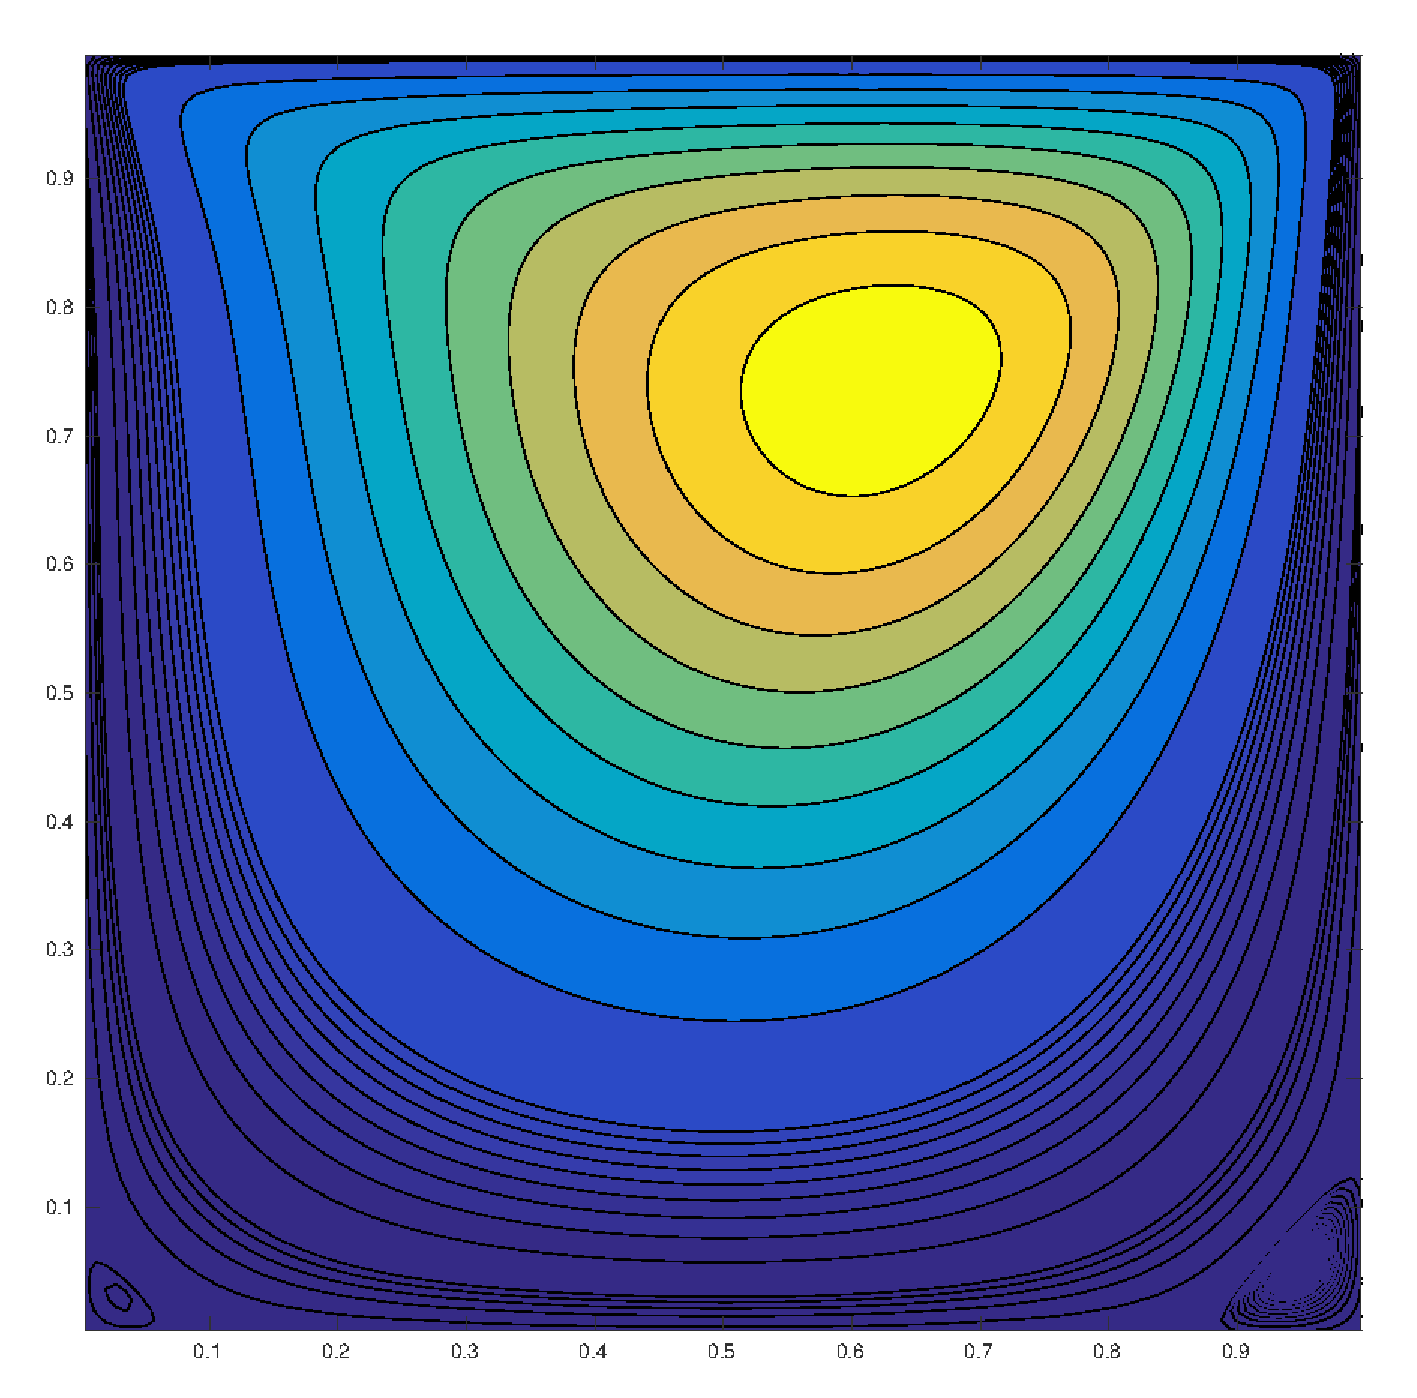
\includegraphics[width=0.4\textwidth]{Re100_streamf.eps}
      }	
 \subfloat[Vorticity contours at Re=100 ]{%
      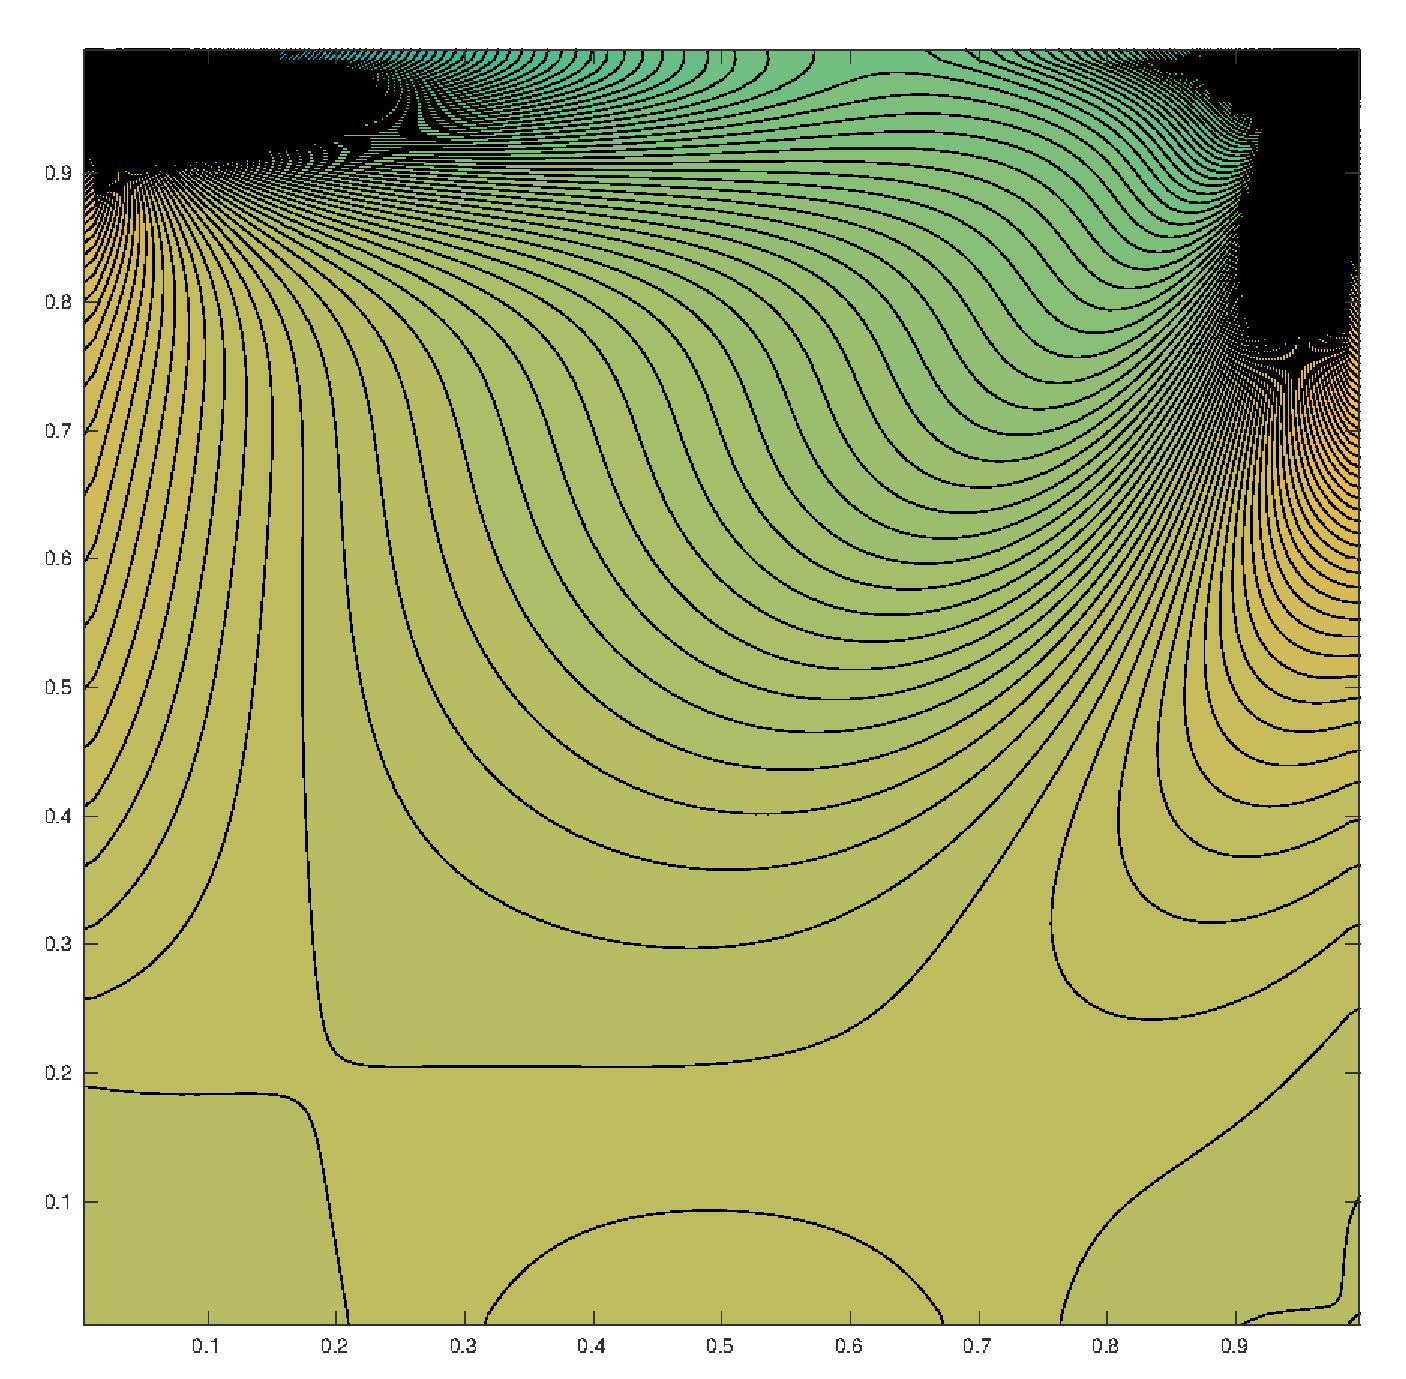
\includegraphics[width=0.4\textwidth]{Re100_vortf.eps}
      }\\
  \subfloat[Stream function contours at Re=400 ]{%
      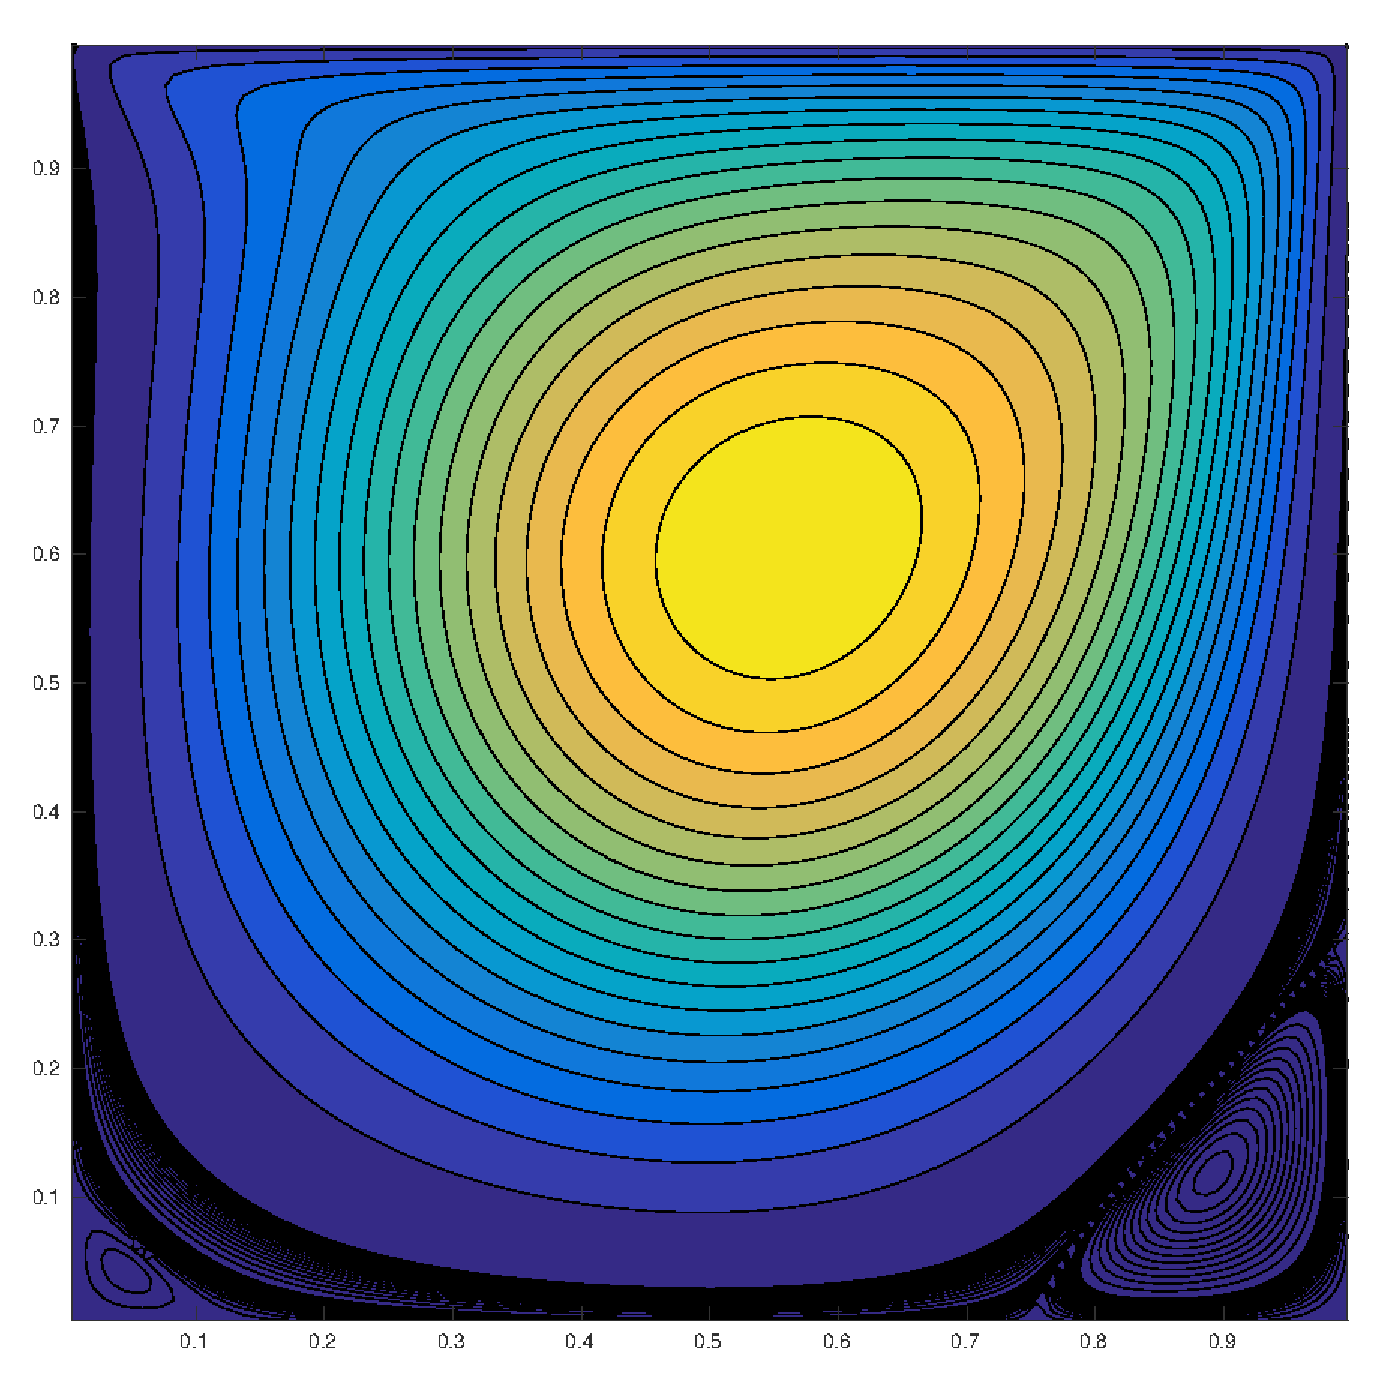
\includegraphics[width=0.4\textwidth]{Re400_streamf.eps}
      }	
 \subfloat[Vorticity contours at Re=100 ]{%
      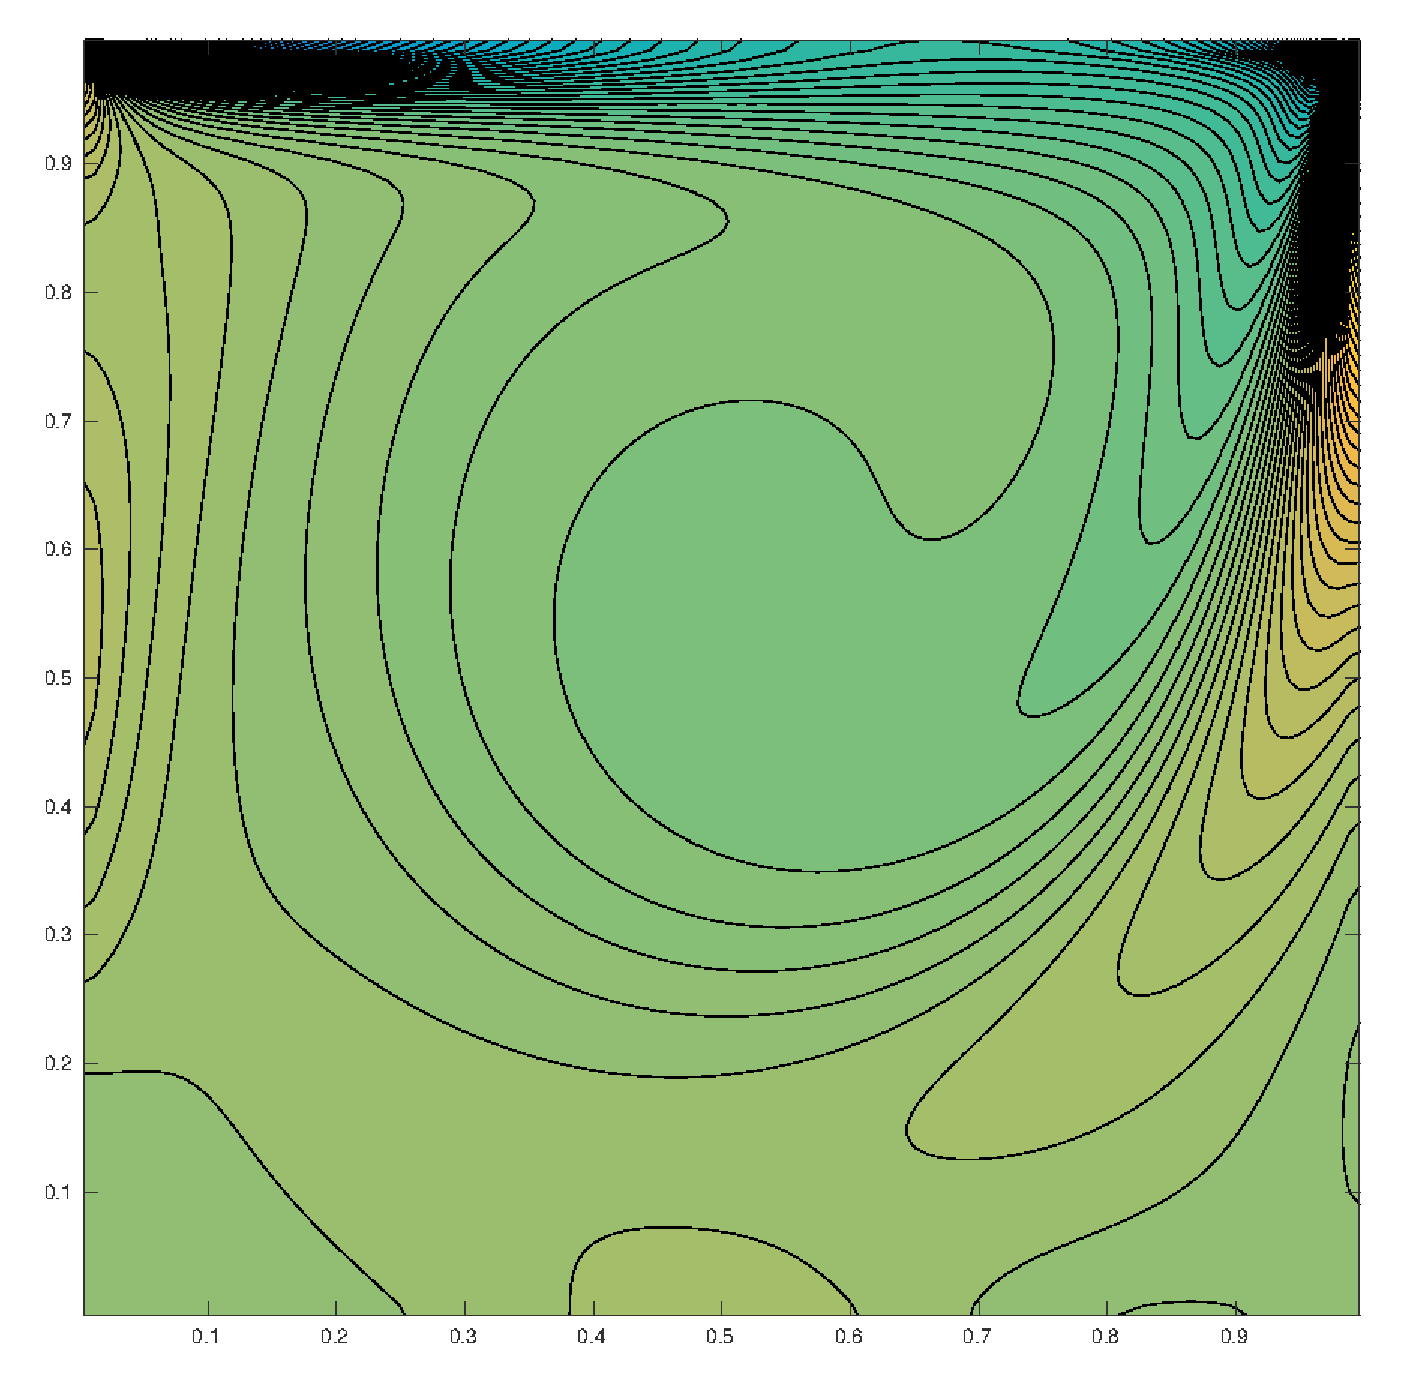
\includegraphics[width=0.4\textwidth]{Re400_vortf.eps}
      } \\
  \subfloat[Stream function contours at Re=1000 ]{%
      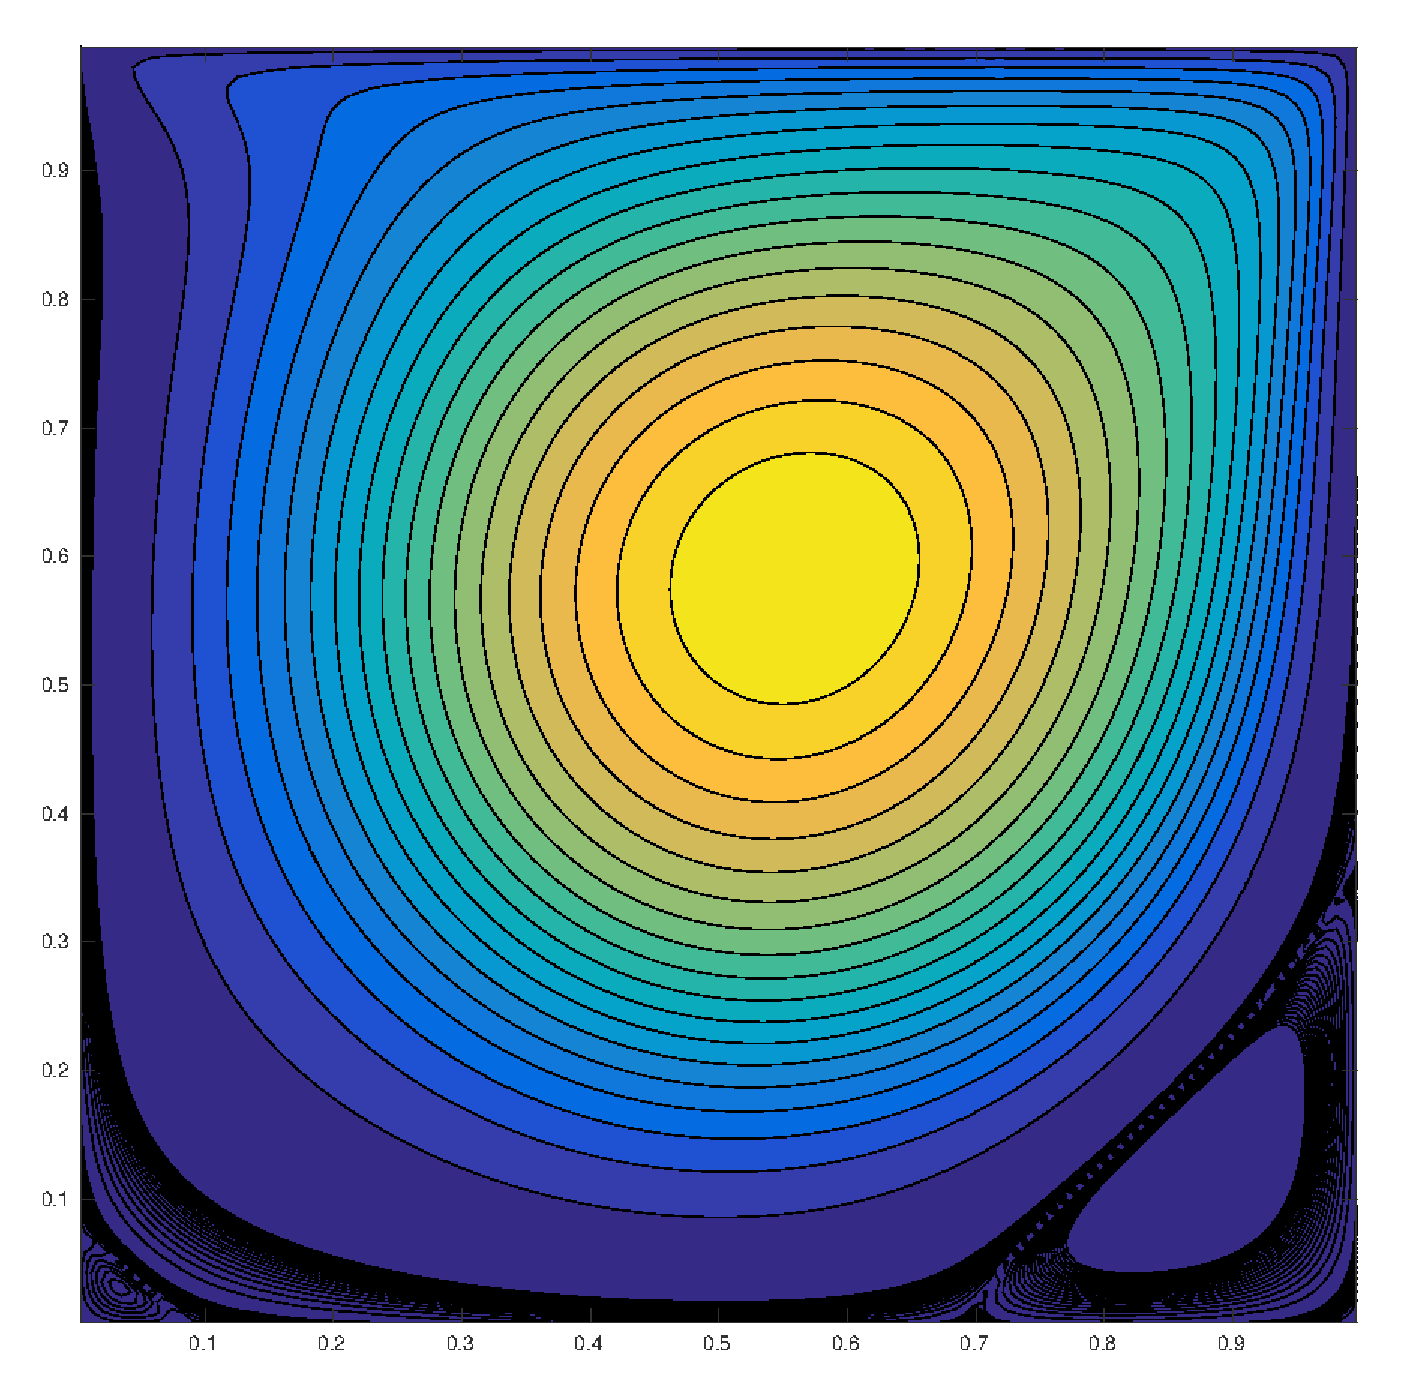
\includegraphics[width=0.4\textwidth]{Re1000_streamf.eps}
      }	
 \subfloat[Vorticity contours at Re=1000 ]{%
      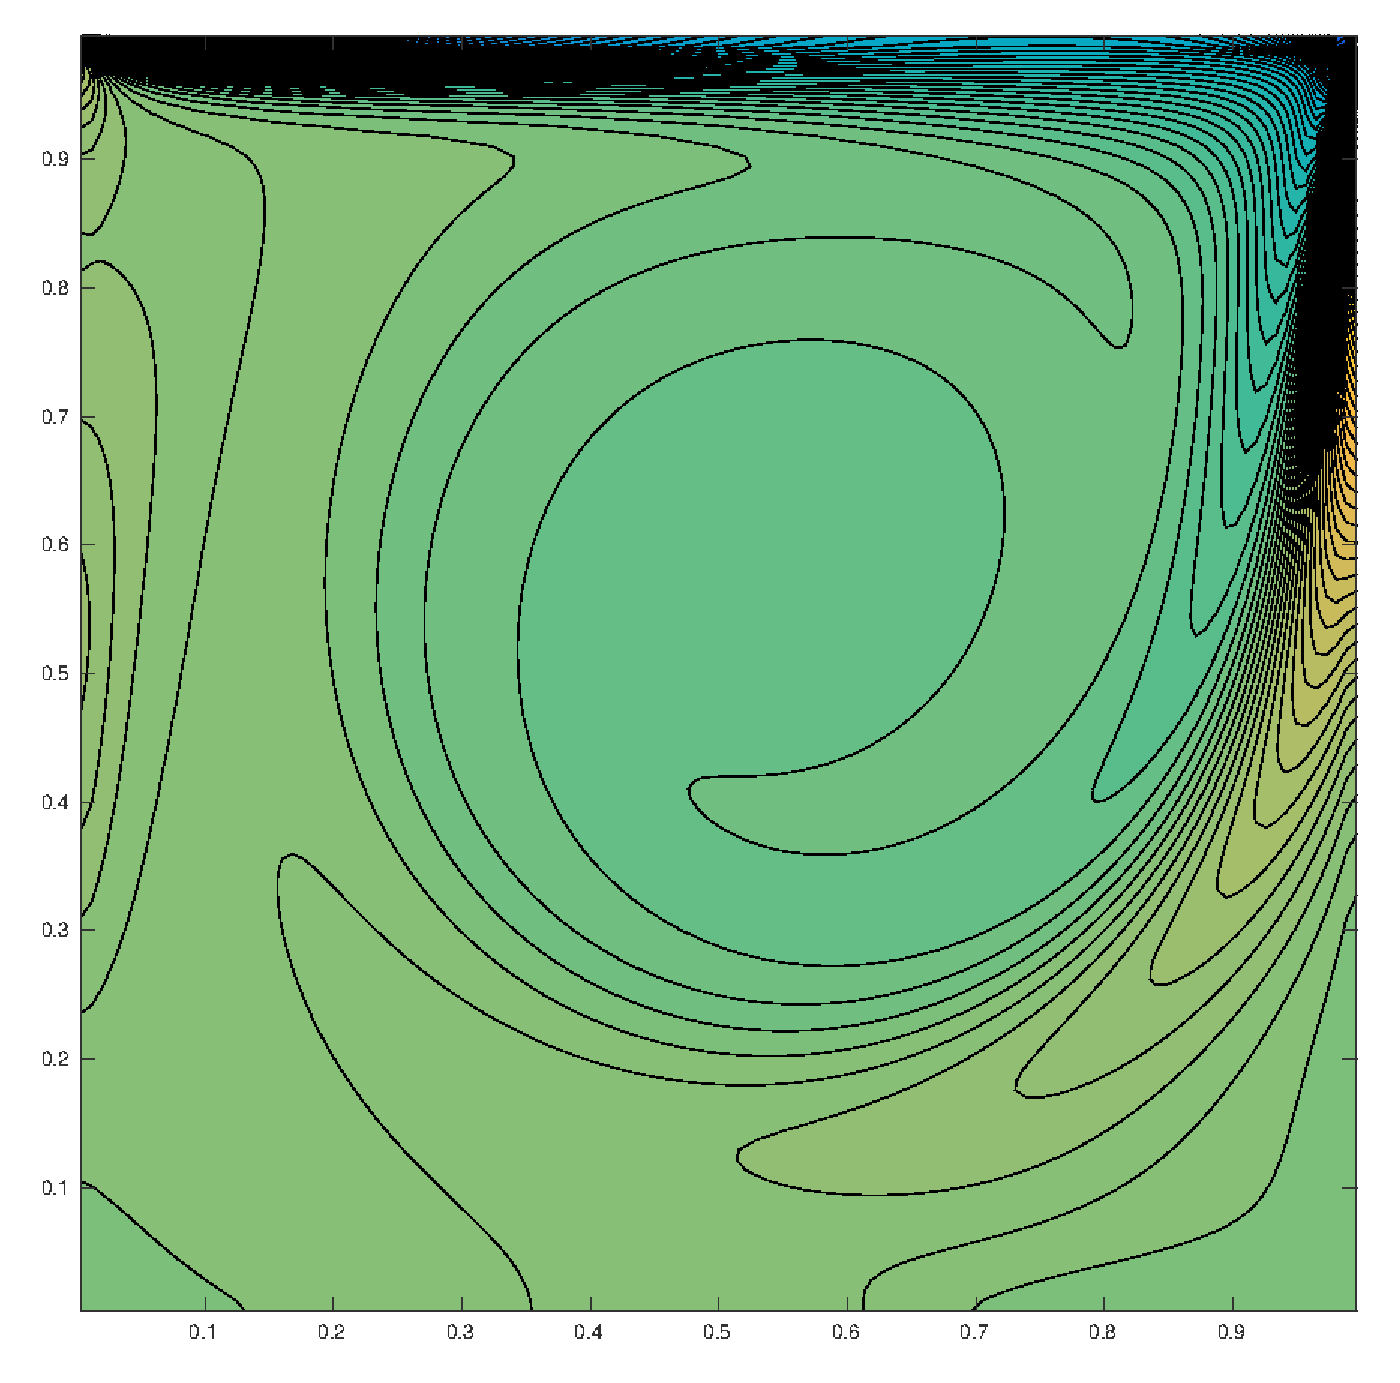
\includegraphics[width=0.4\textwidth]{Re1000_vortf.eps}
      }
 \caption{Stream function and vorticity contours}
 \label{Fig:cont1000}
\end{figure}

  \subsection{Falling Droplet}
 Falling droplet problem was set up and compared with Gerris simulations with exactly same input conditions (See Figure \ref{fd}).
 \begin{itemize}
 \item Domain: [0,3] x [0,3]
 \item Droplet: Diameter = 0.3, Center (1.5,2.5)
 \item Grid size: 96 x 96
 \item Time Step 0.00125
 \item Density ratio $\frac{\rho_G}{\rho_L}$, $\tilde\rho=0.5$
 \item Viscosity ratio $\frac{\mu_G}{\mu_L}$, $\tilde\mu=1.0$ 
 \item $Re_L=100$
 \item $Fr = 0.1$
  \item Boundary Condition : All walls no slip
 \end{itemize}
 
\begin{figure}
\subfloat[t = 0 ]{%
      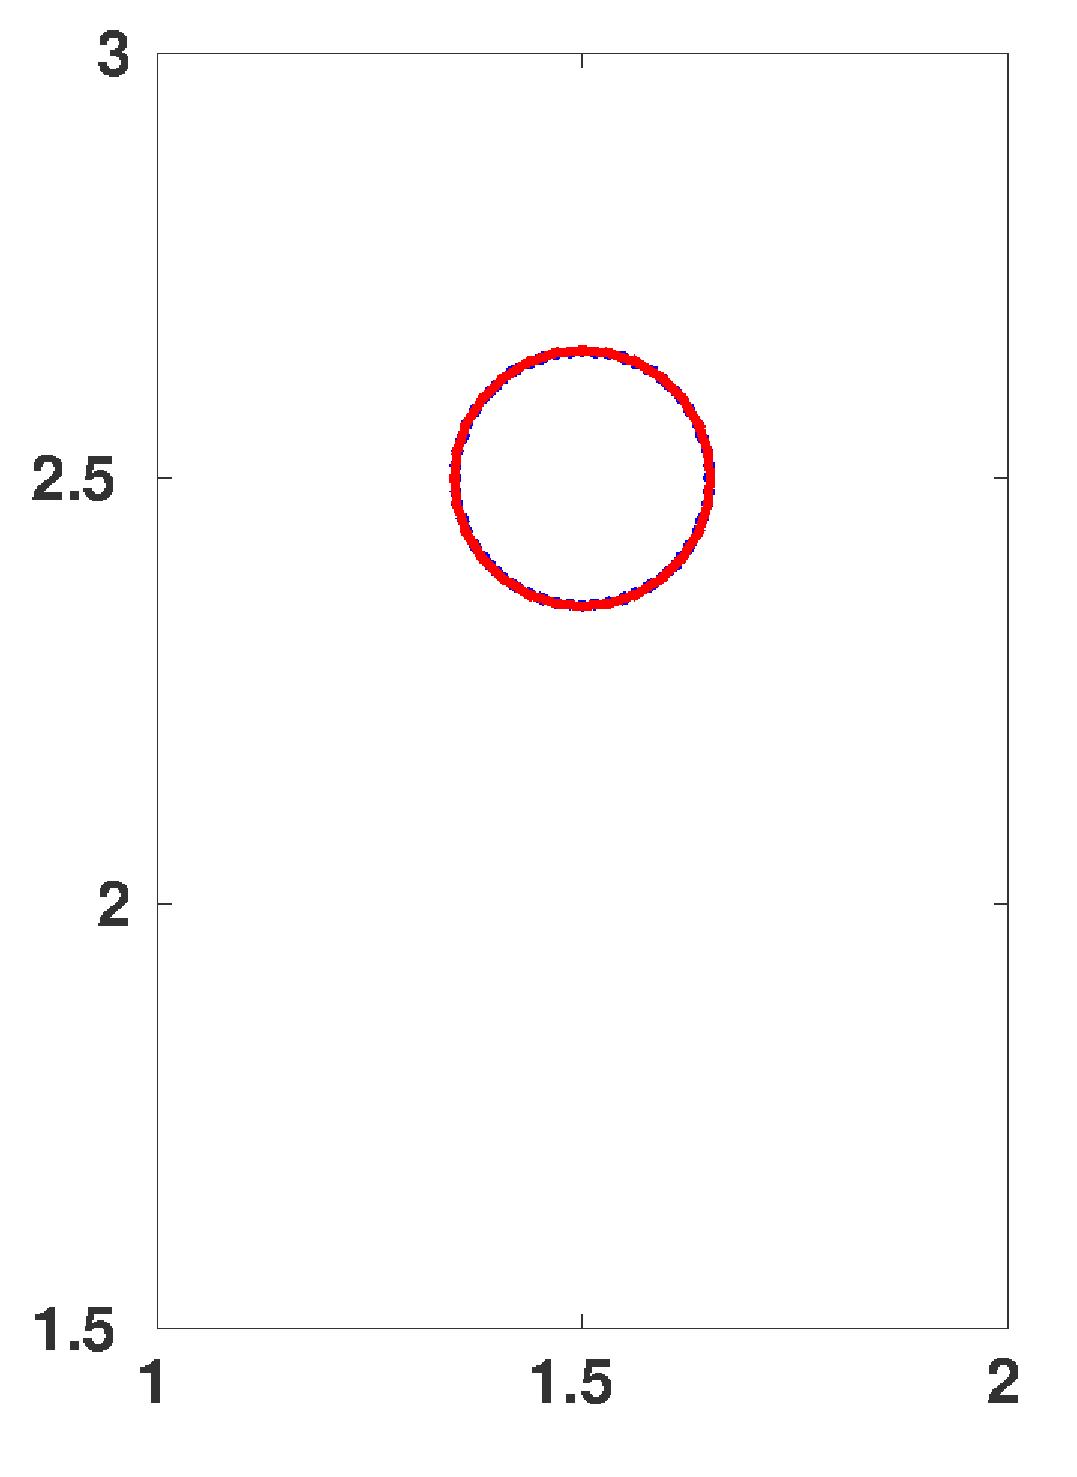
\includegraphics[width=0.5\textwidth]{drop_fall_0.eps}
      }
      \subfloat[t = 0.125 ]{%
      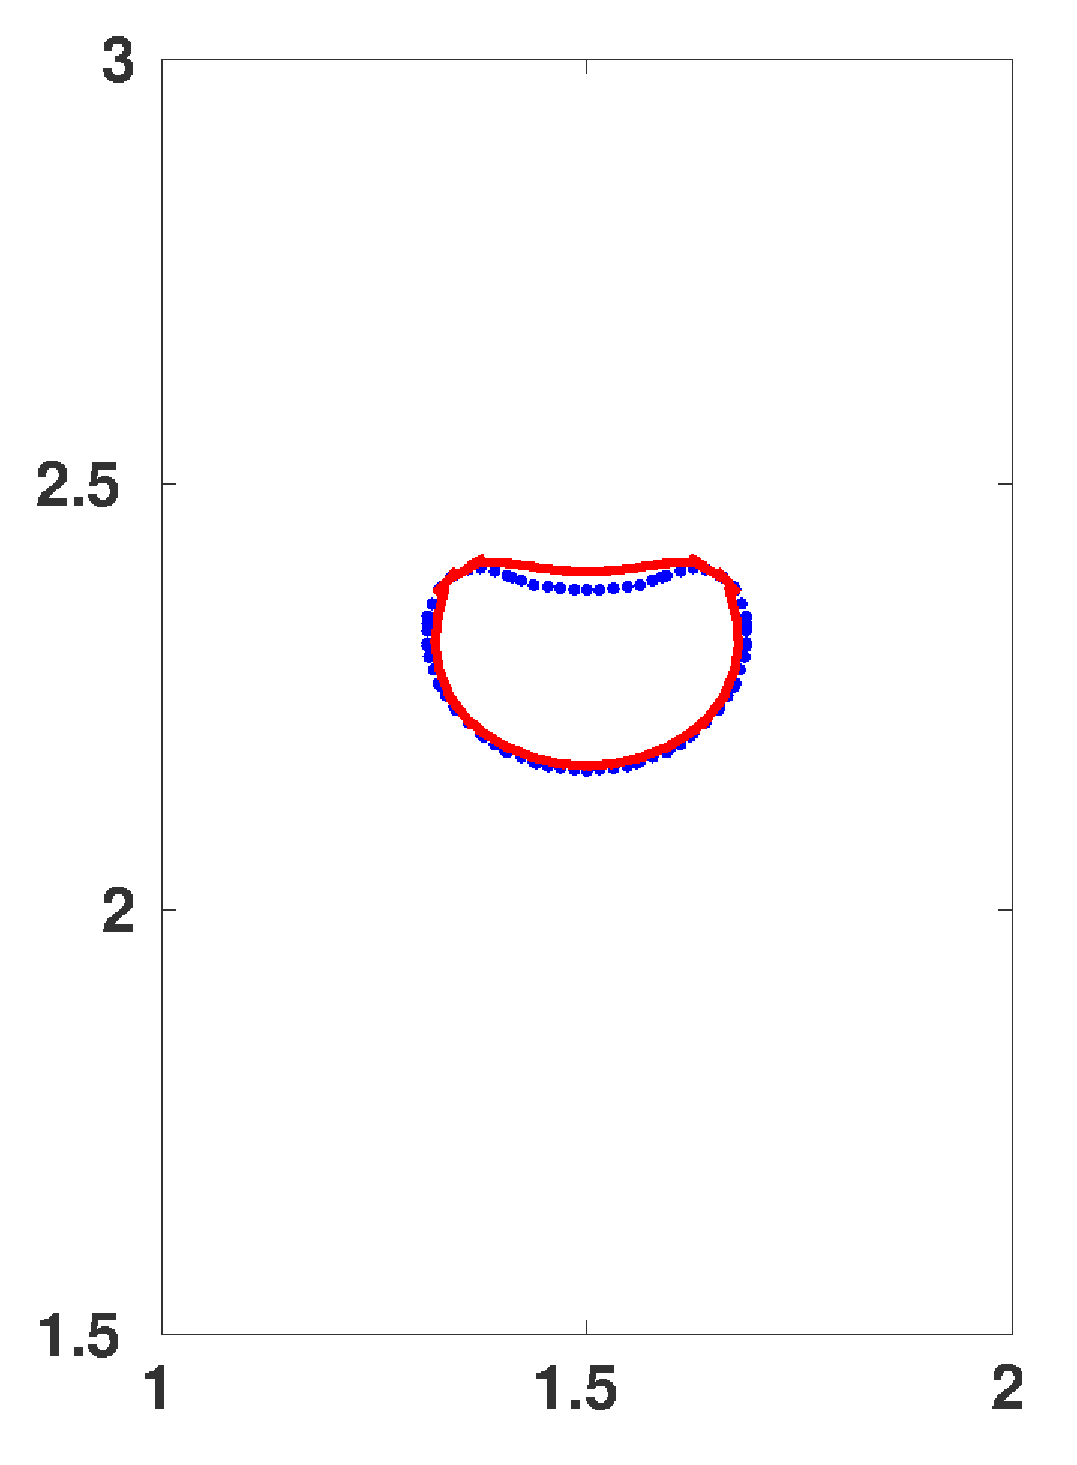
\includegraphics[width=0.5\textwidth]{drop_fall_100.eps}
      } \\
      \subfloat[t = 0.25 ]{%
      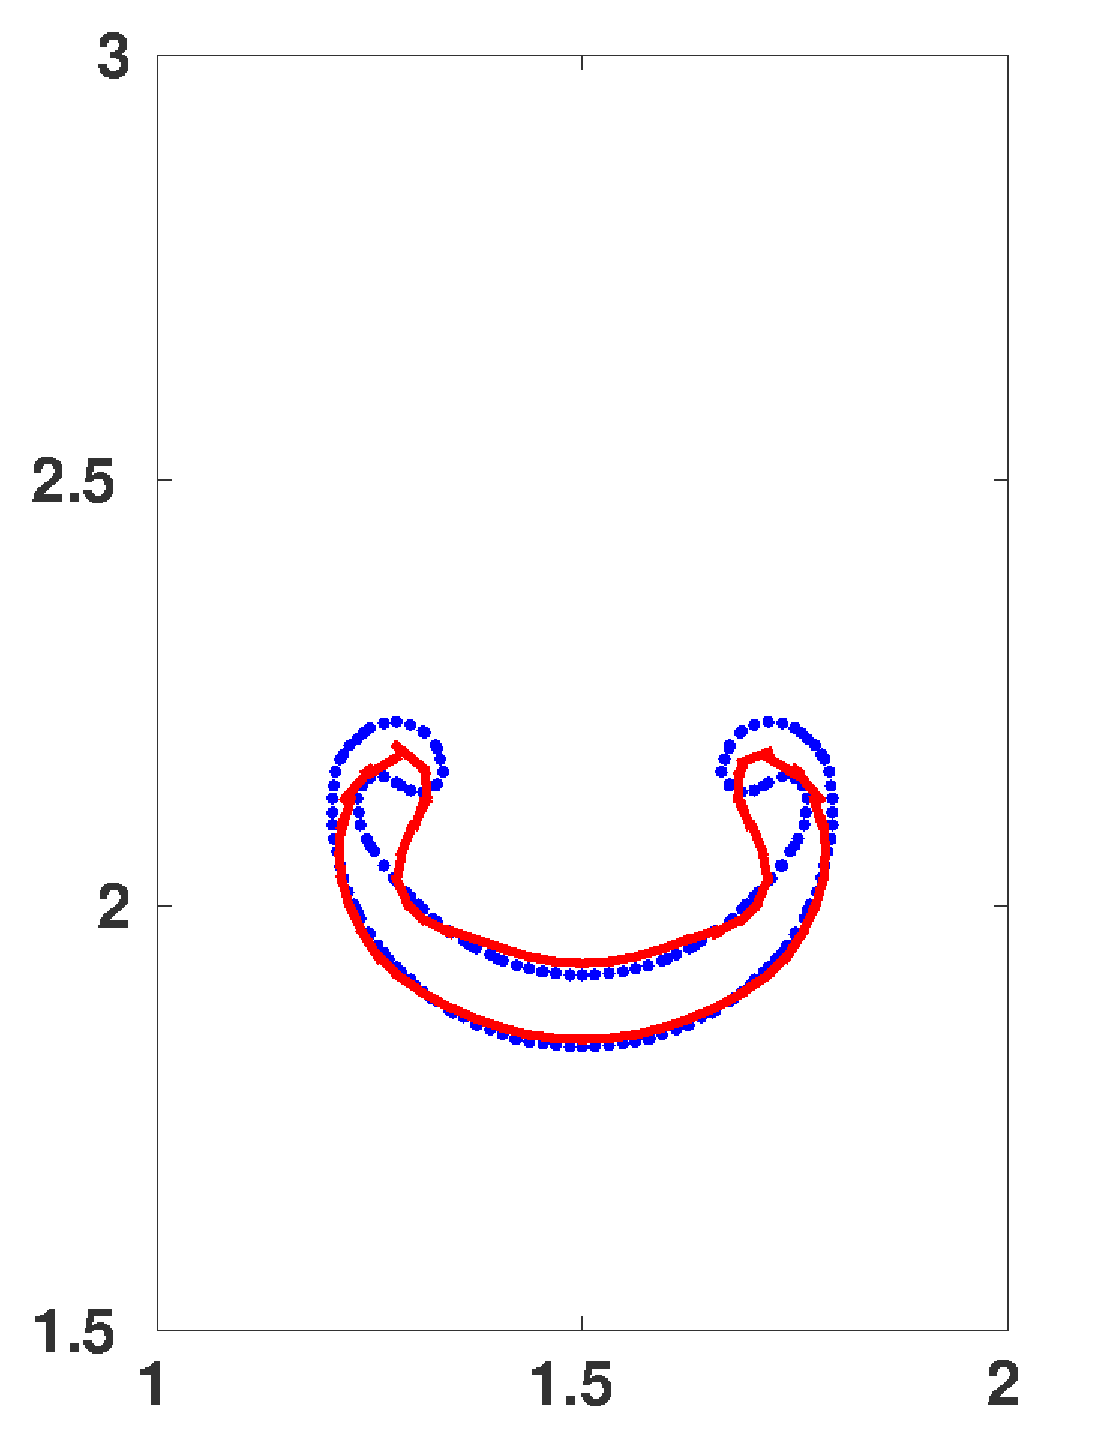
\includegraphics[width=0.5\textwidth]{drop_fall_200.eps}
      }
      \subfloat[t = 0.375 ]{%
      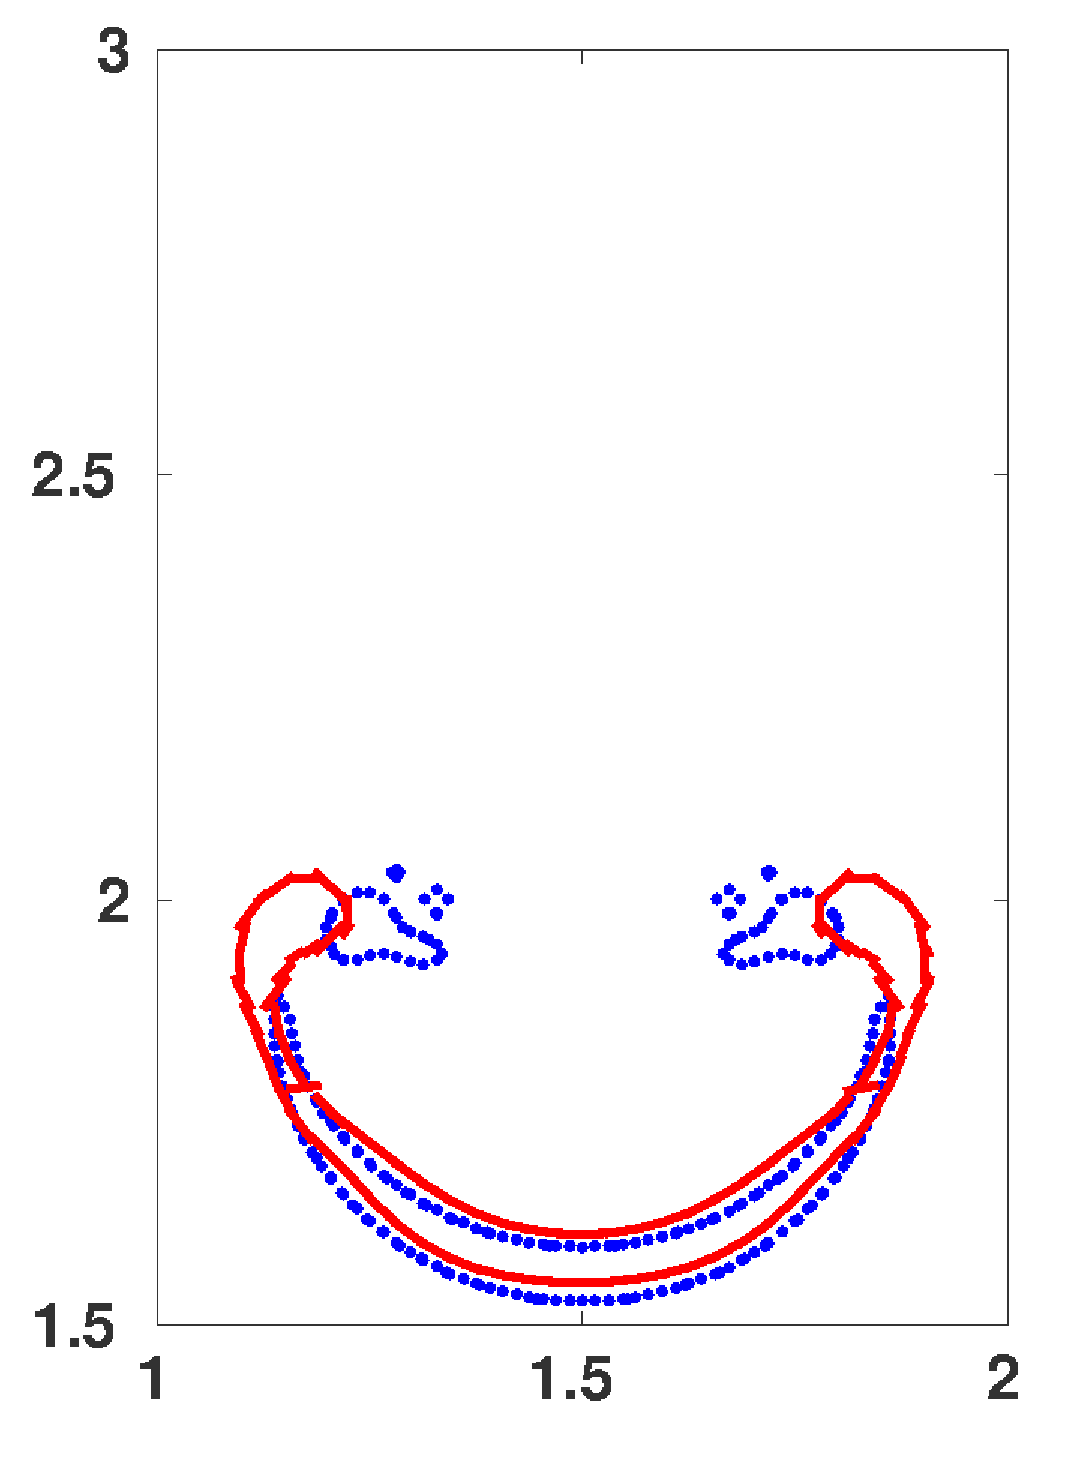
\includegraphics[width=0.5\textwidth]{drop_fall_300.eps}
      }
 \caption{Falling Droplet test, (Blue-Gerris, Red-Present Study(LVIRA))}
 \label{fd}
 \end{figure}
  
  \subsection{Rayleigh-Taylor Instability}
  Rayleigh-Taylor Instability is one of the most common test problems which are studied for verification, the problem was set up as in \cite{Rudman1997}
   \begin{enumerate}
 \item Domain: [0,1] x [0,3]
 \item Initial Interface: $y=2-0.02cos(\pi x)$
 \item Grid size: 64 x 192
 \item Time Step 0.005
 \item Density ratio $\frac{\rho_G}{\rho_L}$, $\tilde\rho=\frac{5}{6}$
 \item Viscosity ratio $\frac{\mu_G}{\mu_L}$, $\tilde\mu=1.0$ 
 \item $Re_L=500$
 \item $Fr = 0.5$
  \item Boundary Condition : top,bottom and right wall as no slip, left wall free slip
 \end{enumerate}
 Results are shown in Figure \ref{Fig:rudman}
 \begin{figure}
 \centering
 \subfloat[t = 0 ]{%
      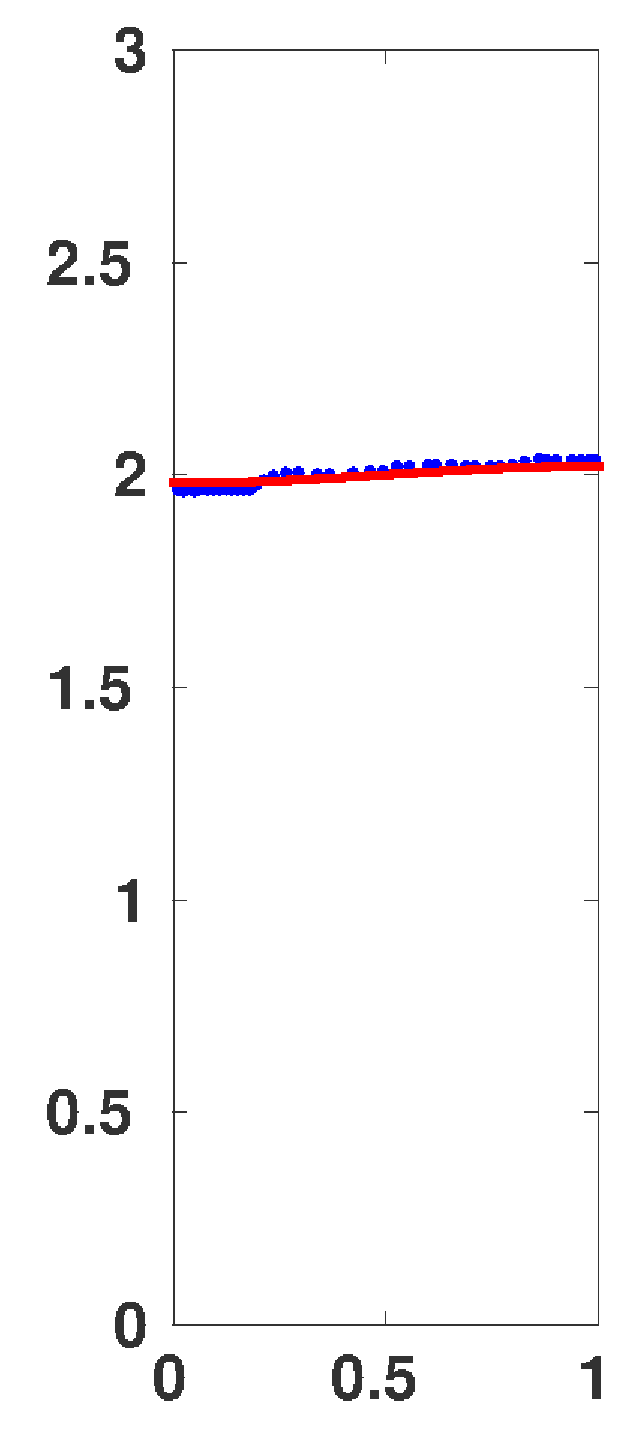
\includegraphics[width=0.3\textwidth]{Rudman_t0.eps}
      }
  \subfloat[t = 4 ]{%
      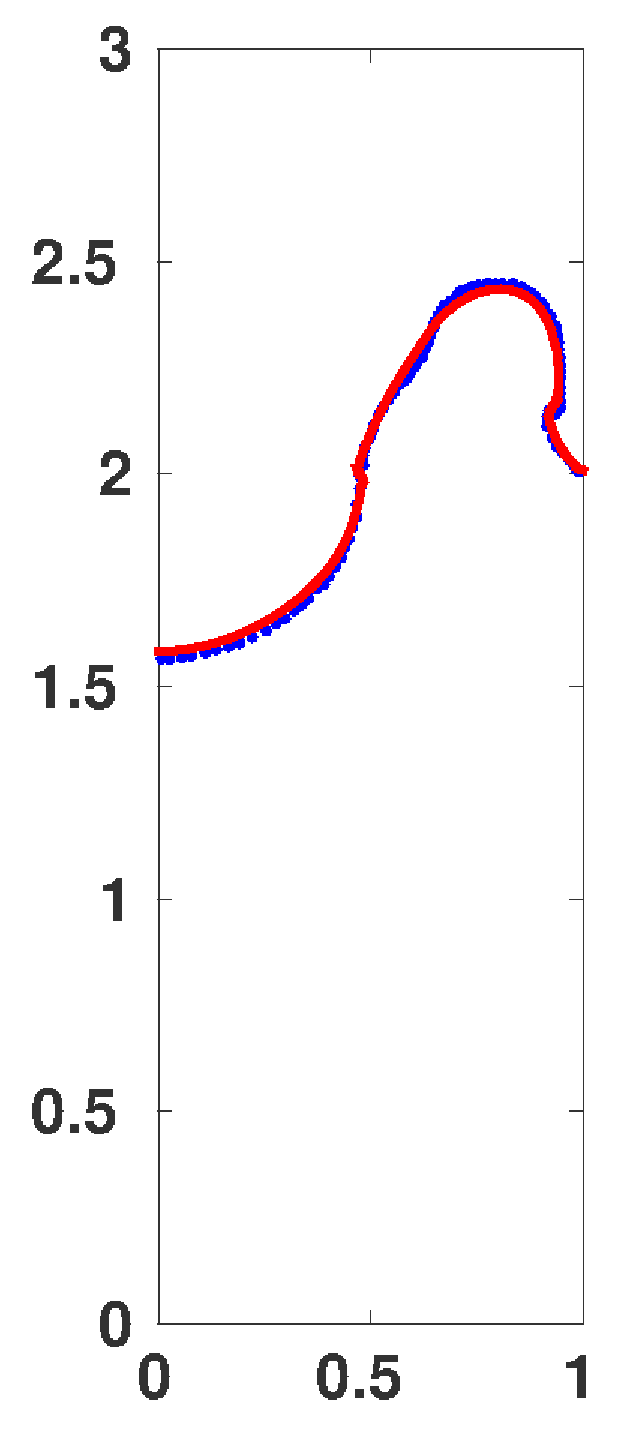
\includegraphics[width=0.3\textwidth]{Rudman_t4.eps}
      } \\
       \subfloat[t = 6 ]{%
      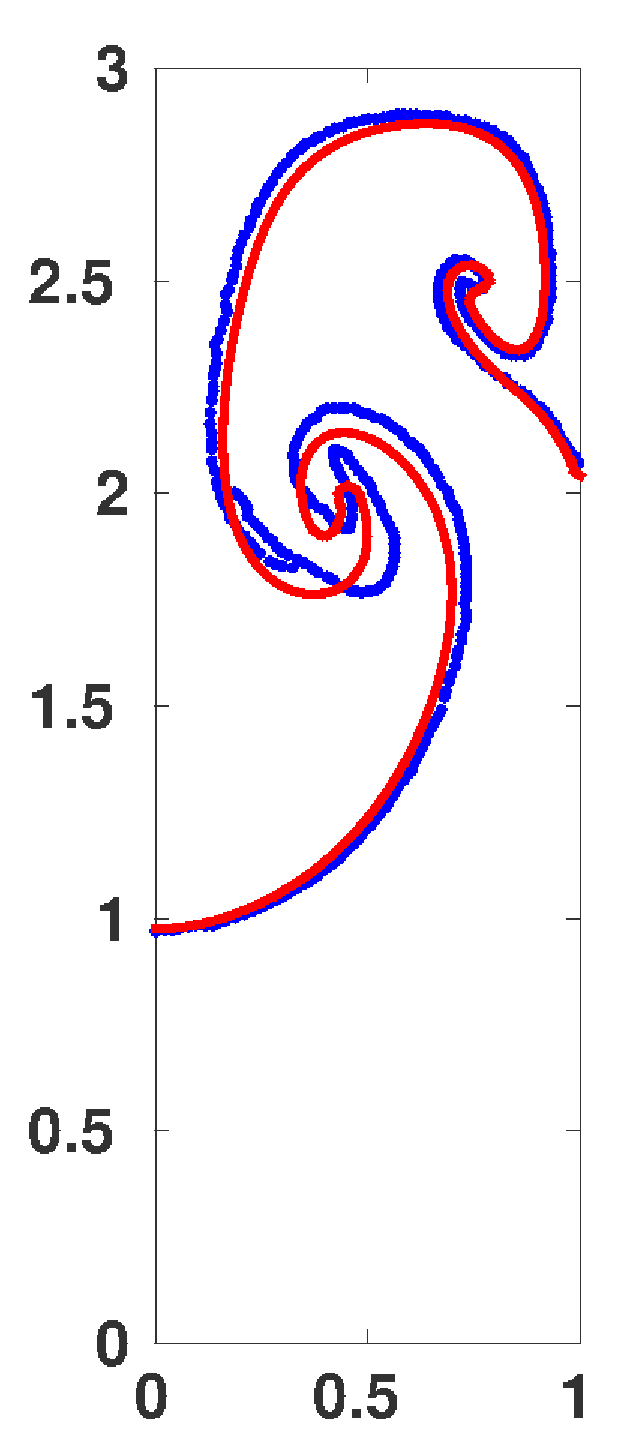
\includegraphics[width=0.3\textwidth]{Rudman_t6.eps}
      }
       \subfloat[t = 8 ]{%
      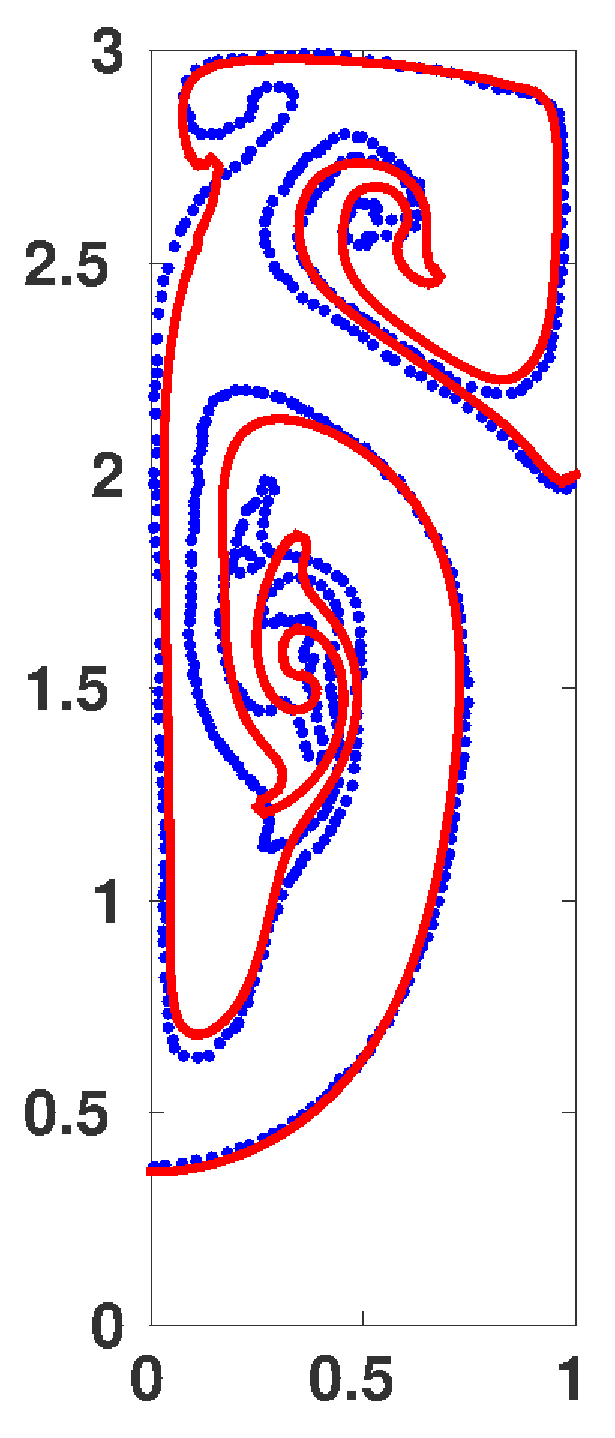
\includegraphics[width=0.3\textwidth]{Rudman_t8.eps}
      }
 \caption{Comparison of Rayleigh-Taylor Instability test,(Blue-\cite{Rudman1997}, Red-Present Study(LVIRA))}
  \label{Fig:rudman}
 \end{figure}
 
 Similar problem with different initial and boundary conditions was studies and compared with \cite{Anton2001} as shown in Figure \ref{Fig:anton}
    \begin{enumerate}
 \item Domain: [0,1] x [0,4]
 \item Initial Interface: $y=2+0.05cos(2\pi x)$
 \item Grid size: 40 x 160
 \item Time Step 0.001
 \item Density ratio $\frac{\rho_G}{\rho_L}$, $\tilde\rho=\frac{17}{120}$
 \item Viscosity ratio $\frac{\mu_G}{\mu_L}$, $\tilde\mu=1.0$ 
 \item $Re_L=\frac{1000}{3}$
 \item $Fr = 1.0$
 \item Boundary Condition : top and bottom wall as no slip, left and right wall free slip
 \end{enumerate}
 
  \begin{figure}
 \centering
 \subfloat[t = 0 ]{%
      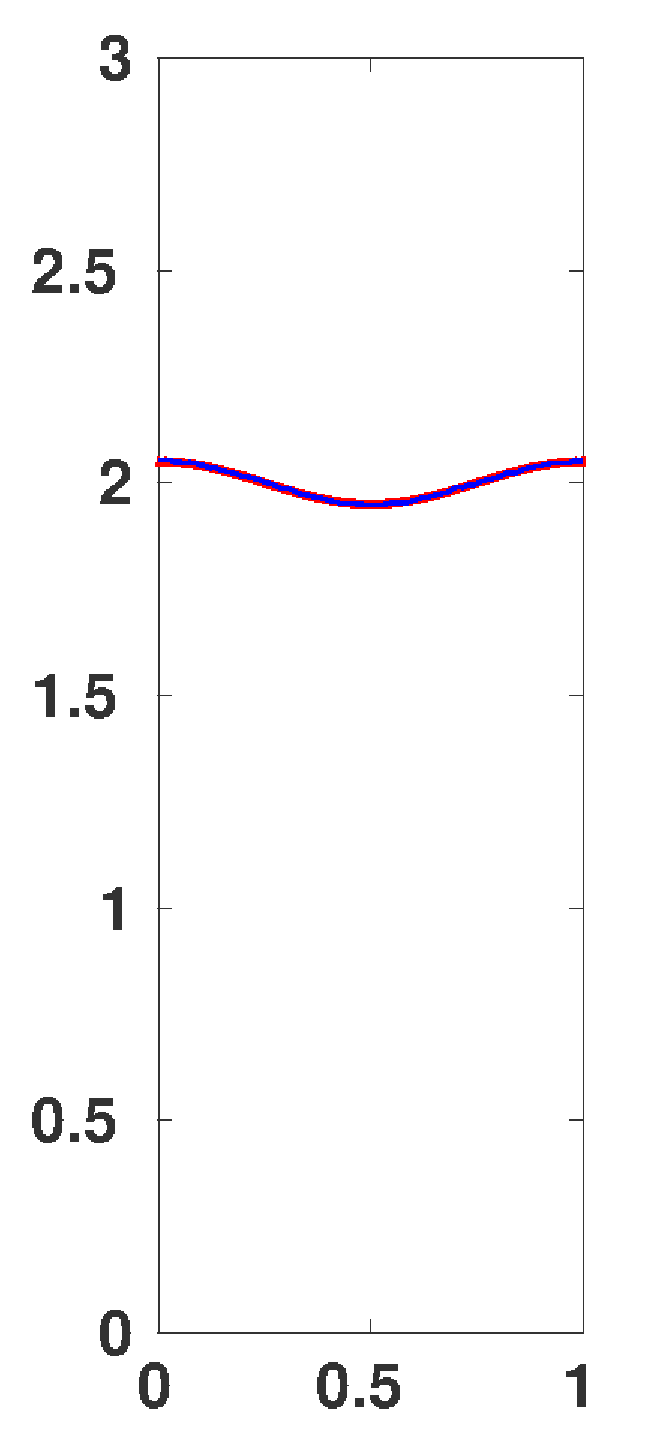
\includegraphics[width=0.3\textwidth]{anton-t0.0.eps}
      }
  \subfloat[t = 1.9 ]{%
      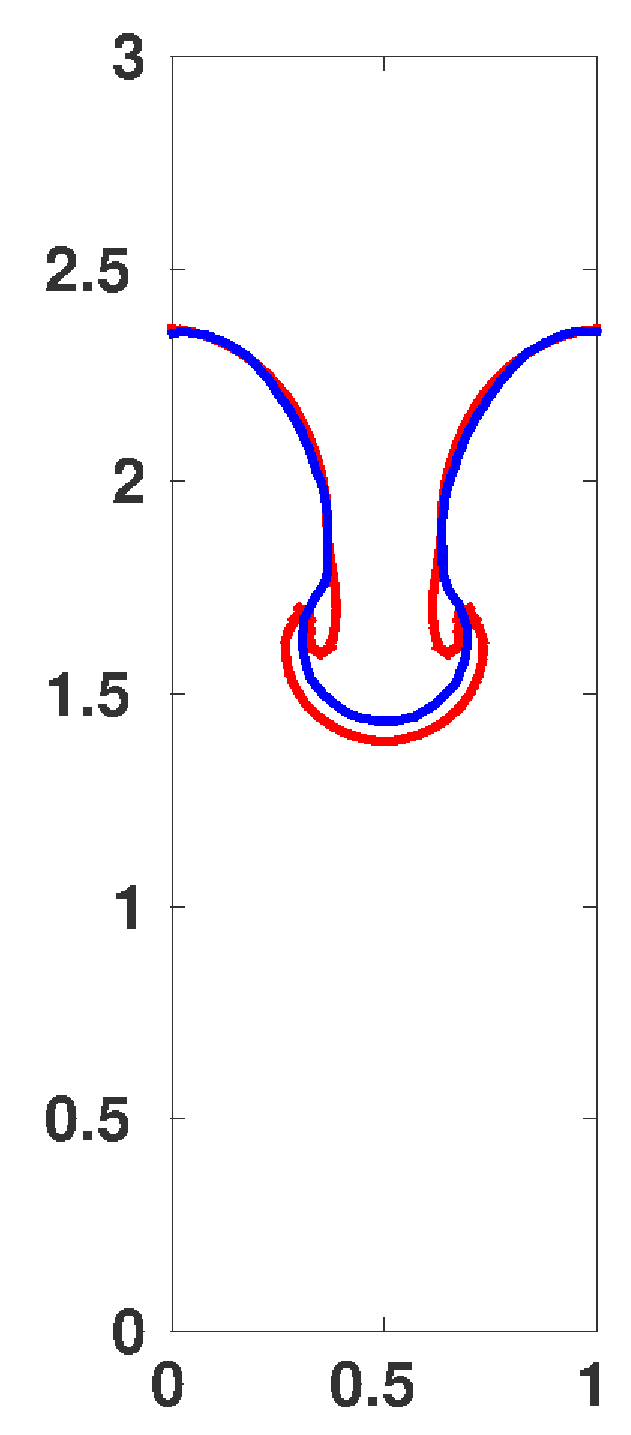
\includegraphics[width=0.3\textwidth]{anton-t1.9.eps}
      } \\
       \subfloat[t = 2.6 ]{%
      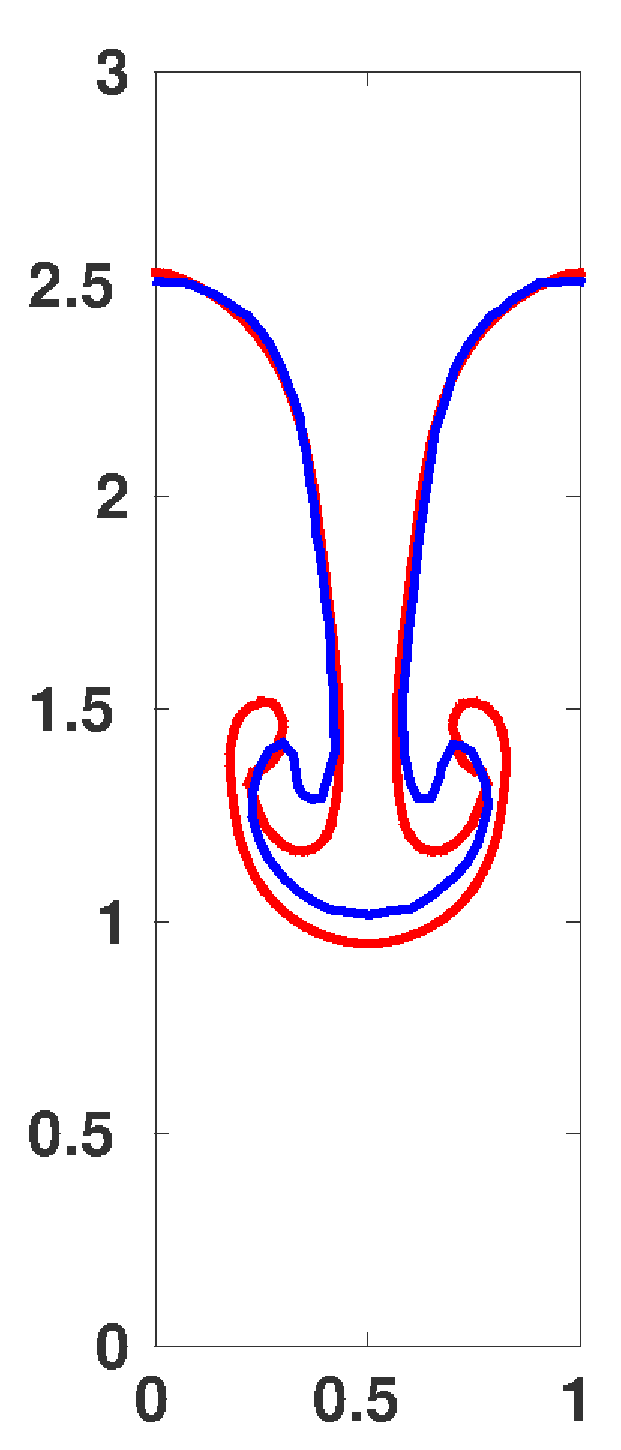
\includegraphics[width=0.3\textwidth]{anton-t2.6.eps}
      }
       \subfloat[t = 3.3 ]{%
      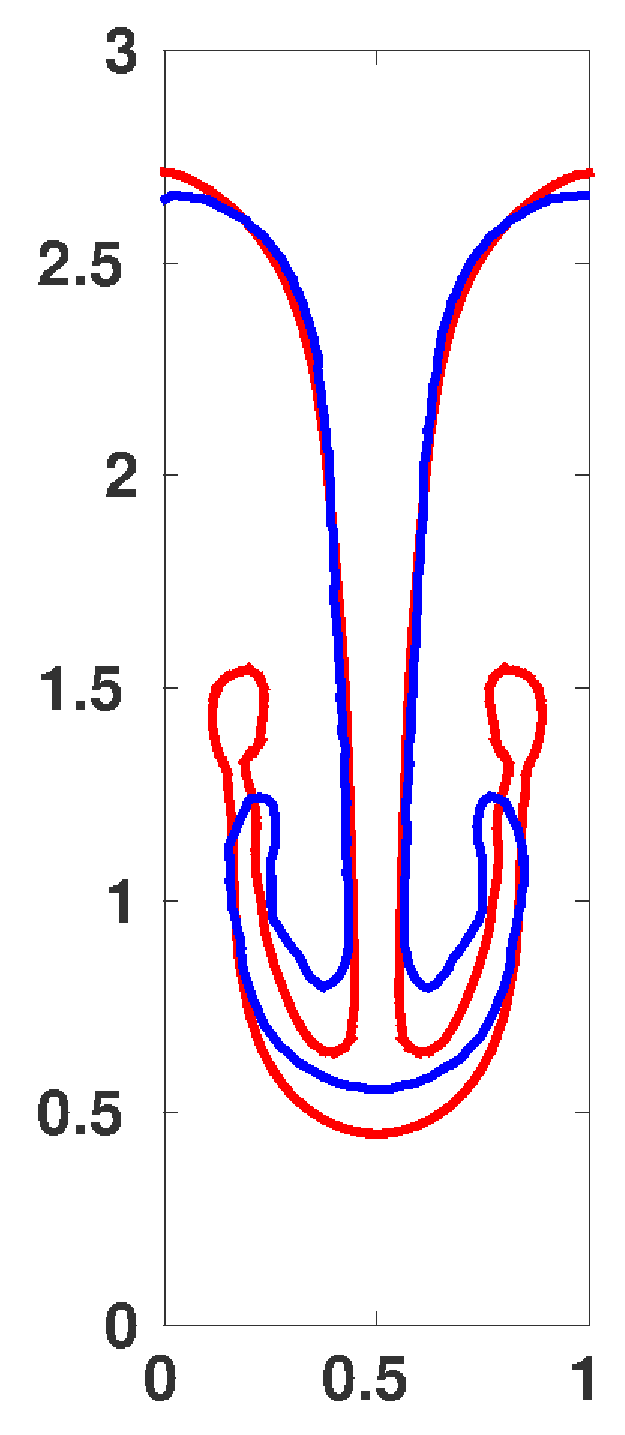
\includegraphics[width=0.3\textwidth]{anton-t3.3.eps}
      }
    \subfloat[t = 4.0 ]{%
      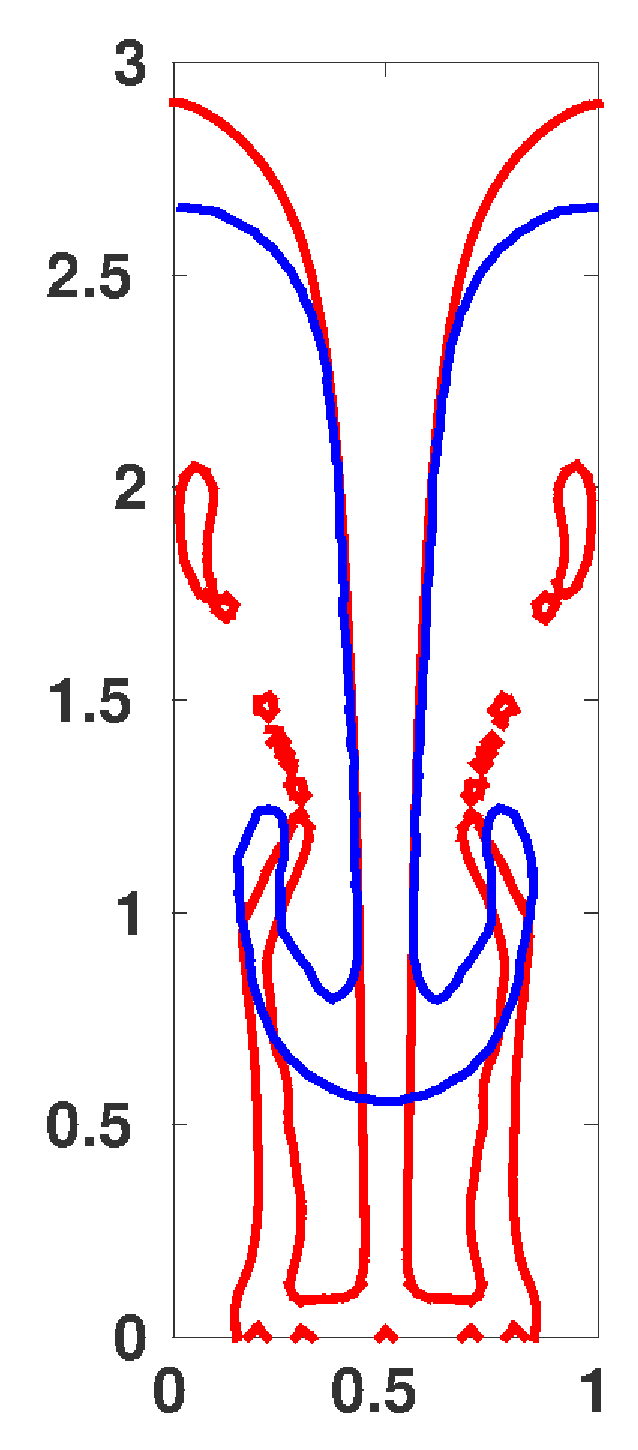
\includegraphics[width=0.3\textwidth]{anton-t4.0.eps}
      }
 \caption{Comparison of Rayleigh-Taylor Instability test,(Blue-\cite{Anton2001}, Red-Present Study(LVIRA))}
 \label{Fig:anton}
 \end{figure}
 
\section{Conclusion} 
 The solver however produce satisfactory results while benchmarking but there is a need to improve the accuracy,
 for which we plan to implement advance advection schemes such as Godunov scheme.
 Also, Gauss-Sidel method used to solve pressure poisson equation converges very slowly
 and results in extensive use of computational resources and time. 
 To improve the effciency, we plan to use multigrid methods to solve the pressure poisson equation.
 
 
 
 
 
 